\documentclass[semifinal]{cpecmu}

%% This is a sample document demonstrating how to use the CPECMU
%% project template. If you are having trouble, see "cpecmu.pdf" for
%% documentation.

\projectNo{P011-2/68}
\acadyear{2025}

\titleTH{ระบบบริหารจัดการพลังงานอัจฉริยะเพื่อมุ่งสู่ความเป็นกลางทางคาร์บอนในอาคาร}
\titleEN{Smart Energy Management System for Carbon Neutrality in Buildings}

\author{นางสาวธณิชา มังกร}{Mrs. Thanicha Mangkorn}{650610764}
\author{นายปุณณวิชญ์ เดชอินทร์}{Mr. Punnawich Dach-in}{650610787}
\author{นายรัชพล แปรงทอง}{Mr. Ratchapon Prangthong}{650610802}

\cpeadvisor{paskorn}
\cpecommittee{pruet}
\cpecommittee{yuthapong}
% \committee{รศ.ดร.\,นิพนธ์ ธีรอำพน}{Assoc.\,Prof.\,Nipon Theera-Umpon, Ph.D.}

%% Some possible packages to include:
\usepackage[final]{graphicx} % for including graphics

%% Add bookmarks and hyperlinks in the document.
\PassOptionsToPackage{hyphens}{url}
\usepackage[colorlinks=true,allcolors=Blue4,citecolor=red,linktoc=all]{hyperref}
\def\UrlLeft#1\UrlRight{$#1$}

%% Needed just by this example, but maybe not by most reports
\usepackage{afterpage} % for outputting
\usepackage{pdflscape} % for landscape figures and tables. 

%% Some other useful packages. Look these up to find out how to use
%% them.
% \usepackage{natbib}    % for author-year citation styles
% \usepackage{txfonts}
% \usepackage{appendix}  % for appendices on a per-chapter basis
% \usepackage{xtab}      % for tables that go over multiple pages
% \usepackage{subfigure} % for subfigures within a figure
% \usepackage{pstricks,pdftricks} % for access to special PostScript and PDF commands
% \usepackage{nomencl}   % if you have a list of abbreviations

%% if you're having problems with overfull boxes, you may need to increase
%% the tolerance to 9999
% \tolerance=9999

\bibliographystyle{plain}
% \bibliographystyle{IEEEbib}

% \renewcommand{\topfraction}{0.85}
% \renewcommand{\textfraction}{0.1}
% \renewcommand{\floatpagefraction}{0.75}

%% Example for glossary entry
%% Need to use glossary option
%% See glossaries package for complete documentation.
\ifglossary
  \newglossaryentry{lorem ipsum}{
    name=lorem ipsum,
    description={derived from Latin dolorem ipsum, translated as ``pain itself''}
  }
\fi

%% Uncomment this command to preview only specified LaTeX file(s)
%% imported with \include command below.
%% Any other file imported via \include but not specified here will not
%% be previewed.
%% Useful if your report is large, as you might not want to build
%% the entire file when editing a certain part of your report.
% \includeonly{chapters/intro,chapters/background}
\usepackage{caption}
\captionsetup{
    justification=centering, % จัดข้อความทุกบรรทัดให้อยู่กึ่งกลาง
    singlelinecheck=false,   % บังคับกึ่งกลางแม้จะมีข้อความเพียงบรรทัดเดียว
    font=small,              % (ตัวเลือกเสริม) ปรับขนาดตัวอักษรให้เล็กกว่าเนื้อหาเล็กน้อย
    labelfont=bf             % (ตัวเลือกเสริม) ทำตัวหนาที่คำว่า "รูปที่ X.Y"
}
\usepackage{float}
\usepackage{multirow}
\usepackage{graphicx}

\begin{document}
\maketitle
\makesignature

\ifproject
\begin{abstractTH}
\sloppy

% เขียนบทคัดย่อของโครงงานที่นี่
\hspace{\parindent}ปัจจุบันมหาวิทยาลัยเชียงใหม่มีการติดตั้งระบบโซลาร์เซลล์แล้วแต่ยังพบความไม่สอดคล้องระหว่างการใช้ไฟฟ้าและปริมาณการผลิตไฟฟ้าจากเซลล์แสงอาทิตย์ (Solar Cell) 
เนื่องจากพลังงานที่ผลิตได้ขึ้นอยู่กับสภาพอากาศมีการเปลี่ยนแปลงตลอดเวลา
อย่างไรก็ตาม ระบบในปัจจุบันยังไม่มีข้อมูลสภาพอากาศที่ละเอียดเพียงพอสำหรับการวิเคราะห์หรือคาดการณ์การผลิตพลังงาน ส่งผลให้ไม่สามารถวางแผนการใช้พลังงานได้อย่างมีประสิทธิภาพ

เพื่อแก้ไขปัญหานี้ โครงการจึงพัฒนาสถานีตรวจวัดสภาพอากาศขนาดย่อมสำหรับเก็บข้อมูลสิ่งแวดล้อมที่มีผลต่อการผลิตไฟฟ้าจากเซลล์แสงอาทิตย์ (Solar Cell) โดยใช้เซ็นเซอร์วัดอุณหภูมิ ความชื้นสัมพัทธ์ ความกดอากาศ ความเข้มของแสง อุณภูมิแผงโซลาร์เซลล์ ความเร็วลม และทิศทางลม 
ข้อมูลที่ได้จะถูกนำไปใช้ในการวิเคราะห์และสร้างแบบจำลองเพื่อทำนายการผลิตพลังงานจากเซลล์แสงอาทิตย์ (Solar Cell) ล่วงหน้า 24 ชั่วโมง ซึ่งจะช่วยให้สามารถวางแผนการใช้งานพลังงานและบริหารจัดการพลังงานได้อย่างมีประสิทธิภาพมากขึ้นซึ่งไม่เพียงแต่ช่วยลดค่าใช้จ่ายด้านพลังงาน แต่ยังเป็นการสนับสนุนนโยบายการลดการปล่อยก๊าซเรือนกระจกและมุ่งสู่ความเป็นกลางทางคาร์บอนในอาคารของมหาวิทยาลัย
\end{abstractTH}

\begin{abstract}
    \hspace{\parindent}Currently, Chiang Mai University has implemented solar cell systems to promote renewable energy. However, there is still a discrepancy between electricity consumption and the actual power generated from solar energy, primarily due to the intermittent nature of solar power which fluctuates according to weather conditions. Furthermore, existing systems lack high-resolution meteorological data necessary for accurate analysis or forecasting, leading to challenges in efficient energy planning.
 
    To address this issue, the project developed a compact weather station to collect environmental data affecting solar power generation, including temperature, relative humidity, air pressure, solar intensity, solar panel temperature, wind speed, and wind direction. The gathered data is utilized for analysis and modeling to predict solar energy output 24 hours in advance. This enables more efficient energy planning and management, which not only reduces energy costs but also supports greenhouse gas reduction policies and the university's goal of achieving carbon neutrality.
\end{abstract}

\iffalse
\begin{dedication}
This document is dedicated to all Chiang Mai University students.

Dedication page is optional.
\end{dedication}
\fi % \iffalse

\begin{acknowledgments}
\sloppy
\hspace{\parindent}โครงการ ระบบบริหารการจัดการพลังงานอัจฉริยะเพื่อมุ่งสู่ความเป็นกลางทางคาร์บอนภายในอาคาร (Smart Energy Management System for Carbon Neutrality in Buildings) ไม่อาจสําเร็จลุล่วงได้ หากปราศจากแรงสนับสนุน คําแนะนํา และความทุ่มเทจาก
หลายฝ่ายทั้ง ผศ.ดร.ภาสกร แช่มประเสริฐ อาจารย์ที่ปรึกษาที่ได้สละเวลาอันมีค่าในการให้คำปรึกษา แนะนำแนวคิด ตลอดจนถ่ายทอดความรู้และประสบการณ์ที่เป็นประโยชน์ยิ่ง ทำให้คณะผู้จัดทำสามารถแก้ไขปัญหาและดำเนินงานได้อย่างมีประสิทธิภาพ

ขอขอบพระคุณ ผศ.ดร.พฤษภ์ บุญมา และ ผศ.ดร.ยุทธพงษ์ สมจิต 
อาจารย์กรรมการสอบโครงการ ที่สละเวลาในวันเวลาสอบเพื่อตรวจสอบ ให้ข้อเสนอแนะ และแนะนําแนวทางในการ
ปรับปรุงระบบให้มีคุณภาพและความสมบูรณ์ยิ่งขึ้น

นอกจากนี้ คณะผู้จัดทำขอขอบคุณรุ่นพี่และเพื่อนที่คอยช่วยทดสอบระบบ และคอยให้คําแนะนําต่างๆ
คณะผู้จัดทำขอถือโอกาสนี้แสดงความขอบคุณจากใจจริงต่อทุกภาคส่วนที่มีส่วนร่วมในการผลักดันให้โครงการนี้เกิดขึ้น

\acksign{2026}{3}{20}
\end{acknowledgments}%
\fi % \ifproject

\contentspage

\ifproject
\figurelistpage

\tablelistpage
\fi % \ifproject

% \abbrlist % this page is optional

% \symlist % this page is optional

% \preface % this section is optional


\pagestyle{empty}\cleardoublepage
\normalspacing \setcounter{page}{1} \pagenumbering{arabic} \pagestyle{cpecmu}

\chapter{\ifenglish Introduction\else บทนำ\fi}

\section{\ifenglish Project rationale\else ที่มาของโครงงาน\fi}
ในปัจจุบันองค์กรและสถาบันการศึกษาต่างๆ รวมถึงมหาวิทยาลัยเชียงใหม่มีการใช้พลังงานไฟฟ้า 
เพิ่มขึ้นอย่างต่อเนื่อง ส่งผลให้เกิดการปล่อยก๊าซคาร์บอนไดออกไซด์ในปริมาณมาก ถึงแม้ว่า 
มหาวิทยาลัยเชียงใหม่จะมีการติดตั้งระบบผลิตไฟฟ้าจากเซลล์แสงอาทิตย์ (Solar Cell) แล้วก็ตาม 
เนื่องจากทางมหาวิทยาลัยเชียงใหมยังไม่มีระบบจัดเก็บพลังงานสำรอง (Battery) 
ทำให้การผลิตไฟฟ้าไม่สอดคล้องกับการใช้งานจริงส่งผลให้มหาวิทยาลัยเชียงใหม่ต้องพึ่งพาพลังงานไฟฟ้าจาก
ภายนอก (PEA) มากกว่าการใช้พลังงานไฟฟ้าที่ผลิตได้ นอกจากนี้ การผลิตไฟฟ้าจากพลังงานแสงอาทิตย์ 
(Solar Cell) ยังมีความไม่แน่นอน เนื่องจากขึ้นอยู่กับสภาพอากาศที่เปลี่ยนแปลงลงตลอดเวลา
ทำให้การวางแผนการใช้พลังงานไฟฟ้าเป็นไปได้อย่างยากลำบาก 
ดังนั้นเพื่อให้สามารถลดการใช้พลังงานจากภายนอก (PEA) ได้ จำเป็นต้องมีการวางแผน 
และบริหารจัดการพลังงานให้มีประสิทธิภาพมากขึ้น หนึ่งในวิธีการแก้ปัญหาคือการใช้ข้อมูลสภาพอากาศ 
และปัจจัยที่มีผลต่อการผลิตไฟฟ้าจากเซลล์แสงอาทิตย์ (Solar Cell) มาวิเคราะห์และพยากรณ์ 
ปริมาณพลังงานที่สามารถผลิตได้ล่วงหน้า  
เพื่อให้สามารถพยากรณ์การผลิตพลังงานจากพลังงานแสงอาทิตย์ (Solar Cell) ได้อย่างแม่นยำขึ้น 
เราจึงมีการสร้างสถานีอุตุนิยมวิทยาขนาดย่อมขึ้นมาสำหรับวัดสภาพอากาศ โดยสถานีจะทำการเก็บข้อมูล 
เช่น ความเข้มแสง อุณหภูมิหน้าแผง ความชื้น ความเร็วลม และทิศทางลม โดยข้อมูลเหล่านี้จะถูก 
นำมาวิเคราะห์และใช้สำหรับพยากรณ์ปริมาณพลังงานไฟฟ้าที่จะผลิตได้ในแต่ละช่วงเวลา 
การใช้สถานีอุตุนิยมวิทยาขนาดย่อมเพื่อพยากรณ์ปริมาณการผลิตพลังงานจากเซลล์แสงอาทิตย์ 
(Solar Cell) จะช่วยให้มหาวิทยาลัยเชียงใหม่สามารถวางแผนการใช้พลังงานได้อย่างเหมาะสม 
ลดการพึ่งพาพลังงานไฟฟ้า จากภายนอก (PEA) และเพิ่มประสิทธิภาพการใช้พลังงานที่ผลิตได้ 
นอกจากนี้ยังช่วยลดการปล่อยแก๊สคาร์บอนไดออกไซด์ 

\section{\ifenglish Objectives\else วัตถุประสงค์ของโครงงาน\fi}
\begin{enumerate}
    \item ออกแบบและพัฒนาสถานีวัดสภาพอากาศขนาดเล็ก
    \item ออกแบบและพัฒนาการเก็บข้อมูลสภาพอากาศทีวัดได้จากสถานีวัดสภาพอากาศขนาดเล็ก
    \item อกแบบและพัฒนาระบบพยากรณ์ปริมาณการผลิตไฟฟ้าจากแผงโซลลาร์เซลล์ล่วงหน้า 24 ชั่วโมง
\end{enumerate}




\section{\ifenglish Project scope\else ขอบเขตของโครงงาน\fi}

\subsection{\ifenglish Hardware scope\else ขอบเขตด้านฮาร์ดแวร์\fi}
\begin{enumerate}
    \item การออกแบบและพัฒนาสถานีวัดสภาพอากาศขนาดย่อมสามารถวัดค่าอุณหภูมิ ความชื้น ความกดอากาศ ความเข้มแสง ความเร็วลม และทิศทางลม และอุณหภูมิของแผงโซลาร์เซลล์ได้
    \item การออกแบบและพัฒนาสถานีวัดสภาพอากาศขนาดย่อมสามารถส่งข้อมูลที่วัดได้ไปยังระบบจัดเก็บข้อมูลได้ทุกๆ 1 ชั่วโมง
\end{enumerate}

\subsection{\ifenglish Software scope\else ขอบเขตด้านซอฟต์แวร์\fi}
\begin{enumerate}
    \item ระบบสามารถจัดเก็บข้อมูลสภาพอากาศที่วัดได้จากสถานีวัดสภาพอากาศขนาดย่อมได้
    \item ระบบสามารถแสดงผลข้อมูลสภาพอากาศที่วัดได้จากสถานีวัดสภาพอากาศขนาดย่อมได้
    \item ระบบสามารถแสดงข้อมูลการพยากรณ์ปริมาณการผลิตไฟฟ้าจากแผงโซลาร์เซลล์ล่วงหน้า 24 ชั่วโมงได้
    \item ระบบสามารถตรวจสอบสถานะการทำงานของสถานีวัดสภาพอากาศขนาดย่อมได้
\end{enumerate}

\subsection{\ifenglish Model scope\else ขอบเขตด้าน Machine Learning Model\fi}
\begin{enumerate}
    \item การทำความสะอาดข้อมูล (Data Cleaning)
    \item การเลือกคุณลักษณะที่สำคัญต่อการพยากรณ์ปริมาณการผลิตไฟฟ้า (Feature Selection)
    \item โมเดลสามารถพยากรณ์ปริมาณการผลิตไฟฟ้าจากแผงโซลาร์เซลล์ล่วงหน้า 24 ชั่วโมงได้
\end{enumerate}




\section{\ifenglish Expected outcomes\else ประโยชน์ที่ได้รับ\fi}
\begin{itemize}
    \item[1.] ผู้ใช้สามารถวางแผนการใช้พลังงานไฟฟ้าได้อย่างมีประสิทธิภาพมากขึ้น โดยสามารถดูการพยากรณ์ปริมาณการผลิตไฟฟ้าจากแผงโซลาร์เซลล์ได้ล่วงหน้า 24 ชั่วโมง
    \item[2.] ช่วยลดการพึ่งพาพลังงานไฟฟ้าจากภายนอก (PEA) และเพิ่มประสิทธิภาพการใช้พลังงานที่ผลิตได้จากแผงโซลาร์เซลล์
    \item[3.] ช่วยลดการปล่อยแก๊สคาร์บอนไดออกไซด์ และส่งเสริมการใช้พลังงานสะอาดจากแผงโซลาร์เซลล์
\end{itemize}
    



\section{\ifenglish Technology and tools\else เทคโนโลยีและเครื่องมือที่ใช้\fi}

\subsection{\ifenglish Hardware technology\else เทคโนโลยีด้านฮาร์ดแวร์\fi}
\begin{itemize}
    \item[] \textbf{1.5.1 เซนเซอร์ (Sensor) }

    \begin{itemize}
    \item[] \textbf{1.5.1.1 เซนเซอร์วัดอุณหภูมิ ความชื้นและความกดอากาศ BME280 }
    \end{itemize}
    \begin{itemize}
    \item[] \textbf{1.5.1.2 เซนเซอร์วัดความเข้มแสง VEML7700 } 
    \end{itemize}
    \begin{itemize}
    \item[] \textbf{1.5.1.3 เซนเซอร์วัดความเร็วลม Wind Speed }
    \end{itemize}
    \begin{itemize}
    \item[] \textbf{1.5.1.4 เซนเซอร์วัดทิศทางลม Wind Direction }
    \end{itemize}
    \begin{itemize}
    \item[] \textbf{1.5.1.5 เซนเซอร์วัดอุณหภูมิ PT100 }
    \end{itemize}
    \begin{itemize}
    \item[]  \textbf{1.5.1.6 ไมโครคอนโทรลเลอร์ (Microcontroller) ESP32 }
    \end{itemize}
    \begin{itemize}
    \item[] \textbf{1.5.1.7 ซิมการ์ด (SIM Card) สำหรับการเชื่อมต่ออินเทอร์เน็ตผ่านเครือข่ายมือถือ SIM800L }
    \end{itemize}

\end{itemize}


\subsection{\ifenglish Software technology\else เทคโนโลยีด้านซอฟต์แวร์\fi}
\begin{itemize}
\item[] \textbf{1.5.2.1 Frontend }
    \begin{itemize}
        \item React: ใช้สำหรับสร้าง User Interface (UI)
        \item vite: เครื่องมือสำหรับรัน Development Server และ Build โปรเจค
        \item Figma: ใช้สำหรับออกแบบ UI และ UX ของระบบ
    \end{itemize}
\end{itemize}
\begin{itemize}
\item[] \textbf{1.5.2.2 Backend }
    \begin{itemize}
        \item FastAPI: ใช้สำหรับสร้าง RESTful API สำหรับจัดการข้อมูลสภาพอากาศ ข้อมูลการพยากรณ์ปริมาณการผลิตไฟฟ้าจากแผงโซลาร์เซลล์ และข้อมูลสถานะการทำงานของสถานีวัดสภาพอากาศขนาดย่อม
        \item PostgreSQL: ฐานข้อมูลสำหรับจัดเก็บข้อมูลสภาพอากาศและข้อมูลการพยากรณ์ปริมาณการผลิตไฟฟ้าจากแผงโซลาร์เซลล์
    \end{itemize}
\end{itemize}
\begin{itemize}
\item[] \textbf{1.5.2.3 Server  }
    \begin{itemize}
        \item Server ภาควิชาวิศวกรรมคอมพิวเตอร์ คณะวิศวกรรมศาสตร์ มหาวิทยาลัยเชียงใหม่ 
    \end{itemize}
\end{itemize}
\begin{itemize}
\item[] \textbf{1.5.2.4 Machine Learning Model }
    \begin{itemize}
        \item  Google Colab: ใช้สำหรับพัฒนาและทดสอบ Machine Learning Model สำหรับพยากรณ์ปริมาณการผลิตไฟฟ้าจากแผงโซลาร์เซลล์ล่วงหน้า 24 ชั่วโมง
    \end{itemize}
\end{itemize}





\section{\ifenglish Project plan\else แผนการดำเนินงาน\fi}

\begin{plan}{11}{2024}{3}{2026}
    \planitem{11}{2024}{11}{2024}{ปรึกษาอาจารย์ที่ปรึกษา}
    \planitem{11}{2024}{1}{2025}{เก็บข้อมูลและศึกษาข้อมูลเกี่ยวกับโครงงาน}
    \planitem{1}{2025}{1}{2025}{สรุปขอบเขตของโครงงาน}
    \planitem{12}{2025}{3}{2025}{ศึกษาอุปกรณ์ที่ใช้ในการพัฒนาสถานีและซอฟต์แวร์ที่จะนำมาพัฒนาระบบ}
    \planitem{3}{2025}{3}{2025}{ตรวจสอบสถานที่สำหรับการติดตั้งสถานี}
    \planitem{11}{2025}{2}{2026}{สร้างสถานีและออกแบบระบบจัดเก็บข้อมูล}
    \planitem{12}{2025}{2}{2026}{สร้าง Machine Learning Model}
    \planitem{2}{2026}{2}{2026}{ทดสอบการทำงานของสถานีและระบบจัดเก็บข้อมูล}
    \planitem{2}{2026}{2}{2026}{ทดสอบการทำงานของ Machine Learning Model}
    \planitem{3}{2026}{3}{2026}{ทดสอบการทำงานของระบบทั้งหมดและปรับปรุงแก้ไขตามผลการทดสอบ}
    \planitem{3}{2026}{3}{2026}{ทำโครงงานและเขียนรายงาน}
\end{plan}
หมายเหตุ: ในช่วงระยะเวลาเดือนเมษายน พ.ศ.2568 ถึง เดือนตุลาคม พ.ศ.2568 เป็นช่วงเวลาที่ไม่มีการดำเนินงานเนื่องจากสมาชิกทั้ง 3 คนได้ไปฝึกสหกิจศึกษา

\section{\ifenglish Roles and responsibilities\else บทบาทและความรับผิดชอบ\fi}
\begin{itemize}
    \item[1.] นางสาวธณิชา มังกร: รับผิดชอบในการออกแบบและพัฒนาระบบจัดเก็บข้อมูลสภาพอากาศที่วัดได้จากสถานีวัดสภาพอากาศขนาดย่อม ข้อมูลการพยากรณ์ปริมาณการผลิตไฟฟ้าจากแผงโซลาร์เซลล์  และการแสดงผลข้อมูลผ่านเว็บไซต์ (Web Site)
    \item[2.] นายปุณณวิชญ์ เดชอินทร์: รับผิดชอบในการออกแบบและพัฒนาสถานีวัดสภาพอากาศขนาดย่อมและส่งข้อมูลที่วัดได้ไปยังระบบจัดเก็บข้อมูล
    \item[3.] นายรัชพล แปรงทอง: รับผิดชอบในการออกแบบและพัฒนาระบบพยากรณ์ปริมาณการผลิตไฟฟ้าจากแผงโซลาร์เซลล์ล่วงหน้า 24 ชั่วโมง
\end{itemize}



\section{\ifenglish%
Impacts of this project on society, health, safety, legal, and cultural issues
\else%
ผลกระทบด้านสังคม สุขภาพ ความปลอดภัย กฎหมาย และวัฒนธรรม
\fi}
\begin{itemize}
    \item[] โครงงานระบบบริหารจัดการพลังงานอัจฉริยะมีประโยชน์ต่อสังคมในยุคที่ความต้องการพลังงานเพิ่มสูงขึ้นอย่างต่อเนื่อง โดยระบบสามารถนำข้อมูลสภาพอากาศและการผลิตพลังงานจากแผงโซลาร์เซลล์มาวิเคราะห์และพยากรณ์ เพื่อช่วยให้ผู้ใช้งานสามารถวางแผนการใช้พลังงานได้อย่างเหมาะสม ลดการพึ่งพาพลังงานจากภายนอก และส่งเสริมการใช้พลังงานอย่างมีประสิทธิภาพ นอกจากนี้ยังช่วยสร้างความตระหนักรู้เกี่ยวกับการอนุรักษ์พลังงานและการลดการปล่อยก๊าซเรือนกระจก ซึ่งส่งผลดีต่อสังคมโดยรวมในระยะยาว
    \item[] ในด้านสุขภาพ การนำพลังงานสะอาดมาใช้จากแผงโซลาร์เซลล์มีส่วนช่วยลดการปล่อยมลพิษทางอากาศจากแหล่งผลิตไฟฟ้าแบบดั้งเดิม ทำให้คุณภาพอากาศดีขึ้นและลดความเสี่ยงต่อโรคระบบทางเดินหายใจของประชาชน
    \item[] เมื่อพิจารณาในด้านความปลอดภัย ระบบมีการใช้อุปกรณ์ภาคสนาม เช่น เซนเซอร์ ที่มีมาตรฐานความปลอดภัยสูงและทนทานต่อสภาพอากาศที่มีความรุนแรง เพื่อป้องกันอุบัติเหตุที่อาจเกิดขึ้นจากการใช้งานอุปกรณ์
    \item[] ในด้านกฎหมาย การพัฒนาและใช้งานระบบมีความสอดคล้องกับข้อกำหนดและกฎหมายที่เกี่ยวข้อง เช่น กฎหมายด้านพลังงานไฟฟ้า รวมถึงมาตรฐานความปลอดภัยของอุปกรณ์ไฟฟ้าและอิเล็กทรอนิกส์ เพื่อให้การดำเนินงานเป็นไปอย่างถูกต้องและสามารถนำไปใช้งานได้จริงในเชิงปฏิบัติ
    \item[] สุดท้าย ในด้านวัฒนธรรม โครงงานนี้มีส่วนช่วยส่งเสริมค่านิยมด้านการใช้พลังงานอย่างยั่งยืนและความรับผิดชอบต่อสิ่งแวดล้อม ซึ่งสอดคล้องกับแนวทางการพัฒนาที่ยั่งยืนในสังคมไทย แม้ว่าการนำเทคโนโลยีใหม่มาใช้งานอาจต้องอาศัยการปรับตัวของผู้ใช้งาน แต่หากมีการให้ความรู้และสร้างความเข้าใจอย่างเหมาะสม จะช่วยให้เกิดการยอมรับและสามารถใช้งานระบบได้อย่างมีประสิทธิภาพ
\end{itemize}


\chapter{\ifenglish Background Knowledge and Theory\else ทฤษฎีที่เกี่ยวข้อง\fi}

การทำโครงงาน เริ่มต้นด้วยการศึกษาค้นคว้า ทฤษฎีที่เกี่ยวข้อง หรือ งานวิจัย/โครงงาน ที่เคยมีผู้นำเสนอไว้แล้ว เพื่อให้สามารถนำความรู้ที่ได้จากการศึกษาค้นคว้าเหล่านั้นมาประยุกต์ใช้ในการทำโครงงานได้อย่างมีประสิทธิภาพ และเพื่อให้ผู้อ่าน 
เข้าใจเนื้อหาในบทถัดไปได้ง่ายขึ้น


\section{เซลล์แสงอาทิตย์ (SolarCell) }
เซลล์แสงอาทิตย์ (Solar Cell) หรือ Photovoltaic (PV) Cell 
เป็นอุปกรณ์อิเล็กทรอนิกส์ที่สามารถเปลี่ยนพลังงานแสงอาทิตย์ให้กลายเป็นพลังงานไฟฟ้าผ่านกระบวนการที่ 
เรียกว่า ผลโฟโตโวลเทอิก (Photovoltaic Effect) โดยเซลล์แสงอาทิตย์ประกอบด้วยวัสดุกึ่งตัวนำ 
(Semiconductor) เช่น ซิลิกอน (Silicon) ซึ่งสามารถสร้างกระแสไฟฟ้าได้เมื่อได้รับพลังงานจากโฟตอน 
ของแสงอาทิตย์ โดยระบบพลังงานแสงอาทิตย์นั้นสามารถแบ่งออกได้เป็น 3 ระบบใหญ่ๆ คือ 
  \begin{enumerate}
    \item ระบบออนกริด (On-Grid) : เชื่อมต่อระบบจาก Solarcell เข้ากับ ระบบจากการไฟฟ้า 
  แต่จะไม่สามารถใช้งานได้เมื่อไฟฟ้าดับ และจะต้องมีการขออนุญาตก่อนติดตั้งระบบนี้เสมอ
    \item ระบบออฟกริด (Off-Grid) : ใช้ไฟฟ้าจากระบบ Solarcell อย่างเดียว โดยส่วนมากมักจะมี 
  การเก็บไฟลงในแบตเตอรี่ เพื่อใช้งานในตอนกลางคืน 
    \item ระบบไฮบริด (Hybrid) : เป็นระบบที่ผสมทั้งแบบ ระบบออนกริด (On-Grid),  
  ระบบออฟกริด (Off-Grid) ระบบนี้ สามารถใช้ได้เมื่อไฟดับ และมีระบบแบตเตอรี่ไว้เก็บไฟ แต่มีราคาที่สูง 
  \end{enumerate}
ระบบทั้งสามรูปแบบถูกออกแบบให้มีความเหมาะสมที่แตกต่างกัน ตามลักษณะโครงสร้างพื้นฐานของพื้นที่ติดตั้ง 
และระดับความต้องการในการพึ่งพาพลังงานทดแทนของแต่ละองค์กร




\section{คาร์บอนเครดิต (Carbon Credit)}
คาร์บอนเครดิต (Carbon Credit) เป็นกลไกทางเศรษฐกิจและสิ่งแวดล้อม 
ที่ช่วยลดการปล่อยก๊าซคาร์บอนไดออกไซด์ (CO₂) และก๊าซเรือนกระจกอื่น ๆ ซึ่งเป็นปัจจัยหลักของ 
ภาวะโลกร้อน ระบบนี้กำหนดปริมาณการปล่อยก๊าซของแต่ละองค์กรหรือประเทศตามมาตรฐานที่กำหนด 
หากองค์กรสามารถลดการปล่อยก๊าซได้ต่ำกว่ากำหนด จะได้รับคาร์บอนเครดิตซึ่งสามารถ ขายให้แก่องค์กร 
ที่ปล่อยก๊าซเกินมาตรฐาน การสร้างคาร์บอนเครดิตสามารถดำเนินการผ่านโครงการต่าง ๆ ได้แก่ 
\begin{enumerate}
  \item โครงการพลังงานหมุนเวียน เช่น พลังงานแสงอาทิตย์ พลังงานลม และพลังงานชีวมวล 
ซึ่งช่วยลดการพึ่งพาเชื้อเพลิงฟอสซิล
  \item โครงการด้านป่าไม้และการเกษตร เช่น การปลูกป่า การอนุรักษ์ป่าไม้ 
และเทคนิคทางการเกษตรที่ช่วยกักเก็บคาร์บอนในดิน
  \item อุตสาหกรรมที่ลดการปล่อยมลพิษ 
โดยการพัฒนาเทคโนโลยีและกระบวนการผลิตที่ลดการปล่อยก๊าซเรือนกระจก เช่น การใช้พลังงานสะอาด
  \item โครงการกักเก็บคาร์บอน (Carbon Capture and Storage: CCS) 
ซึ่งดักจับและกักเก็บคาร์บอนจากกระบวนการผลิตหรือลดปริมาณคาร์บอนในบรรยากาศ 
  \item โครงการขององค์กรไม่แสวงหาผลกำไรและชุมชน 
ที่มุ่งเน้นการใช้พลังงานอย่างยั่งยืนและลดผลกระทบต่อสิ่งแวดล้อม
\end{enumerate}
คาร์บอนเครดิตจึงถือเป็นกลไกสำคัญในการขับเคลื่อนนโยบายการลดการปล่อยก๊าซเรือนกระจกสู่ภาคปฏิบัติ 
ตลอดจนเป็นเครื่องมือทางการเงินที่สนับสนุนการพัฒนาอย่างยั่งยืนในระดับสากล




\section{ ความสัมพันธ์ระหว่างสภาพอากาศกับปริมาณการผลิตไฟฟ้าของแผงโซลาร์เซลล์ }
การผลิตไฟฟ้าจากแผงโซลาร์เซลล์ขึ้นอยู่กับปริมาณแสงอาทิตย์ที่สามารถแปลงเป็นพลังงานไฟฟ้าได้ 
อย่างไรก็ตาม ปริมาณพลังงานที่ผลิตได้จริงนั้นได้รับอิทธิพลจากหลายปัจจัยหลัก ได้แก่ 
\begin{enumerate}
  \item ความเข้มของแสง (Light Intensity) แสงแดดที่มีความเข้มสูงช่วยให้แผงโซลาร์เซลล์ผลิตไฟฟ้าได้มากขึ้น 
อย่างไรก็ตาม หากสภาพอากาศมี เมฆปกคลุม หมอก หรือควัน จะลดปริมาณแสงที่เข้าสู่แผง 
ส่งผลให้ประสิทธิภาพการผลิตไฟฟ้าลดลง
  \item อุณหภูมิ (Temperature) อุณหภูมิที่สูงเกินไปอาจส่งผลเสียต่อประสิทธิภาพของแผงโซลาร์เซลล์ โดยทั่วไป 
หากอุณหภูมิของแผงสูงเกิน 25$^\circ$C ประสิทธิภาพการผลิตไฟฟ้าจะลดลง แม้ว่าจะมีแดดจ้า 
แต่หากอุณหภูมิสูงเกินไป ก็อาจส่งผลให้การผลิตพลังงานลดลงมากกว่าที่คาดหวัง
  \item ความชื้นสัมพัทธ์ (Relative Humidity): ความชื้นที่สูงเกินไปการลดทอนความเข้มรังสีดวงอาทิตย์จากการกระเจิงของแสงในชั้นบรรยากาศ และทำให้การระบายความร้อนของแผงโซลาร์เซลล์ลดลง
  ซึ่งนำไปสู่การเพิ่มขึ้นของอุณหภูมิสะสมในเซลล์แสงอาทิตย์
  \item มุมของแสงอาทิตย์ (Tilt and Azimuth Angle) ประสิทธิภาพการผลิตไฟฟ้าของแผงโซลาร์เซลล์จะสูงสุดเมื่อแสงอาทิตย์ตกกระทบ ตั้งฉาก (90 องศา) กับหน้าแผง เนื่องจากความเข้มของพลังงานต่อหน่วยพื้นที่ (Flux Density) จะมีความหนาแน่นสูงสุด ตามหลักการของ 
  กฎกำลังสองผกผันและกฎของคอไซน์ (Lambert's Cosine Law)
  \item ความเร็วลม (Wind Speed): ช่วยระบายความร้อนให้แผงโซลาร์เซลล์ (Cooling Effect) ทำให้แผงทำงานได้ในอุณหภูมิที่ต่ำลงและรักษาประสิทธิภาพไว้ได้ดีขึ้น
\end{enumerate}



\section{เซนเซอร์ (Sensor) และ ไมโครคอนโทรลเลอร์ (Microcontroller)}
เซนเซอร์ (Sensor) คืออุปกรณ์ซึ่งทำหน้าที่สำหรับตรวจจับปริมาณ และสิ่งต่าง ๆ ที่มีการเปลี่ยนแปลงในสภาพแวดล้อมแล้วแปลงเป็นสัญญาณไฟฟ้า องค์ประกอบหลักของเซนเซอร์คือการตรวจจับและวัดสิ่งต่าง ๆ เช่น อุณหภูมิ ความร้อน แสง สี แรงดัน การเคลื่อนที่ ความกว้าง และอื่น ๆ ภายในสิ่งแวดล้อม แล้วจากนั้นเซนเซอร์ก็ทำหน้าที่แปลงสิ่งที่ตรวจจับได้เป็นสัญญาณไฟฟ้าเพื่อนำไปอ่าน วัด ประมวลผล หรือส่งสัญญาณต่อไปยังระบบหรืออุปกรณ์อื่น ๆ เพื่อแสดงเป็นผลลัพธ์ที่ต้องการ
\begin{enumerate}
\item \textbf{BME280}
เซนเซอร์ BME280 เป็นอุปกรณ์ตรวจวัดสภาพแวดล้อมที่สามารถวัดค่าอุณหภูมิ ความชื้นสัมพัทธ์ และความกดอากาศในตัวเดียวกัน โดยใช้หลักการตรวจวัดทางกายภาพร่วมกับวงจรประมวลผลภายในเพื่อแปลงสัญญาณให้เป็นข้อมูลดิจิทัล
สำหรับการวัดอุณหภูมิ เซนเซอร์ใช้หลักการเปลี่ยนแปลงของค่าความต้านทานหรือแรงดันไฟฟ้าตามอุณหภูมิ ส่วนการวัดความชื้นใช้เซนเซอร์แบบ Capacitive ที่วัดการเปลี่ยนแปลงของค่าความจุไฟฟ้าเมื่อความชื้นในอากาศเปลี่ยนแปลง และการวัดความกดอากาศใช้หลักการเปลี่ยนแปลงของแรงดันที่กระทำต่อเซนเซอร์ (Pressure Sensor)
เซนเซอร์ BME280 สามารถสื่อสารข้อมูลผ่านโปรโตคอล I2C ซึ่งเหมาะสำหรับการใช้งานร่วมกับไมโครคอนโทรลเลอร์ เช่น Arduino, ESP8266, ESP32 และ Raspberry Pi
ในด้านคุณสมบัติ เซนเซอร์สามารถวัดอุณหภูมิในช่วง -40 ถึง 85 องศาเซลเซียส ความกดอากาศในช่วง 300 ถึง 1100 hPa และมีความแม่นยำของอุณหภูมิประมาณ $\pm$0.5 องศาเซลเซียส โดยใช้แรงดันไฟฟ้าในการทำงานที่ 3.3 โวลต์ และมีการใช้พลังงานต่ำในโหมด Sleep

\item \textbf{VEML7700}
เซนเซอร์ VEML7700 เป็นอุปกรณ์สำหรับวัดความเข้มแสงในหน่วยลักซ์ (Lux) โดยใช้เทคโนโลยี Filtron ซึ่งถูกออกแบบมาเพื่อปรับการตอบสนองเชิงสเปกตรัมของเซนเซอร์ให้ใกล้เคียงกับการรับรู้แสงของสายตามนุษย์มากที่สุด
หลักการทำงานของเซนเซอร์เริ่มจากโฟโต้ไดโอด (Photodiode) ที่ทำหน้าที่ตรวจจับพลังงานแสงและแปลงเป็นกระแสไฟฟ้า จากนั้นสัญญาณอนาล็อกจะถูกแปลงเป็นสัญญาณดิจิทัลด้วยตัวแปลงสัญญาณอนาล็อกเป็นดิจิทัล (Analog-to-Digital Converter: ADC) ภายในที่มีความละเอียด 16 บิต ซึ่งช่วยให้สามารถวัดค่าความเข้มแสงได้อย่างละเอียดและแม่นยำ รองรับการปรับค่าความไว (Gain) และเวลารวมสัญญาณ (Integration Time) เพื่อให้เหมาะสมกับสภาพแสงที่แตกต่างกัน ตั้งแต่สภาพแสงน้อยมากจนถึงแสงแดดที่มีความเข้มสูง โดยสามารถวัดค่าความเข้มแสงได้ในช่วงประมาณ 0.0036 ถึง 120,000 ลักซ์
การสื่อสารข้อมูลของเซนเซอร์ใช้โปรโตคอล I2C ซึ่งสามารถเชื่อมต่อกับไมโครคอนโทรลเลอร์ เช่น Arduino, ESP8266 หรือ ESP32 และมีฟีเจอร์คำนวณค่าแสงโดยตรง (Lux)

\item \textbf{ความเร็วลม (Wind Speed)}
ความเร็วลม (Wind Speed) คืออัตราเร็วของการเคลื่อนที่ของอากาศจากบริเวณที่มีความกดอากาศสูงไปยังบริเวณที่มีความกดอากาศต่ำ ซึ่งเป็นปัจจัยสำคัญที่มีผลต่อสภาพอากาศและประสิทธิภาพของระบบพลังงานแสงอาทิตย์
การวัดความเร็วลมสามารถทำได้โดยใช้อุปกรณ์ที่เรียกว่า แอนนิโมมิเตอร์ (Anemometer) โดยทั่วไปนิยมใช้แบบถ้วยหมุน (Cup Anemometer) ซึ่งประกอบด้วยถ้วยรับลมติดตั้งอยู่กับแกนหมุน เมื่อมีลมพัดมากระทบ ถ้วยจะหมุนตามแรงลม โดยความเร็วในการหมุนจะเป็นสัดส่วนโดยตรงกับความเร็วลม สัญญาณการหมุนของแกนจะถูกแปลงเป็นสัญญาณไฟฟ้า เช่น สัญญาณพัลส์ (Pulse Signal) หรือแรงดันไฟฟ้า ซึ่งสามารถนำไปคำนวณเป็นค่าความเร็วลมในหน่วยเมตรต่อวินาที (m/s) ได้

\item \textbf{ทิศทางลม (Wind Direction)}
ทิศทางลม (Wind Direction) คือทิศทางที่ลมพัดมา เช่น ลมเหนือพัดมาจากทิศเหนือ การวัดทิศทางลมสามารถทำได้โดยใช้อุปกรณ์ที่เรียกว่า ศรลม (Wind Vane) ซึ่งใบพัดจะหันไปตามแรงลม โดยใช้หลักการสมดุลของแรงปะทะที่หางใบพัดกับหัวใบพัด หางใบพัดซึ่งมีพื้นที่มากกว่าจะรับแรงลมมากกว่า ทำให้เกิดสมดุลของแรงและส่งผลให้หัวศรหันไปในทิศทางที่ลมพัดมา ตำแหน่งเชิงมุมของศรลมจะถูกแปลงเป็นสัญญาณไฟฟ้า เช่น แรงดันไฟฟ้าแบบแอนะล็อก หรือสัญญาณดิจิทัล จากนั้นสามารถนำไปคำนวณเป็นค่าทิศทางลมในรูปแบบองศา (0–360 องศา) หรือทิศหลัก เช่น เหนือ ใต้ ตะวันออก และตะวันตก

\item \textbf{PT100}
PT100 เป็นเซนเซอร์วัดอุณหภูมิประเภท RTD (Resistance Temperature Detector) ที่ทำจากแพลตตินัม โดยอาศัยหลักการที่ว่าค่าความต้านทานไฟฟ้าของวัสดุจะเปลี่ยนแปลงตามอุณหภูมิในลักษณะเชิงเส้น กล่าวคือ เมื่ออุณหภูมิสูงขึ้น ค่าความต้านทานจะเพิ่มขึ้น
เซนเซอร์ PT100 มีค่าความต้านทานมาตรฐานเท่ากับ 100 โอห์ม ที่อุณหภูมิ 0 องศาเซลเซียส โครงสร้างของเซนเซอร์ประกอบด้วยเส้นลวดแพลตตินัมพันรอบแกนเซรามิกหรือแก้ว ซึ่งแพลตตินัมมีคุณสมบัติเด่นในด้านความเสถียรทางเคมีและสามารถทนต่ออุณหภูมิสูงได้ดี
ในการวัดอุณหภูมิ ระบบจะจ่ายกระแสไฟฟ้าปริมาณเล็กน้อยผ่านเซนเซอร์ และวัดแรงดันไฟฟ้าที่เกิดขึ้นเพื่อนำไปคำนวณหาค่าความต้านทานตามกฎของโอห์ม ($R = V/I$) จากนั้นค่าความต้านทานที่ได้จะถูกนำไปเปรียบเทียบกับตารางมาตรฐาน เช่น DIN/IEC 60751 เพื่อแปลงเป็นค่าอุณหภูมิ เซนเซอร์ PT100 สามารถวัดอุณหภูมิได้ในช่วงประมาณ -200 ถึง 850 องศาเซลเซียส และมีความแม่นยำสูง เหมาะสำหรับงานที่ต้องการความเที่ยงตรงในการวัดอุณหภูมิ
\end{enumerate}

ไมโครคอนโทรลเลอร์ (Microcontroller: MCU) คือคอมพิวเตอร์ขนาดเล็กบนชิปเดียว ออกแบบมาเพื่อจัดการงานเฉพาะภายในระบบฝังตัวโดยไม่ต้องใช้ระบบปฏิบัติการที่ซับซ้อน
โดยได้รวม CPU, หน่วยความจำ (RAM/ROM) และอุปกรณ์อินพุต/เอาต์พุต (Input/Output: I/O) ทำหน้าที่หลักในการควบคุมอุปกรณ์อิเล็กทรอนิกส์, รับข้อมูลผ่านเซนเซอร์, ประมวลผล และส่งคำสั่งไปสั่งงานอุปกรณ์ภายนอกตามโปรแกรมที่เขียนไว้ นิยมใช้ในระบบฝังตัว (Embedded System) 
\begin{enumerate}
\item \textbf{ESP32}
ESP32 เป็นไมโครคอนโทรลเลอร์ประสิทธิภาพสูงที่รวมความสามารถในการสื่อสารแบบไร้สาย ได้แก่ Wi-Fi และ Bluetooth (Classic และ BLE) ไว้ภายในชิปเดียว โดยมีสถาปัตยกรรมแบบ 32 บิต ชนิด Dual-Core ซึ่งสามารถทำงานที่ความเร็วสูงสุด 240 MHz และมีหน่วยความจำภายใน (RAM) ขนาด 512 KB ทำให้เหมาะสำหรับงานที่ต้องการการประมวลผลข้อมูลอย่างรวดเร็วและมีประสิทธิภาพสูง โดยเฉพาะในระบบ Internet of Things (IoT)
ESP32 ใช้หน่วยประมวลผล Tensilica Xtensa LX6 ซึ่งประกอบด้วยหน่วยประมวลผล 2 แกน (Dual-Core) ทำให้สามารถแบ่งการทำงานออกเป็นหลายส่วนได้อย่างมีประสิทธิภาพ เช่น การประมวลผลข้อมูลจากเซ็นเซอร์ และการสื่อสารข้อมูลผ่านเครือข่ายไร้สายพร้อมกัน ช่วยลดความล่าช้าและเพิ่มความเสถียรของระบบโดยรวม
ในด้านการสื่อสาร ESP32 สามารถทำงานได้ทั้งในโหมด Access Point (AP) สำหรับสร้างเครือข่าย Wi-Fi และโหมด Station (STA) สำหรับเชื่อมต่อกับเครือข่าย Wi-Fi ภายนอก อีกทั้งยังรองรับโปรโตคอลที่นิยมใช้ในระบบ IoT เช่น MQTT และ HTTP สำหรับการส่งข้อมูลไปยังเซิร์ฟเวอร์ นอกจากนี้ ESP32 ยังรองรับระบบปฏิบัติการแบบเรียลไทม์ (FreeRTOS) ซึ่งช่วยในการจัดการลำดับความสำคัญของงาน (Task Scheduling) ทำให้สามารถทำงานหลายกระบวนการพร้อมกันได้อย่างมีประสิทธิภาพ
ในส่วนของฮาร์ดแวร์ ESP32 มีขาเชื่อมต่อ (GPIO) มากกว่า 30 ขา และรองรับการทำงานที่หลากหลาย เช่น ADC สำหรับอ่านค่าสัญญาณอนาล็อก, DAC สำหรับสร้างสัญญาณอนาล็อก, PWM สำหรับควบคุมอุปกรณ์ รวมถึงรองรับโปรโตคอลการสื่อสารต่าง ๆ เช่น UART, I2C และ SPI นอกจากนี้ ESP32 ยังมีโหมดประหยัดพลังงาน เช่น Deep Sleep ซึ่งใช้กระแสไฟฟ้าต่ำมาก (ประมาณ 2.5 ไมโครแอมแปร์) ทำให้เหมาะสำหรับระบบที่ใช้พลังงานจากแบตเตอรี่ โดยตัวอุปกรณ์ทำงานที่แรงดันไฟฟ้า 3.3 โวลต์ ซึ่งต่ำกว่าไมโครคอนโทรลเลอร์ทั่วไป ส่งผลให้มีประสิทธิภาพด้านการใช้พลังงานที่ดี
\end{enumerate}


\section{ระบบอินเทอร์เน็ตของสรรพสิ่ง (Internet of Things: IoT)}
IoT หรืออินเทอร์เน็ตในทุกสิ่ง (Internet of Things) หมายถึงเครือข่ายรวมของอุปกรณ์ที่เชื่อมต่อถึงกันและเทคโนโลยีที่อำนวยความสะดวกในการสื่อสารระหว่างอุปกรณ์กับระบบคลาวด์ ตลอดจนระหว่างอุปกรณ์ด้วยกันเอง
โครงสร้างของระบบ IoT ในงานวิจัยนี้ประกอบด้วย 3 ส่วนหลัก ได้แก่ ส่วนอุปกรณ์ตรวจวัด (Sensors) ส่วนประมวลผลเบื้องต้น (Microcontroller) และส่วนเซิร์ฟเวอร์ (Server) โดยเซนเซอร์จะทำหน้าที่ตรวจวัดข้อมูลสภาพอากาศ เช่น อุณหภูมิ ความชื้น ความกดอากาศ ความเข้มแสง ความเร็วลม ทิศทางลม และอุณหภูมิของแผงโซลาร์เซลล์ จากนั้นข้อมูลจะถูกส่งไปยังไมโครคอนโทรลเลอร์เพื่อทำการรวบรวมและจัดรูปแบบข้อมูลก่อนส่งผ่านเครือข่ายอินเทอร์เน็ต
การส่งข้อมูลในระบบสามารถดำเนินการผ่านเครือข่ายไร้สาย (Cellular) โดยใช้โปรโตคอล เช่น HTTPS เพื่อส่งข้อมูลไปยังเซิร์ฟเวอร์กลาง ซึ่งทำหน้าที่จัดเก็บข้อมูลในฐานข้อมูลและนำข้อมูลไปใช้ในการพยากรณ์ปริมาณการผลิตไฟฟ้าจากแผงโซลาร์เซลล์ด้วยโมเดล Machine Learning
กระบวนการไหลของข้อมูล (Data Flow) ในระบบเริ่มต้นจากการตรวจวัดข้อมูลโดยเซนเซอร์ จากนั้นข้อมูลจะถูกส่งไปยังไมโครคอนโทรลเลอร์เพื่อประมวลผลเบื้องต้น และส่งต่อไปยังเซิร์ฟเวอร์เพื่อจัดเก็บและวิเคราะห์ ผลลัพธ์ที่ได้จากการพยากรณ์สามารถนำไปแสดงผลผ่านระบบแสดงผล (Dashboard) เพื่อช่วยให้ผู้ใช้งานสามารถติดตามและวางแผนการใช้พลังงานได้อย่างมีประสิทธิภาพ
ดังนั้น ระบบ IoT จึงเป็นส่วนสำคัญที่ทำให้สามารถเชื่อมโยงข้อมูลจากโลกจริงเข้าสู่ระบบดิจิทัล 
และสนับสนุนการทำงานของระบบพยากรณ์และการบริหารจัดการพลังงานได้อย่างมีประสิทธิภาพ




\section{ประเภทของข้อมูลเวลา}
การแบ่งประเภทของข้อมูลโดยอาศัยระยะเวลาที่จัดเก็บข้อมูลจะสามารถแบ่งออกได้เป็น 2 ประเภท ได้แก่ ข้อมูลอนุกรมเวลา และข้อมูลตัดขวาง
\begin{enumerate}
  \item ข้อมูลอนุกรมเวลา (time series data)
คือ ข้อมูลที่ได้จากการจัดเก็บตามลำดับเวลาต่อเนื่องกันเป็นช่วงๆ เช่น ทุก 7 วัน ทุก 1 เดือน ทุก 1 ปี ฯลฯ ข้อมูลประเภทนี้ช่วยแสดงให้เห็นการเปลี่ยนแปลงของข้อมูล
เช่น การเพิ่มขึ้นของข้อมูล การลดลงของข้อมูล ค่าสูงสุด ค่าต่ำสุด และแนวโน้มของข้อมูลในช่วงเวลาที่กำหนด
  \item ข้อมูลตัดขวาง (cross-sectional data) ข้อมูลที่บอกลักษณะ สถานะ หรือ สภาพของสิ่งที่สนใจ ณ เวลาใดเวลาหนึ่ง เช่น ข้อมูลอุณหภูมิ ของประเทศไทย ณ วันที่ 1 มกราคม 2025 ข้อมูลประเภทนี้ช่วยให้เห็นภาพรวมของข้อมูลในช่วงเวลาที่กำหนด และสามารถนำไปเปรียบเทียบกับข้อมูลในช่วงเวลาที่ต่างกันได้
\end{enumerate}
ข้อมูลอนุกรมเวลามักมีลักษณะสำคัญ เช่น แนวโน้ม (Trend) และฤดูกาล (Seasonality) 
ซึ่งเป็นปัจจัยสำคัญในการสร้างแบบจำลองพยากรณ์

\section{\ifenglish Recurrent Neural Network (RNN)\else โครงข่ายประสาทเทียมแบบย้อนกลับ (Recurrent Neural Network)\fi}
โครงข่ายประสาทเทียมแบบย้อนกลับ (Recurrent Neural Network: RNN) เป็นประเภทหนึ่งของโครงข่ายประสาทเทียมที่ถูกออกแบบมาเพื่อประมวลผลข้อมูลที่มีลักษณะเป็นลำดับ (Sequential Data) หรือข้อมูลอนุกรมเวลา (Time-series Data) โดยจุดเด่นที่แตกต่างจากโครงข่ายประสาทเทียมแบบส่งต่อ (Feedforward Neural Network) ทั่วไปคือ RNN มีส่วนของหน่วยความจำ (Memory) ที่ทำหน้าที่เก็บข้อมูลจากลำดับก่อนหน้าเพื่อนำมาใช้ร่วมกับการประมวลผลในลำดับปัจจุบัน
ในการคำนวณแต่ละขั้นตอนของเวลา (Time Step: $t$) โมเดลจะรับข้อมูลนำเข้า ($x_t$) ร่วมกับสถานะที่ถูกซ่อนอยู่ (Hidden State) จากขั้นตอนก่อนหน้า ($h_{t-1}$) เพื่อสร้างสถานะที่ซ่อน (Hidden State) ใหม่ ($h_t$) สำหรับส่งต่อไปยังลำดับถัดไป โดยสามารถเขียนแทนด้วยสมการทางคณิตศาสตร์ได้ดังนี้:
\begin{equation}
    h_t = f(W_h h_{t-1} + W_x x_t + b)
\end{equation}
\noindent โดยที่รายละเอียดของตัวแปรมีดังนี้:
\begin{itemize}
    \item $h_t$ คือ สถานะซ่อนเร้น (Hidden State) ณ เวลา $t$
    \item $x_t$ คือ ข้อมูลนำเข้า (Input Vector) ณ เวลา $t$
    \item $h_{t-1}$ คือ สถานะซ่อนเร้นจากลำดับก่อนหน้า (Previous Hidden State)
    \item $W_h, W_x$ คือ เมทริกซ์น้ำหนัก (Weight Matrices) ของโมเดล
    \item $b$ คือ ค่าอคติ (Bias Vector)
    \item $f$ คือ ฟังก์ชันกระตุ้น (Activation Function) เช่น $\tanh$ หรือ $\text{ReLU}$
\end{itemize}
ด้วยสถาปัตยกรรมดังกล่าว ทำให้ RNN มีความเหมาะสมอย่างยิ่งสำหรับงานพยากรณ์ปริมาณการผลิตไฟฟ้าจากเซลล์แสงอาทิตย์ เนื่องจากสามารถเรียนรู้ความสัมพันธ์ของปัจจัยสภาพอากาศที่มีความต่อเนื่องทางเวลาได้




\section{ตัวชี้วัดประสิทธิภาพของแบบจำลอง (Model Evaluation Metrics) }
ในการประเมินประสิทธิภาพของแบบจำลองการพยากรณ์ปริมาณการผลิตไฟฟ้าจากเซลล์แสงอาทิตย์ โครงงานนี้เลือกใช้ตัวชี้วัดมาตรฐานทางสถิติเพื่อวัดความคลาดเคลื่อนและความแม่นยำของผลการทำนาย ดังนี้
\begin{enumerate}
  \item ค่าความคลาดเคลื่อนสมบูรณ์เฉลี่ย (Mean Absolute Error: MAE) 
  คือ ตัวชี้วัดที่ใช้สำหรับวัดค่าเฉลี่ยของขนาดความคลาดเคลื่อนระหว่างค่าที่พยากรณ์ได้กับค่าจริงที่เกิดขึ้น โดยการคำนวณจะนำค่าสัมบูรณ์ของผลต่างในแต่ละข้อมูลมาหาค่าเฉลี่ย ซึ่งค่า MAE ที่ต่ำหมายถึงแบบจำลองมีความแม่นยำสูง โดยมีสมการคำนวณดังนี้
  \begin{equation}
  \text{MAE} = \frac{1}{n} \sum_{i=1}^{n} |y_i - \hat{y}_i|
  \end{equation}
  \noindent โดยที่:
  \begin{itemize}
  \item $n$ คือ จำนวนข้อมูลทั้งหมดที่ใช้ในการทดสอบ
  \item $y_i$ คือ ค่าจริง (Actual Value) ของลำดับที่ $i$
  \item $\hat{y}_i$ คือ ค่าที่ได้จากการพยากรณ์ (Predicted Value) ของลำดับที่ $i$
  \end{itemize}

  \item สัมประสิทธิ์การกำหนด (coefficient of determination) หรือ R-squared เป็นมาตรวัดทางสถิติที่ใช้ในแมชชีนเลิร์นนิง (Machine Learning) สำหรับประเมินคุณภาพของแบบจำลองการถดถอย ใช้ในการวัดว่าแบบจำลองนั้นเหมาะสมกับข้อมูลได้ดีเพียงใด และสามารถทำนายผลลัพธ์ในอนาคตได้ดีเพียงใด
  ค่า R-squared อยู่ในช่วง 0 ถึง 1 โดยยิ่งค่า R-squared ใกล้เคียงกับหนึ่งมากเท่าไหร่ แบบจำลองก็จะยิ่งเหมาะสมกับข้อมูลได้ดี
  ค่า R-squared คำนวณทางคณิตศาสตร์โดยการเปรียบเทียบผลรวมกำลังสองของความคลาดเคลื่อน (Sum of Squares Error: SSE) กับผลรวมกำลังสองทั้งหมด (Total Sum of Squares: SST)
  \begin{equation}R^2 = 1 - \frac{\sum (y_i - \hat{y}_i)^2}{\sum (y_i - \bar{y})^2}
  \end{equation}
  \noindent โดยที่:
  \begin{itemize}\item $\bar{y}$ คือ ค่าเฉลี่ยของข้อมูลจริงทั้งหมด (Mean of Actual Values)
    \item $\sum (y_i - \hat{y}_i)^2$ คือ ส่วนเบี่ยงเบนกำลังสองของความคลาดเคลื่อน (SSE)
    \item $\sum (y_i - \bar{y})^2$ คือ ส่วนเบี่ยงเบนกำลังสองทั้งหมด (SST)
  \end{itemize}

  \end{enumerate}

\chapter{\ifproject%
\ifenglish Project Structure and Methodology\else โครงสร้างและขั้นตอนการทำงาน\fi
\else%
\ifenglish Project Structure\else โครงสร้างของโครงงาน\fi
\fi
}
\makeatletter

% \renewcommand\section{\@startsection {section}{1}{\z@}%
%                                    {13.5ex \@plus -1ex \@minus -.2ex}%
%                                    {2.3ex \@plus.2ex}%
%                                    {\normalfont\large\bfseries}}

\makeatother
%\vspace{2ex}
% \titleformat{\section}{\normalfont\bfseries}{\thesection}{1em}{}
% \titlespacing*{\section}{0pt}{10ex}{0pt}
\hspace{\parindent} ในบทนี้จะกล่าวถึงโครงสร้างภาพรวม และหลักการออกแบบของระบบบริหารจัดการพลังงานอัจฉริยะ
เพื่อมุ่งสู่ความเป็นกลางทางคาร์บอนในอาคาร โดยระบบบ่งออกเป็น 3 ส่วนหลัก คือ สถานีวัดสภาพอากาศขนาดย่อม, 
โมเดลการทำนายการผลิตไฟฟ้าจากโซลาร์เซลล์ล่วงหน้า 24 ชั่วโมง และเซิฟเวอร์และเว็บไซต์สำหรับแสดงผล

\begin{figure}[H]
    \centering
    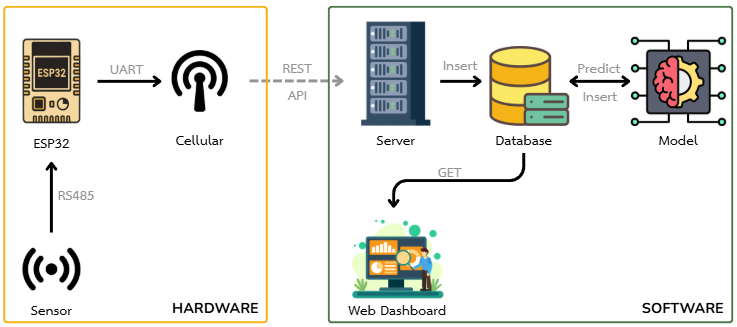
\includegraphics[width=0.7\textwidth]{images/chapter_3/overview.png} 
    \caption{แผนภาพแสดงการทำงานของระบบ}
    \label{fig:overview daigram}
\end{figure}

\section{สถานีวัดสภาพอากาศขนาดย่อม}
\subsection{โครงสร้างสถานีวัดสภาพอากาศขนาดย่อม}
\hspace{\parindent} โครงสร้างของสถานีวัดสภาพอากาศขนาดย่อมแบ่งเป็น 3 ส่วนหลัก คือ ระบบจ่ายไฟฟ้า, ชุดควบคุมหลัก และเซนเซอร์ตรวจวัดสภาพแวดล้อม 
โดยการเชื่อมต่อระหว่างชุดควบคุมหลักและเซนเซอร์ตรวจวัดสภาพแวดล้อมใช้การสื่อสารแบบ RS485 โดยการออกแบบจะเน้นไปที่การป้องกัน SPOF 
(Single Point of Failure), ซ่อมแซมง่าย, ประหยัดพลังงาน และเพิ่มความน่าเชื่อถือให้ระบบ
% Fix
\begin{figure}[H]
    \centering
    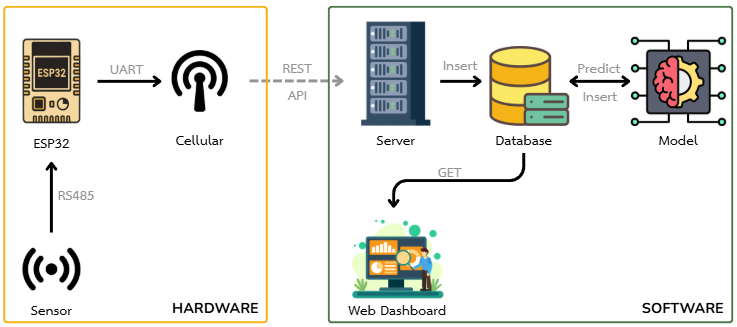
\includegraphics[width=0.7\textwidth]{images/chapter_3/overview.png} 
    \caption{แผนภาพแสดงการทำงานของระบบ}
    \label{fig:overview daigram}
\end{figure}

\subsection{อุปกรณ์ที่ใช้ในสถานีวัดสภาพอากาศขนาดย่อม}
\textbf{ระบบจ่ายไฟฟ้า} \\

\hspace{\parindent} ระบบใช้ไฟฟ้ากระแสตรงขนาด 12 โวลต์จากแหล่งจ่ายภายนอก และทำการแปลงแรงดันไฟฟ้าให้เหมาะสมกับอุปกรณ์แต่ละชนิด เช่น 5 โวลต์สำหรับไมโครคอนโทรลเลอร์ 
และ 3.3 โวลต์สำหรับเซนเซอร์บางประเภทโดยใช้โมดูล LM2596 และแหล่งจ่ายพลังงานสามารถปรับเปลี่ยนได้ตามสภาพแวดล้อมการติดตั้ง เช่น การใช้ระบบโซลาร์เซลล์หรืออะแดปเตอร์ไฟฟ้า 
ทั้งนี้การออกแบบระบบจ่ายไฟคำนึงถึงความเสถียรและการประหยัดพลังงานเป็นหลัก

\textbf{ชุดควบคุมหลัก}
% Fix
\begin{table}[h]
\centering
\begin{tabular}{|l|l|l|}
\hline
\textbf{อุปกรณ์} & \textbf{หน้าที่} & \textbf{การเชื่อมต่อ} \\ \hline
ESP32 & หน่วยควบคุมหลัก & - \\ \hline
SIMA7670E & ส่งข้อมูลไปที่ Server & UART \\ \hline
MAX485 & สื่อสารกับเซนเซอร์ผ่าน RS485 & RS485 \\ \hline
Relay Module & ควบคุมการจ่ายไฟฟ้าให้เซนเซอร์ & Digital (HIGH/LOW) \\ \hline
\end{tabular}
\caption{ตารางแสดงอุปกรณ์หลักในชุดควบคุมและการเชื่อมต่อ}
\label{tab:main control}
\end{table}

\hspace{\parindent} การเลือกใช้ RS485 ช่วยให้ระบบสามารถสื่อสารในระยะไกลและทนต่อสัญญาณรบกวนได้ดี เหมาะสำหรับการติดตั้งภายนอกอาคาร \\

\textbf{เซนเซอร์ตรวจวัดสภาพแวดล้อม}

\begin{table}[h]
\centering
\begin{tabular}{|l|l|c|l|}
\hline
\textbf{เซนเซอร์} & \textbf{หน้าที่} & \textbf{การเชื่อมต่อ} & \textbf{ความละเอียด} \\ \hline
\multirow{3}{*}{BME280} & วัดอุณหภูมิ & \multirow{3}{*}{I2C} & 0.01 $^\circ$C \\ \cline{2-2} \cline{4-4} 
 & วัดความชื้น &  & 0.008\% \\ \cline{2-2} \cline{4-4} 
 & วัดความกดอากาศ &  & 1 hPa \\ \hline
VEML7700 & วัดความเข้มแสง & I2C & 0.0036 Lux/CT \\ \hline
Wind Speed Sensor & วัดความเร็วลม & RS485 & 0.1 m/s \\ \hline
Wind Direction Sensor & วัดทิศทางลม & RS485 & 1$^\circ$ \\ \hline
PT100 & วัดอุณหภูมิ ณ จุดสัมผัส & RTD & 0.1 $^\circ$C \\ \hline
\end{tabular}
\caption{ตารางแสดงอุปกรณ์เซนเซอร์ที่ใช้ในสถานีวัดสภาพอากาศขนาดย่อม}
\label{tab:sensor list}
\end{table}

\hspace{\parindent} เซนเซอร์ที่ใช้การสื่อสารแบบ I2C และ RTD จะถูกแปลงสัญญาณเป็น RS485 เพื่อให้สามารถรวมอยู่ในระบบสื่อสารเดียวกัน ลดความซับซ้อนของระบบและเพิ่มความสามารถในการขยายในอนาคต \\

% Fix
\begin{figure}[H]
    \centering
    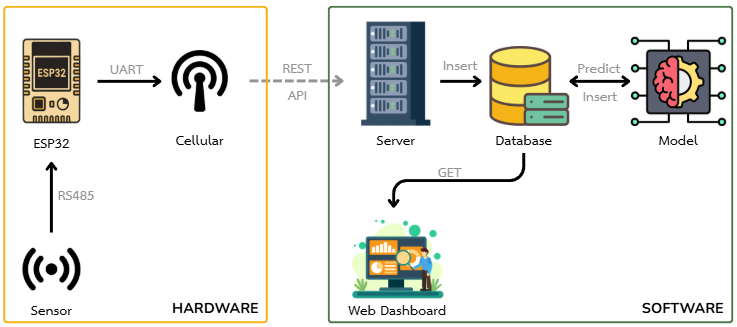
\includegraphics[width=0.7\textwidth]{images/chapter_3/overview.png} 
    \caption{แผนภาพแสดงการทำงานของระบบ}
    \label{fig:overview daigram}
\end{figure}

\begin{itemize}
    \item [] \textbf{3.1.2.1 การแปลงสัญญาณจาก I2C เป็น RS485 (I2C to RS485 Conversion)} \\ 
    \hspace{\parindent} จากตารางที่ \ref{tab:sensor list} จะเห็นว่าเซนเซอร์จำนวน 2 ตัว ได้แก่ BME280 และ VEML7700 ใช้การสื่อสารแบบ I2C ซึ่งเหมาะสำหรับการสื่อสารระยะสั้นภายในบอร์ดเดียวกัน 
    อย่างไรก็ตาม I2C มีข้อจำกัดด้านระยะทางและความทนทานต่อสัญญาณรบกวน จึงไม่เหมาะสมสำหรับการใช้งานในระบบที่ต้องติดตั้งเซนเซอร์ในระยะไกล
    \item [] \textbf{3.1.2.2 การแปลงสัญญาณจาก RTD เป็น RS485 (RTD to RS485 Conversion)} \\ 
    \hspace{\parindent} จากตารางที่ \ref{tab:sensor list} จะเห็นว่าเซนเซอร์ PT100 ที่ใช้ในการวัดอุณหภูมิ ณ บริเวณแผงโซลาร์เซลล์ ซึ่งเป็นเซนเซอร์ที่ทำงานโดยอาศัยการเปลี่ยนแปลงค่าความต้านทานตามอุณหภูมิ ซึ่งไม่สามารถเชื่อมต่อเข้ากับไมโครคอนโทรลเลอร์โดยตรงได้ จำเป็นต้องมีวงจรแปลงสัญญาณเพื่อแปลงค่าความต้านทานให้อยู่ในรูปแบบสัญญาณไฟฟ้าที่สามารถประมวลผลได้ \\
    
    \hspace{\parindent} ในการออกแบบระบบนี้ ได้มีการใช้โมดูลแปลงสัญญาณ RTD เป็น RS485 ซึ่งภายในโมดูลจะทำหน้าที่แปลงค่าความต้านทานของ PT100 ให้เป็นข้อมูลดิจิทัล และส่งออกผ่านการสื่อสารแบบ RS485 โดยใช้โปรโตคอล Modbus RTU ทำให้สามารถเชื่อมต่อเข้ากับระบบหลักได้โดยตรง \\
    กระบวนการทำงานของระบบสามารถอธิบายได้ดังนี้
    
    \begin{enumerate}
        \item โมดูล RTD ทำการวัดค่าความต้านทานจากเซนเซอร์ PT100
        \item แปลงค่าความต้านทานเป็นค่าอุณหภูมิด้วยวงจรภายใน
        \item จัดเก็บข้อมูลในรูปแบบรีจิสเตอร์ของ Modbus
        \item ส่งข้อมูลผ่าน RS485 เมื่อได้รับคำสั่งจากอุปกรณ์ Master
    \end{enumerate}
    
    \hspace{\parindent} การออกแบบลักษณะนี้ช่วยลดภาระการประมวลผลของไมโครคอนโทรลเลอร์ เนื่องจากการแปลงค่าทางกายภาพเป็นข้อมูลดิจิทัลถูกจัดการภายในโมดูลแล้ว อีกทั้งยังช่วยเพิ่มความแม่นยำของข้อมูล และลดความซับซ้อนในการออกแบบวงจร
    นอกจากนี้ การใช้การสื่อสารแบบ RS485 ยังช่วยให้สามารถติดตั้งเซนเซอร์ในระยะไกลได้ และมีความทนทานต่อสัญญาณรบกวน เหมาะสำหรับการใช้งานในสภาพแวดล้อมจริง

    \item [] \textbf{3.1.2.3 การสื่อสารข้อมูลด้วย RS485 และ Modbus RTU (RS485 and Modbus RTU Communication)} \\ 
    \hspace{\parindent} ภายในระบบสถานีวัดสภาพอากาศขนาดย่อม ได้เลือกใช้การสื่อสารแบบ RS485 ร่วมกับโปรโตคอล Modbus RTU เป็นกลไกหลักในการรับส่งข้อมูลระหว่างอุปกรณ์ต่าง ๆ เนื่องจาก RS485 มีความสามารถในการสื่อสารในระยะไกล และมีความทนทานต่อสัญญาณรบกวน เหมาะสำหรับการติดตั้งในสภาพแวดล้อมภายนอกอาคาร
    
    \hspace{\parindent} ในระบบนี้ โครงสร้างการสื่อสารออกแบบมาในลักษณะ Master-Slave โดยมีชุดควบคุมหลักทำหน้าที่เป็น Master และอุปกรณ์เซนเซอร์ทำหน้าที่เป็น Slave ซึ่งแต่ละอุปกรณ์จะมีหมายเลขประจำตัว (Slave ID) ดังนี้
    \begin{table}[h]
    \centering
    \begin{tabular}{|l|l|}
    \hline
    \textbf{อุปกรณ์} & \textbf{SlaveID} \\ \hline
    Wind Speed Sensor & 1 \\ \hline
    Wind Direction Sensor & 2 \\ \hline
    PT100 & 3 \\ \hline
    Sensor Node & 4 \\ \hline
    \end{tabular}
    \end{table}

    กระบวนการสื่อสารสามารถอธิบายได้ดังนี้
    \begin{enumerate}
        \item อุปกรณ์ Master ส่งคำสั่ง (Request) ไปยัง Slave ตามหมายเลข Slave ID
        \item Slave ที่ถูกเรียกจะตอบกลับข้อมูล (Response) ตามคำสั่งที่ได้รับ
        \item ข้อมูลจะถูกส่งในรูปแบบของเฟรมข้อมูลตามมาตรฐาน Modbus RTU
        \item Master ทำการรวบรวมข้อมูลจาก Slave หลายตัวเพื่อส่งไปยัง Server
    \end{enumerate}

    \hspace{\parindent} การออกแบบในลักษณะนี้ช่วยให้สามารถเชื่อมต่ออุปกรณ์หลายตัวบนสายสื่อสารเดียวกัน ลดจำนวนสายสัญญาณ และเพิ่มความสามารถในการขยายระบบในอนาคต \\
    \hspace{\parindent} นอกจากนี้ การใช้ Modbus RTU ซึ่งเป็นโปรโตคอลมาตรฐาน ยังช่วยให้สามารถรองรับอุปกรณ์จากผู้ผลิตที่หลากหลาย และเพิ่มความยืดหยุ่นในการพัฒนาระบบ

\end{itemize}

\subsection{หลักการทำงานของสถานีวัดสภาพอากาศขนาดย่อม}

\hspace{\parindent} สถานีวัดสภาพอากาศขนาดย่อมถูกออกแบบให้ทำงานในลักษณะของระบบกระจาย (Distributed System) โดยมีการสื่อสารระหว่างอุปกรณ์ผ่านเครือข่าย RS485 
และใช้โปรโตคอล Modbus RTU ในการรับส่งข้อมูล เพื่อรองรับการติดตั้งเซนเซอร์ในระยะไกลและเพิ่มความทนทานต่อสัญญาณรบกวน \\
% ใส่รูป
\hspace{\parindent} การทำงานของระบบสามารถแบ่งออกเป็น 3 ช่วงหลัก ได้แก่ การเริ่มต้นระบบ การตรวจสอบอุปกรณ์ และการเก็บข้อมูล โดยมีลำดับการทำงานดังนี้

\begin{enumerate}
    \item ขั้นตอนการเริ่มต้นระบบ (Initialization Phase)
    \begin{enumerate}
        \item ระบบจ่ายไฟให้กับชุดควบคุมหลัก
        \item ชุดควบคุมหลักทำการกำหนดค่าเริ่มต้นและตรวจสอบการเชื่อมต่อของอุปกรณ์ (Hardware Initialization)
    \end{enumerate}

    \item ขั้นตอนการตรวจสอบอุปกรณ์ (Device Checking Phase)
    \begin{enumerate}
        \item ชุดควบคุมหลักส่งคำสั่งไปยังอุปกรณ์แต่ละตัวเพื่อตรวจสอบสถานะการทำงาน
        \item อุปกรณ์ตอบกลับสถานะผ่านโปรโตคอล Modbus RTU
        \item ระบบส่งข้อมูลสถานะการทำงานของอุปกรณ์ไปยัง Server
        \item ระบบเข้าสู่โหมดประหยัดพลังงาน (Deep Sleep) เป็นระยะเวลา 15 นาที
        \item ทำซ้ำขั้นตอนที่ 3–6 เป็นจำนวน 4 รอบ เพื่อยืนยันความพร้อมของระบบก่อนเริ่มการเก็บข้อมูลจริง
    \end{enumerate}

    \item ขั้นตอนการเก็บและส่งข้อมูล (Data Acquisition Phase)
    \begin{enumerate}
        \item ชุดควบคุมหลักร้องขอข้อมูลจากเซนเซอร์ทั้งหมดผ่าน RS485
        \item เซนเซอร์ส่งค่าที่ตรวจวัดได้กลับมาในรูปแบบ Modbus Register
        \item ระบบทำการรวบรวมและจัดรูปแบบข้อมูล
        \item ส่งข้อมูลไปยัง Server ผ่านโมดูลสื่อสาร
        \item ระบบเข้าสู่โหมด Deep Sleep และวนกลับไปทำงานในขั้นตอนที่ 8
    \end{enumerate}
\end{enumerate}

\hspace{\parindent} การออกแบบลักษณะนี้ช่วยให้ระบบสามารถตรวจสอบความพร้อมของอุปกรณ์ก่อนเริ่มการทำงานจริง ลดความผิดพลาดในการเก็บข้อมูล และช่วยประหยัดพลังงานผ่านการใช้โหมด Deep Sleep อีกทั้งยังเพิ่มความน่าเชื่อถือของระบบโดยรวม

\section{โมเดลการทำนายการผลิตไฟฟ้าจากโซลาร์เซลล์}
\subsection{ภาพรวมของโมเดล (Model Overview)}
\subsection{ขั้นตอนการพัฒนาโมเดล (Model Development Process)}

\section{เซิฟเวอร์และเว็บไซต์สำหรับแสดงผล}
\subsection{ภาพรวมของระบบ (System Overview)}
\subsection{เทคโนโลยีและเครื่องมือที่ใช้ (Technology Stack and Tools)}
\subsection{การออกแบบฐานข้อมูลและการจัดการข้อมูล (Database Design and Data Management)}
\subsection{การออกแบบ API(Application Programming Interface)}
\subsection{การออกแบบส่วนติดต่อผู้ใช้และเว็บไซต์ (Frontend and User Interface Design)}
\chapter{\ifproject%
\ifenglish Experimentation and Results\else การทดลองและผลลัพธ์\fi
\else%
\ifenglish System Evaluation\else การประเมินระบบ\fi
\fi}
\section{สถานีวัดสภาพอากาศขนาดย่อม}
   \hspace{\parindent} สถานีวัดสภาพอากาศขนาดย่อม อุปกรณ์ฮาร์ดแวร์จะต้องถูกนำมาประกอบและติดตั้งรวมกันไว้ภายในกล่องกันน้ำ เพื่อจัดระเบียบสายไฟและป้องกันความเสียหายจากสภาพแวดล้อมภายนอก เช่น ความชื้น ฝน และความร้อน ซึ่งทำให้ระบบพร้อมสำหรับการนำไปติดตั้งในพื้นที่หน้างานจริง 
   โดยภายในสถานีประกอบด้วยชุดเซ็นเซอร์หลักที่ทำหน้าที่ตรวจวัดและรวบรวมตัวแปรทางสภาพอากาศที่สำคัญ ได้แก่ เซ็นเซอร์ BME280 สำหรับวัดอุณหภูมิ ความชื้น และความกดอากาศ, เซ็นเซอร์ VEML7700 สำหรับวัดปริมาณความเข้มแสงแดด, เซ็นเซอร์ Wind Speed สำหรับวัดวัดความเร็ว, เซ็นเซอร์ Wind Direction สำหรับวัดทิศทางลม และเซ็นเซอร์ PT100 สำหรับวัดอุณหภูมิใต้แผงโซลาร์เซลล์ 
   \begin{figure}[H]
        \centering
        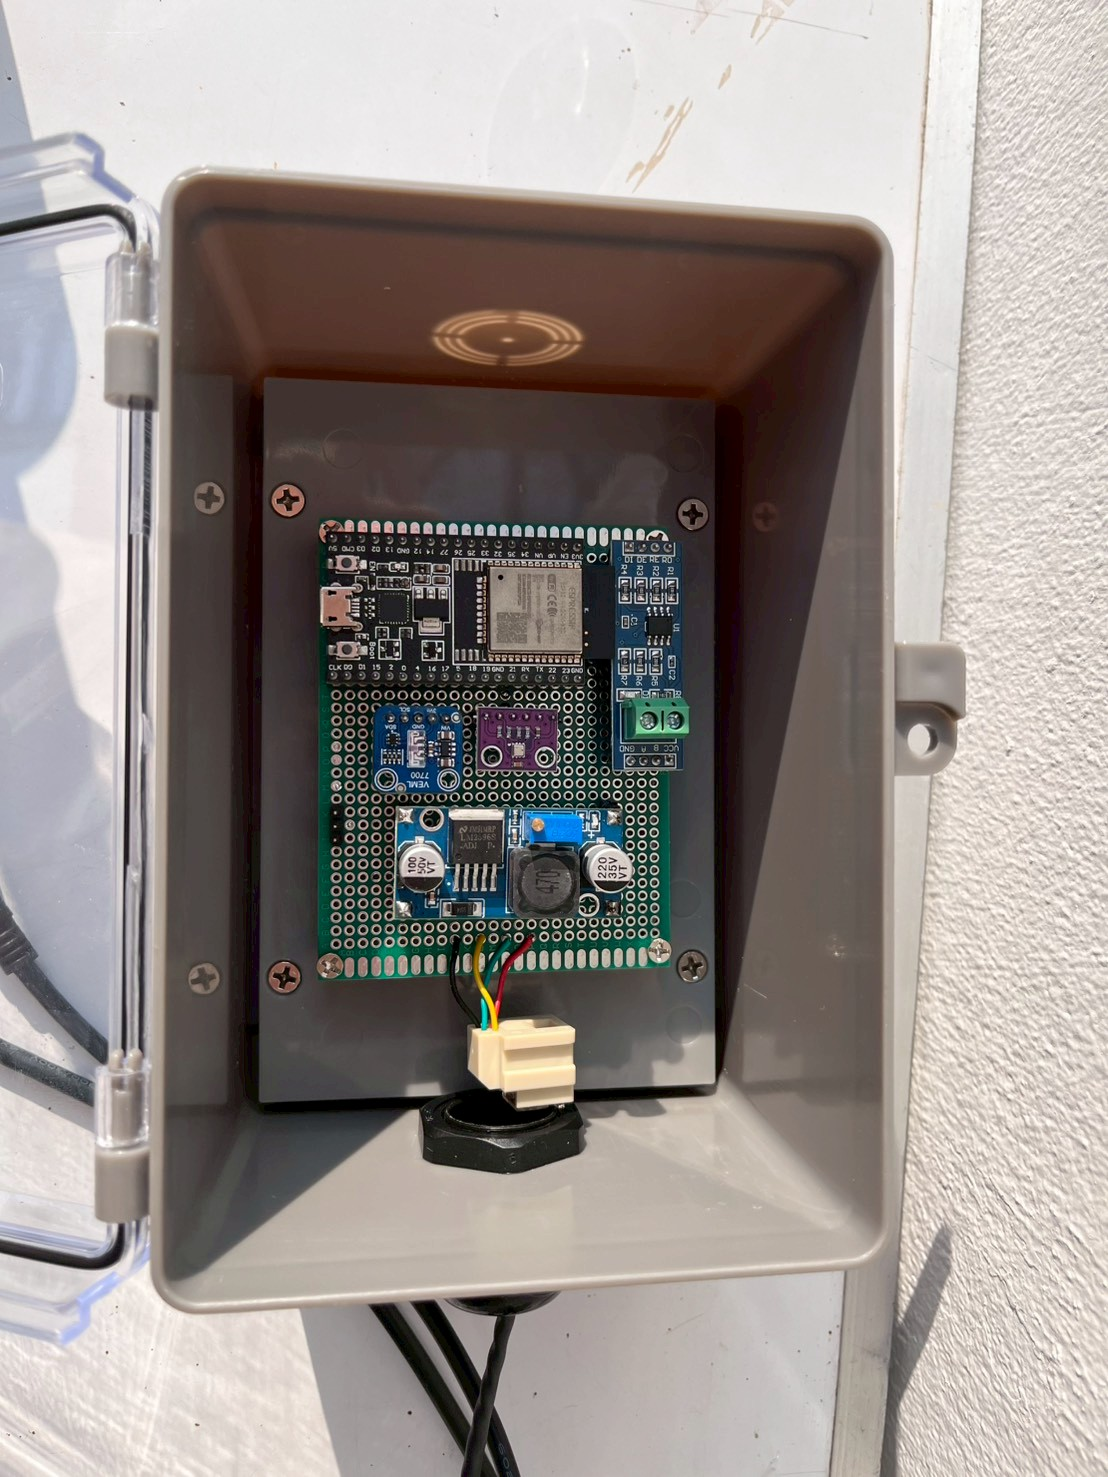
\includegraphics[width=0.7\textwidth, angle=90]{images/chapter_3/LINE_ALBUM_Station_260322_1.jpg}
        \caption{เซ็นเซอร์ BME280 และ VEML7700}
        \label{fig:BME280_VEML7700}
    \end{figure} 
    \begin{figure}[H]
        \centering
        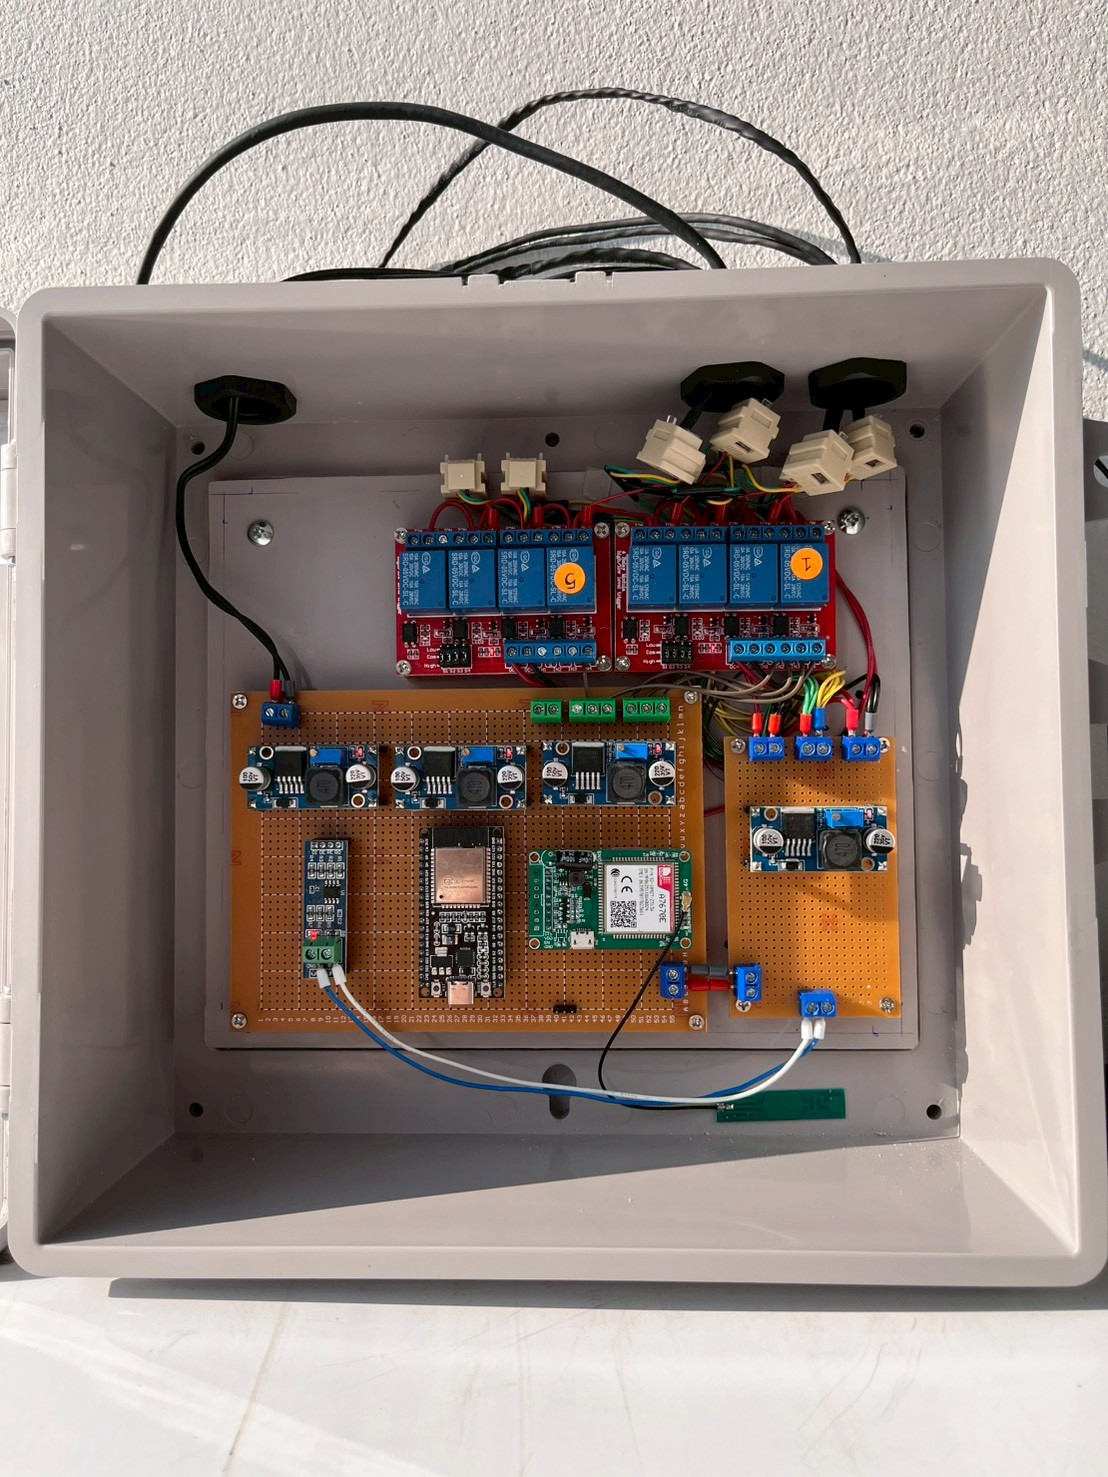
\includegraphics[width=0.7\textwidth]{images/chapter_3/main_result.jpg}
        \caption{เซ็นเซอร์ Wind Speed Wind, Direction และ PT100}
        \label{fig:Wind Speed Wind, Direction และ PT100}
    \end{figure}
     \begin{figure}[H]
        \centering
        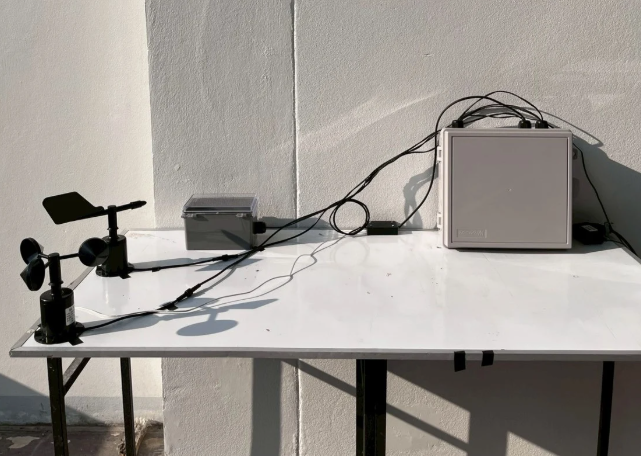
\includegraphics[width=0.7\textwidth]{picture/Hardware overview.png}
        \caption{ภาพรวมของสถานีวัดสภาพอากาศขนาดย่อม}
        \label{fig:Hardware overview}
    \end{figure}

\section{Web Dashboard}
\begin{itemize}
    \item[]\textbf{4.2.1 หน้าจอหลัก (Home)} ประกอบไปด้วยเมนู 2 เมนูคือ
    \begin{itemize}
        \item Station: เลือกสถานีวัดสภาพอากาศขนาดย่อมที่ต้องการดูข้อมูล
        \item Setting Station: เมนูสำหรับเจ้าหน้าที่ที่สามารถเข้าไปเช็คสถานะการทำงานของสถานีวัดสภาพอากาศขนาดย่อม
    \end{itemize}
    \begin{figure}[H]
        \centering
        \includegraphics[width=0.7\textwidth]{images/home.jpg}
        \caption{หน้าจอแสดงผลหลัก}
        \label{fig:Home}
    \end{figure}
    \begin{figure}[H]
        \centering
        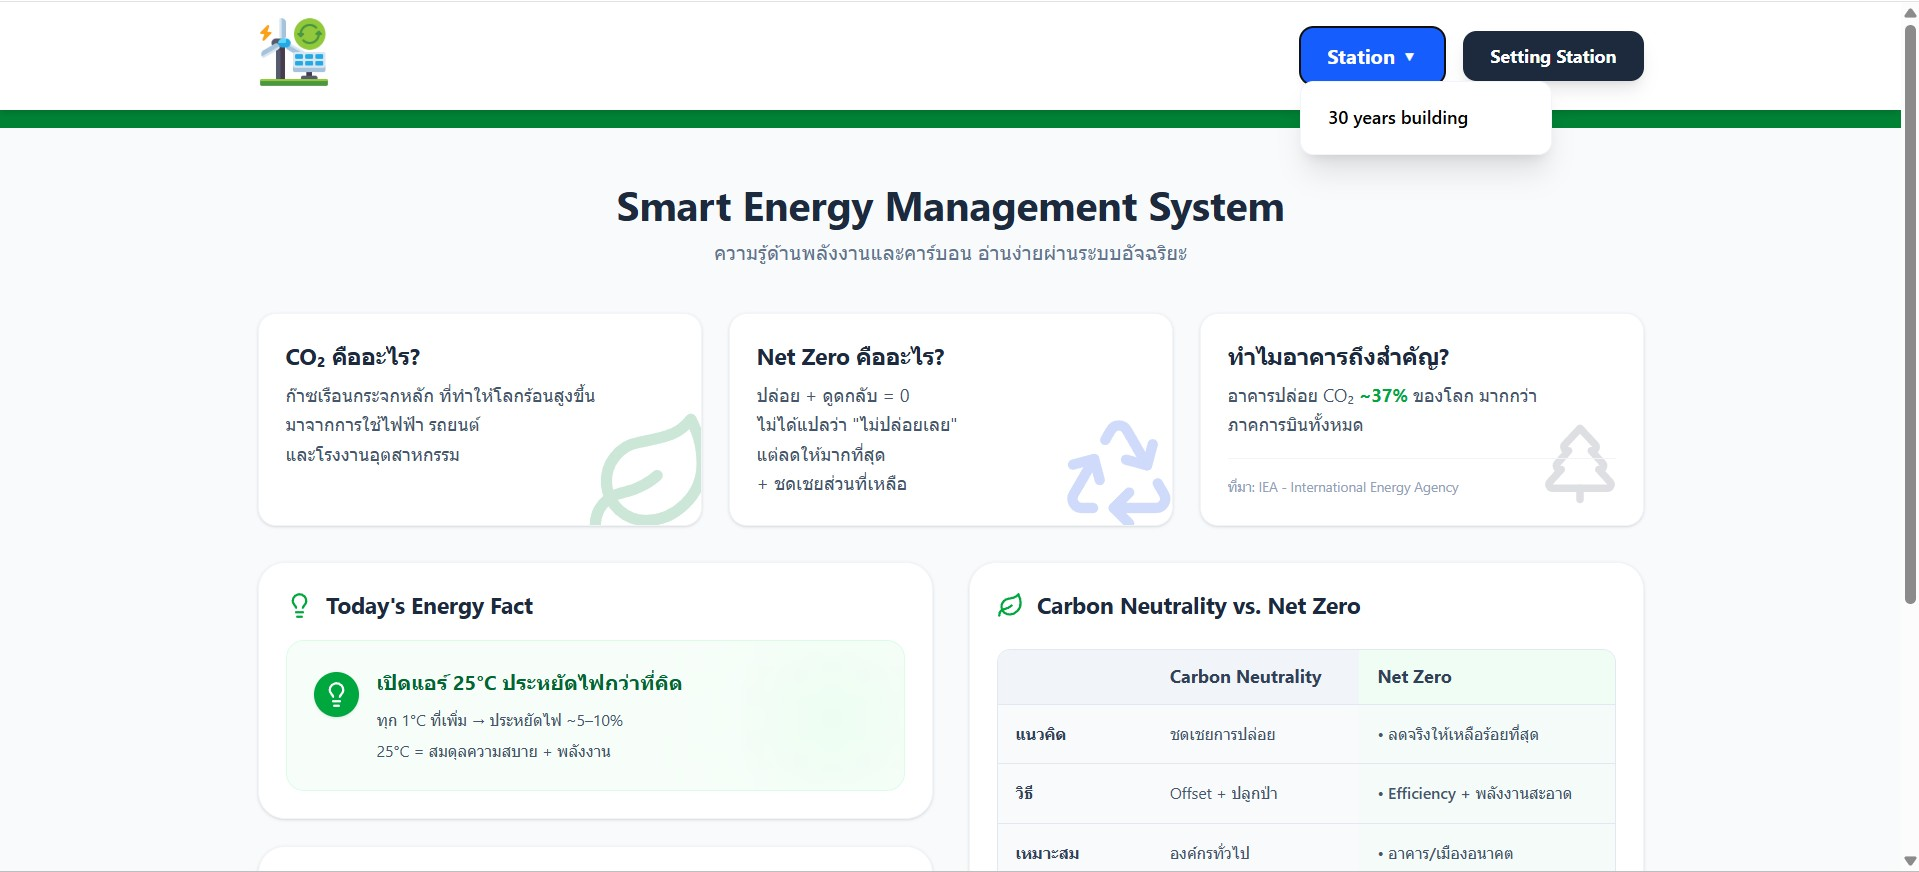
\includegraphics[width=0.7\textwidth]{images/select_station.jpg}
        \caption{หน้าจอการแสดงผลเมื่อผู้ใช้คลิกปุ่ม Station}
        \label{fig:select menu}
    \end{figure}

    \item[]\textbf{4.2.2 หน้าเมนู} หน้านี้จะแสดงข้อมูลทั้งหมดของระบบหลังจากที่ผู้ใช้เลือกปุ่ม Station ซึ่งประกอบไปด้วย
    \begin{itemize}
        \item เมนู Electric Current: แสดงกราฟการพยากรณ์ปริมาณการผลิตไฟฟ้าจากแผงโซลาร์เซลล์ซึ่งผู้ใช้สามารถเลือกวันที่ที่ต้องการดูข้อมูลได้
        \item เมนู Sunlight VS Solar Temp , Temp $&$ Humidity, Pressure, Wind Speed, Wind Direction เป็นเมนูแสดงข้อมูลที่ถูกส่งมาจากสถานีวัดสภาพอากาศขนาดย่อมรายชั่วโมง
    \end{itemize}
    \begin{figure}[H]
        \centering
        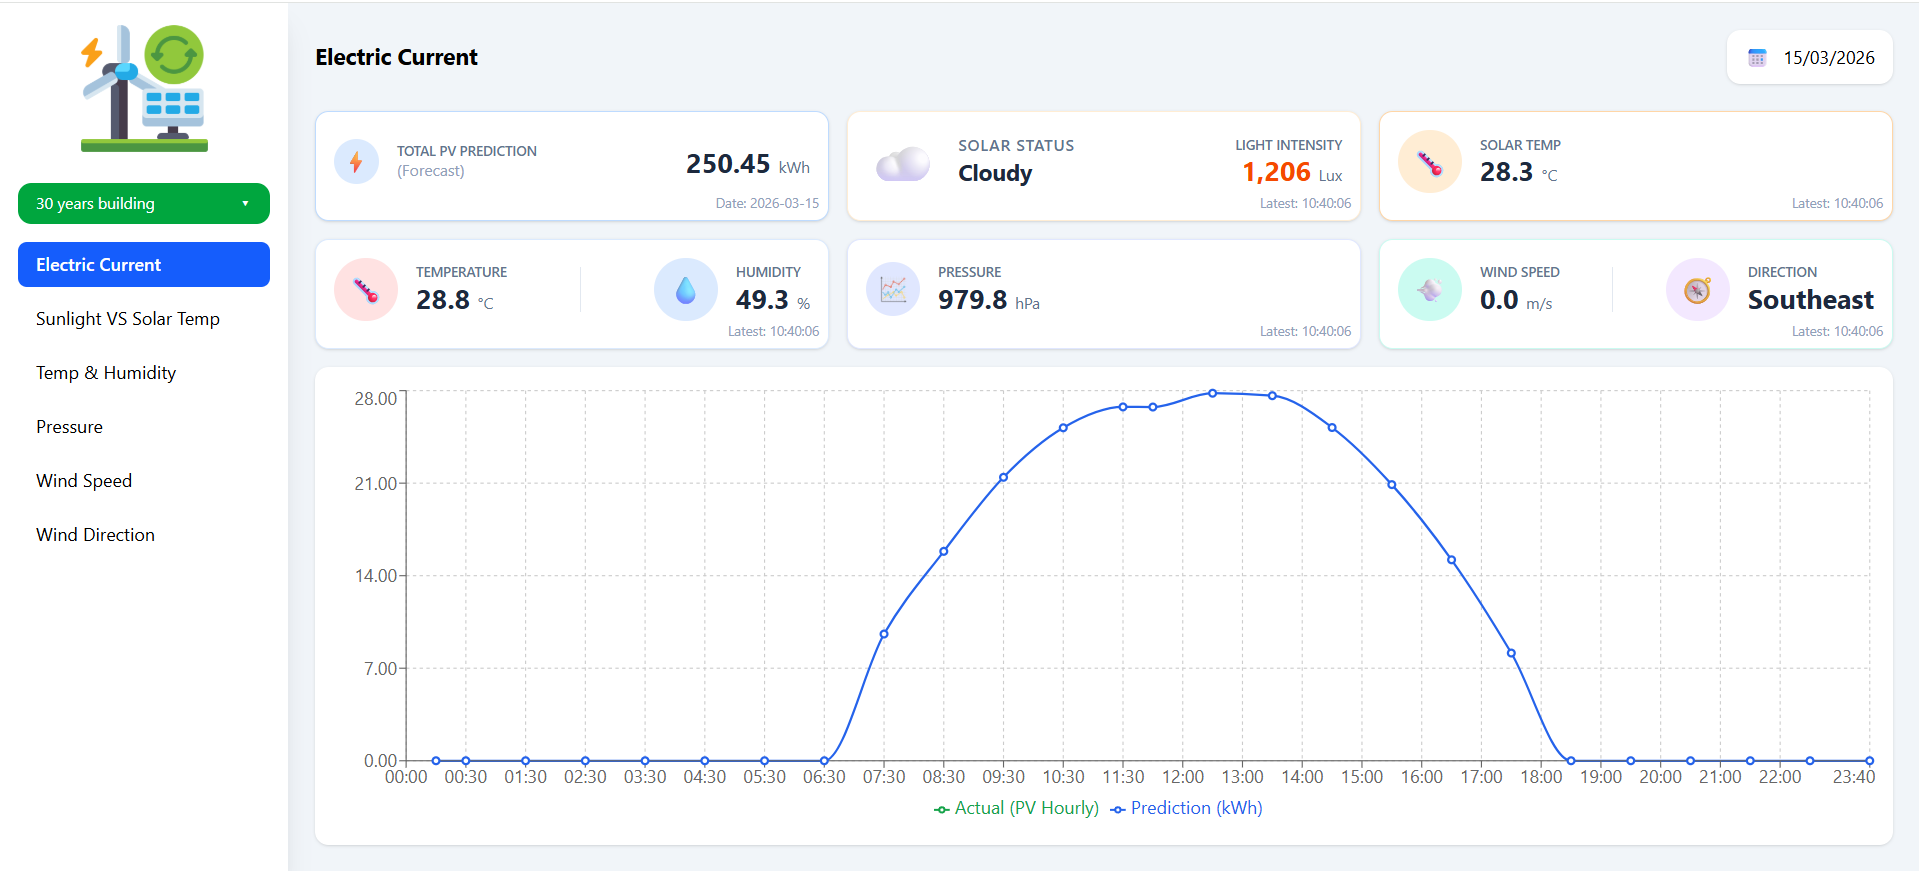
\includegraphics[width=0.7\textwidth]{images/predicgraph.png}
        \caption{หน้าจอแสดงข้อมูลสภาพอากาศและกราฟการพยากรณ์ปริมาณการผลิตไฟฟ้าจากโซลาร์เซลล์ล่วงหน้า 24 ชั่วโมง}
        \label{fig:Pradicgraph}
    \end{figure}
    \begin{figure}[H]
        \centering
        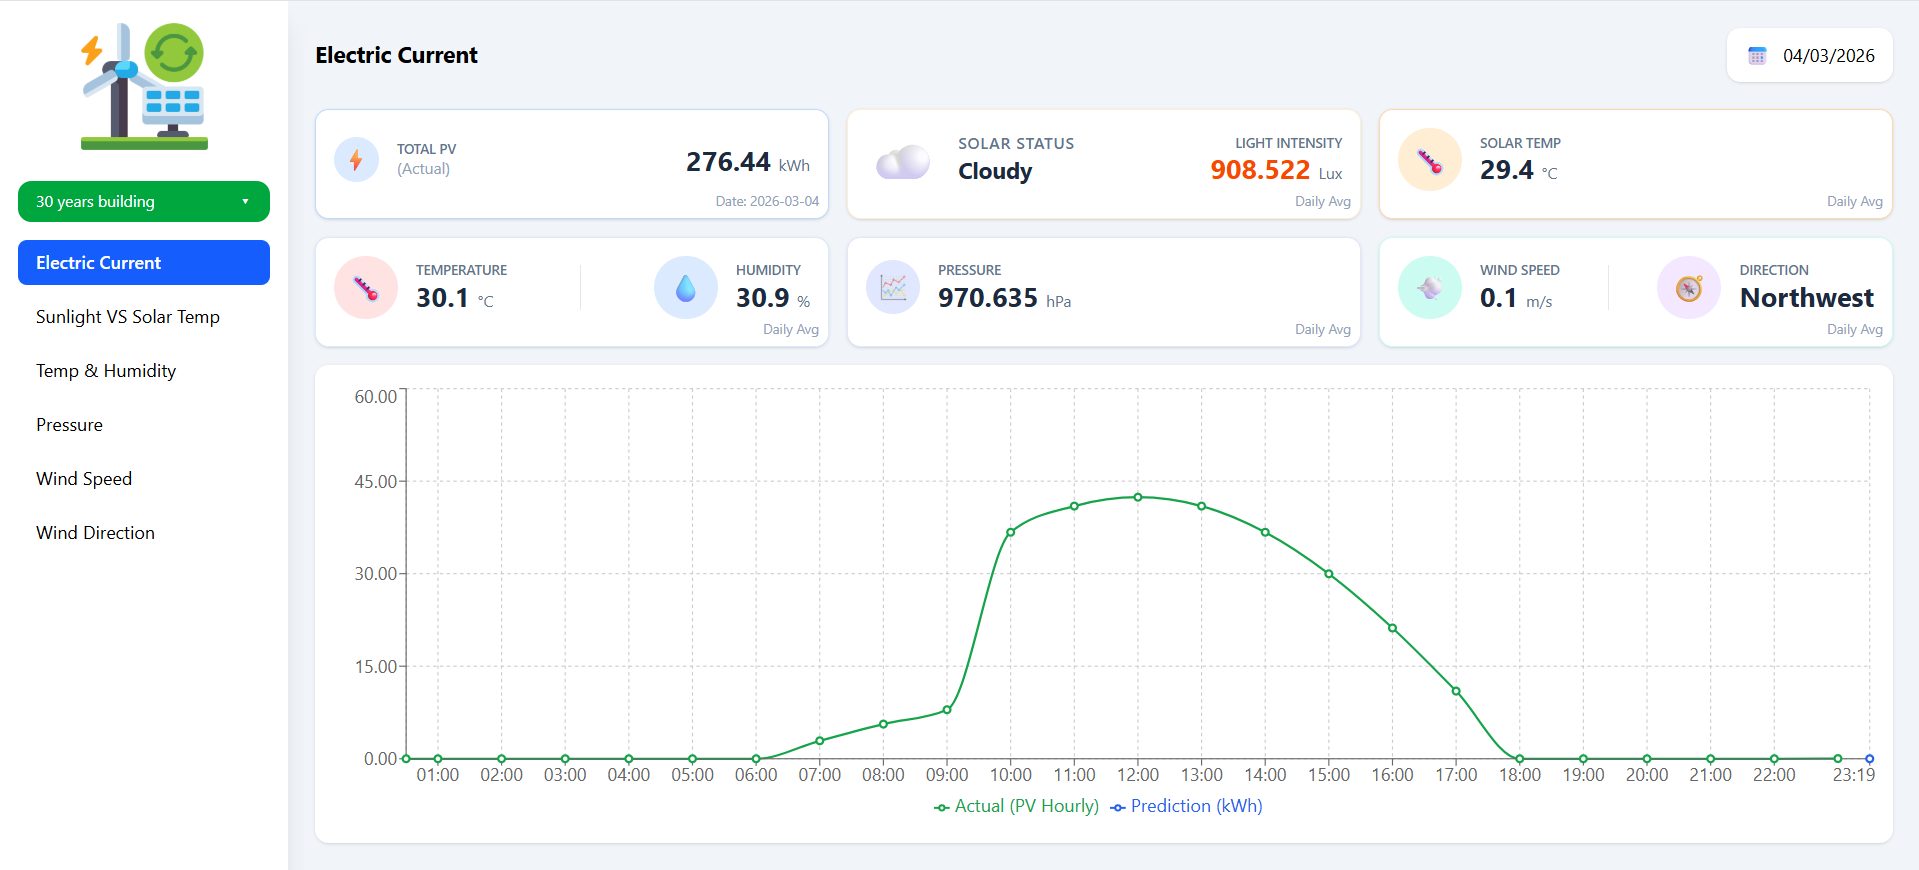
\includegraphics[width=0.7\textwidth]{images/actualgraph.png}
        \caption{หน้าจอแสดงผลเมื่อผู้ใช้เลือกเมนู Electric Current}
        \label{fig:Electric Current}
    \end{figure}
    \begin{figure}[H]
        \centering
        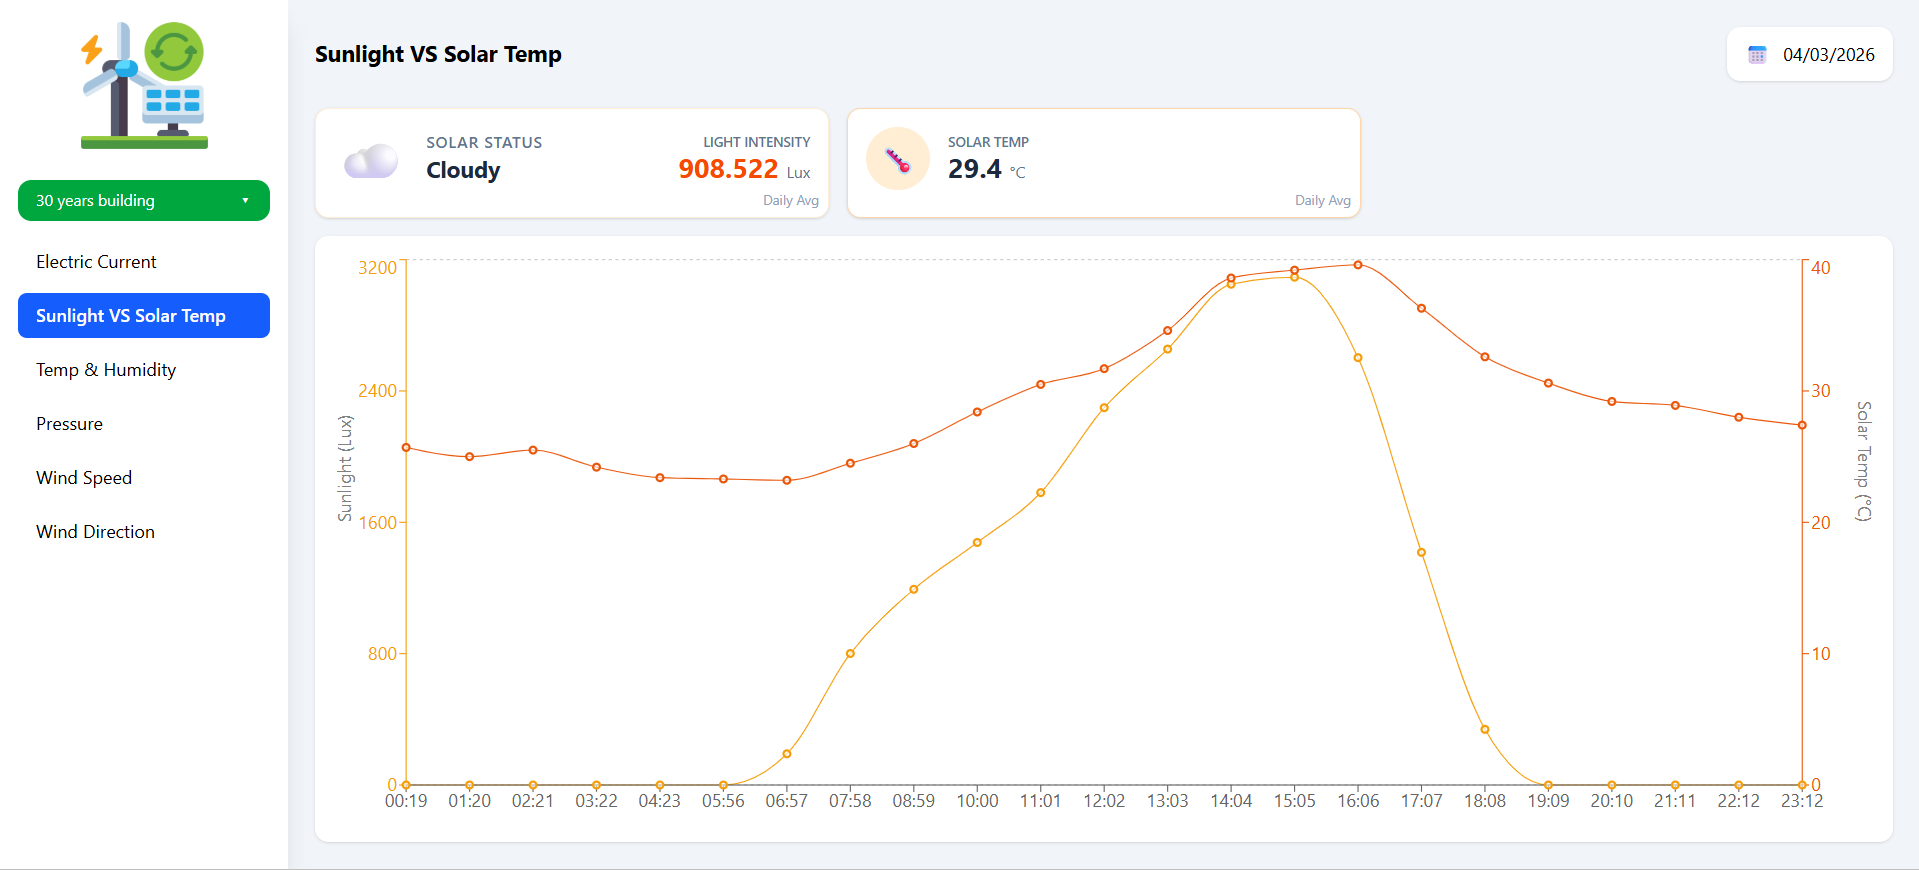
\includegraphics[width=0.7\textwidth]{images/sunlightandsolar.png}
        \caption{หน้าจอแสดงผลเมื่อผู้ใช้เลือกเมนู Sunlight VS Solar Temp}
        \label{fig:Sunlight VS Solar Temp}
    \end{figure}
    \begin{figure}[H]
        \centering
        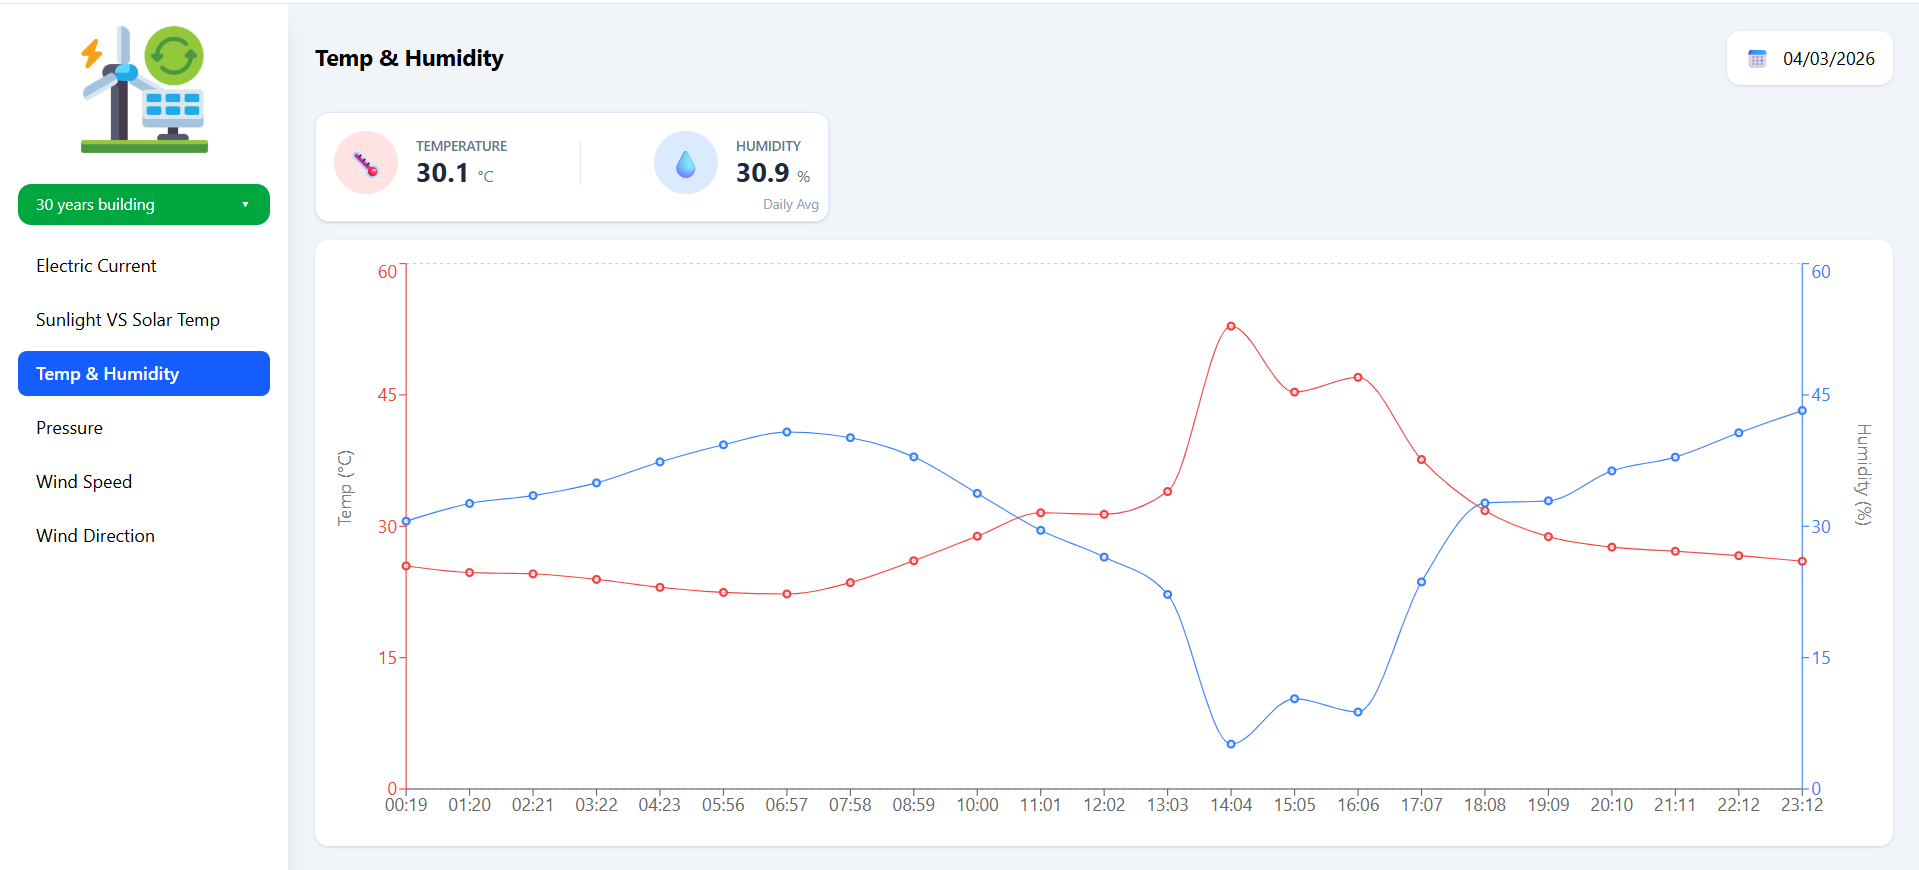
\includegraphics[width=0.7\textwidth]{images/tempandhum.png}
        \caption{หน้าจอแสดงผลเมื่อผู้ใช้เลือกเมนู Temp $&$ Humidity}
        \label{fig:Temp and Humidity}
    \end{figure}
    \begin{figure}[H]
        \centering
        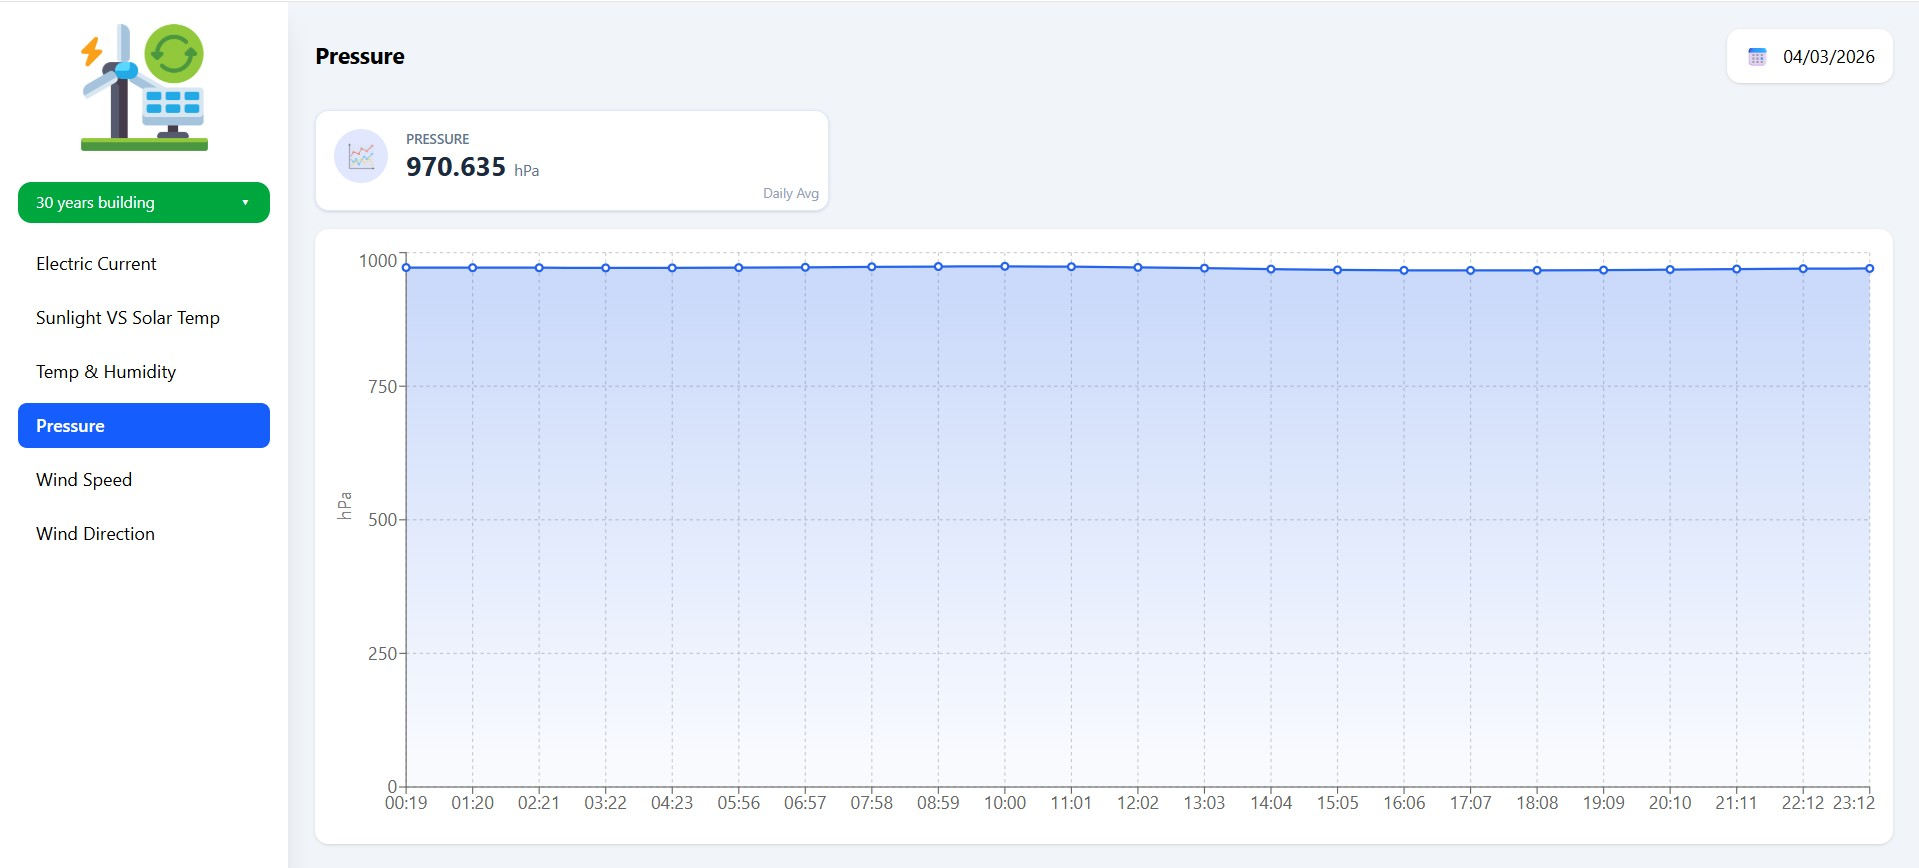
\includegraphics[width=0.7\textwidth]{images/pressure.jpg}
        \caption{หน้าจอแสดงผลเมื่อผู้ใช้เลือกเมนู Pressure}
        \label{fig:Pressure}
    \end{figure}
    \begin{figure}[H]
        \centering
        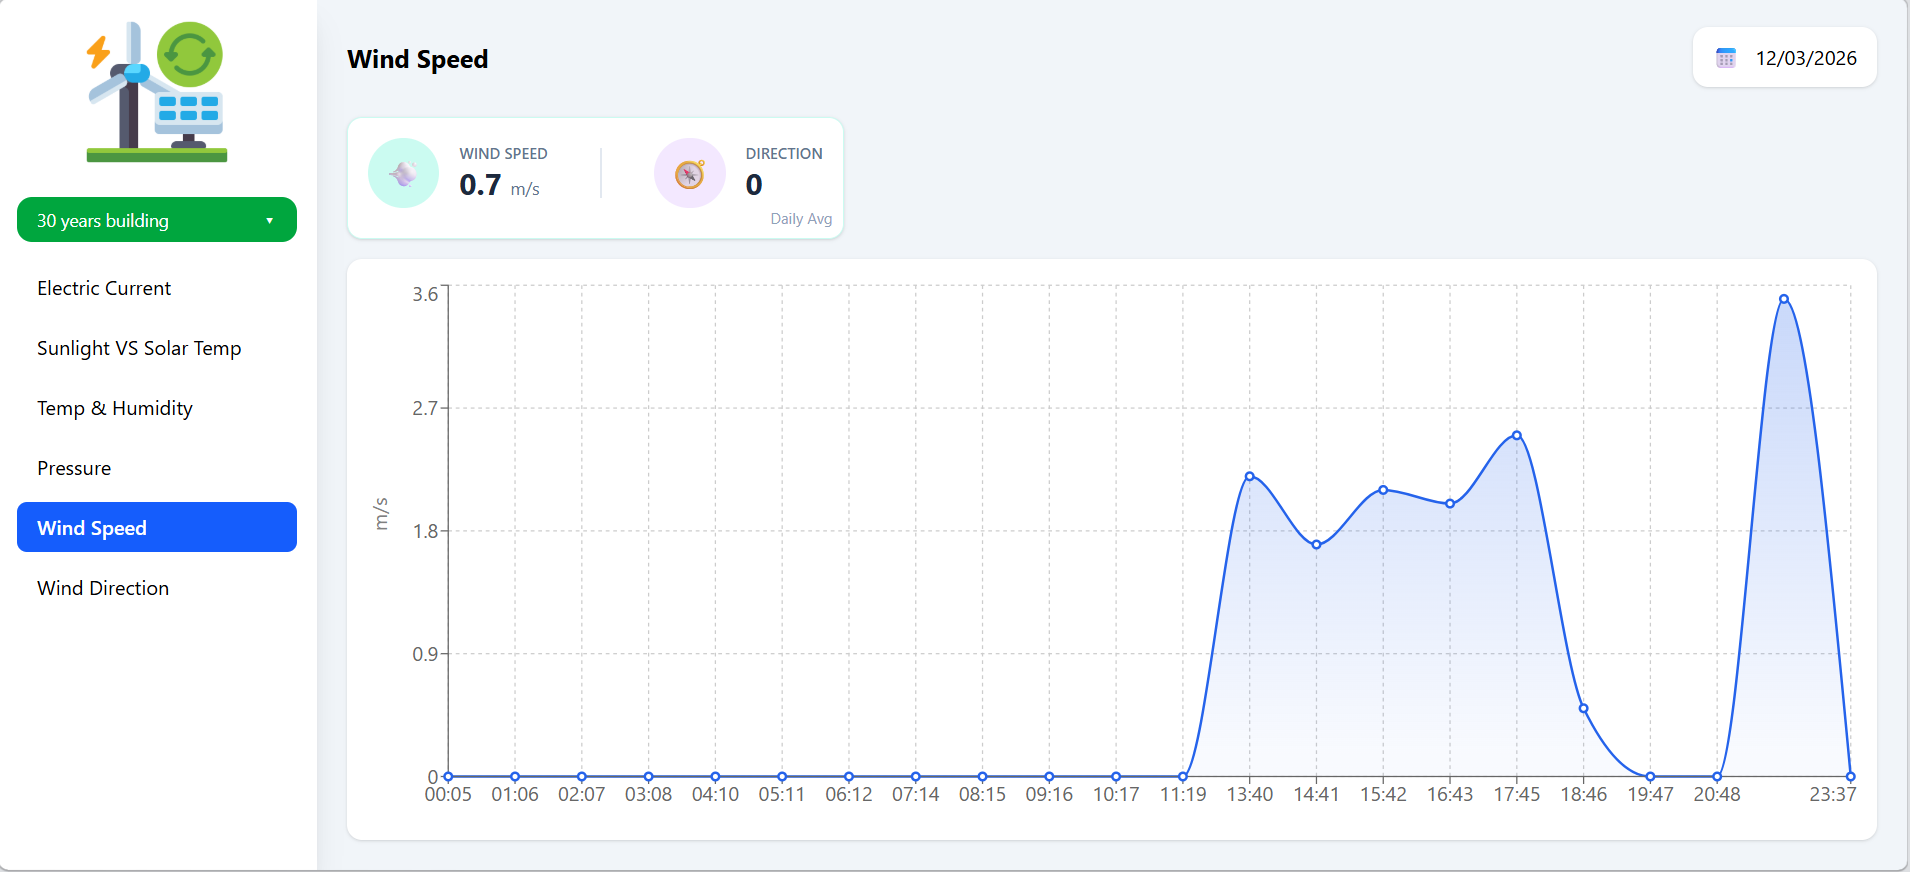
\includegraphics[width=0.7\textwidth]{picture/Wind Speed.png}
        \caption{หน้าจอแสดงผลเมื่อผู้ใช้เลือกเมนู Wind Speed}
        \label{fig:Wind Speed}
    \end{figure}
    \begin{figure}[H]
        \centering
        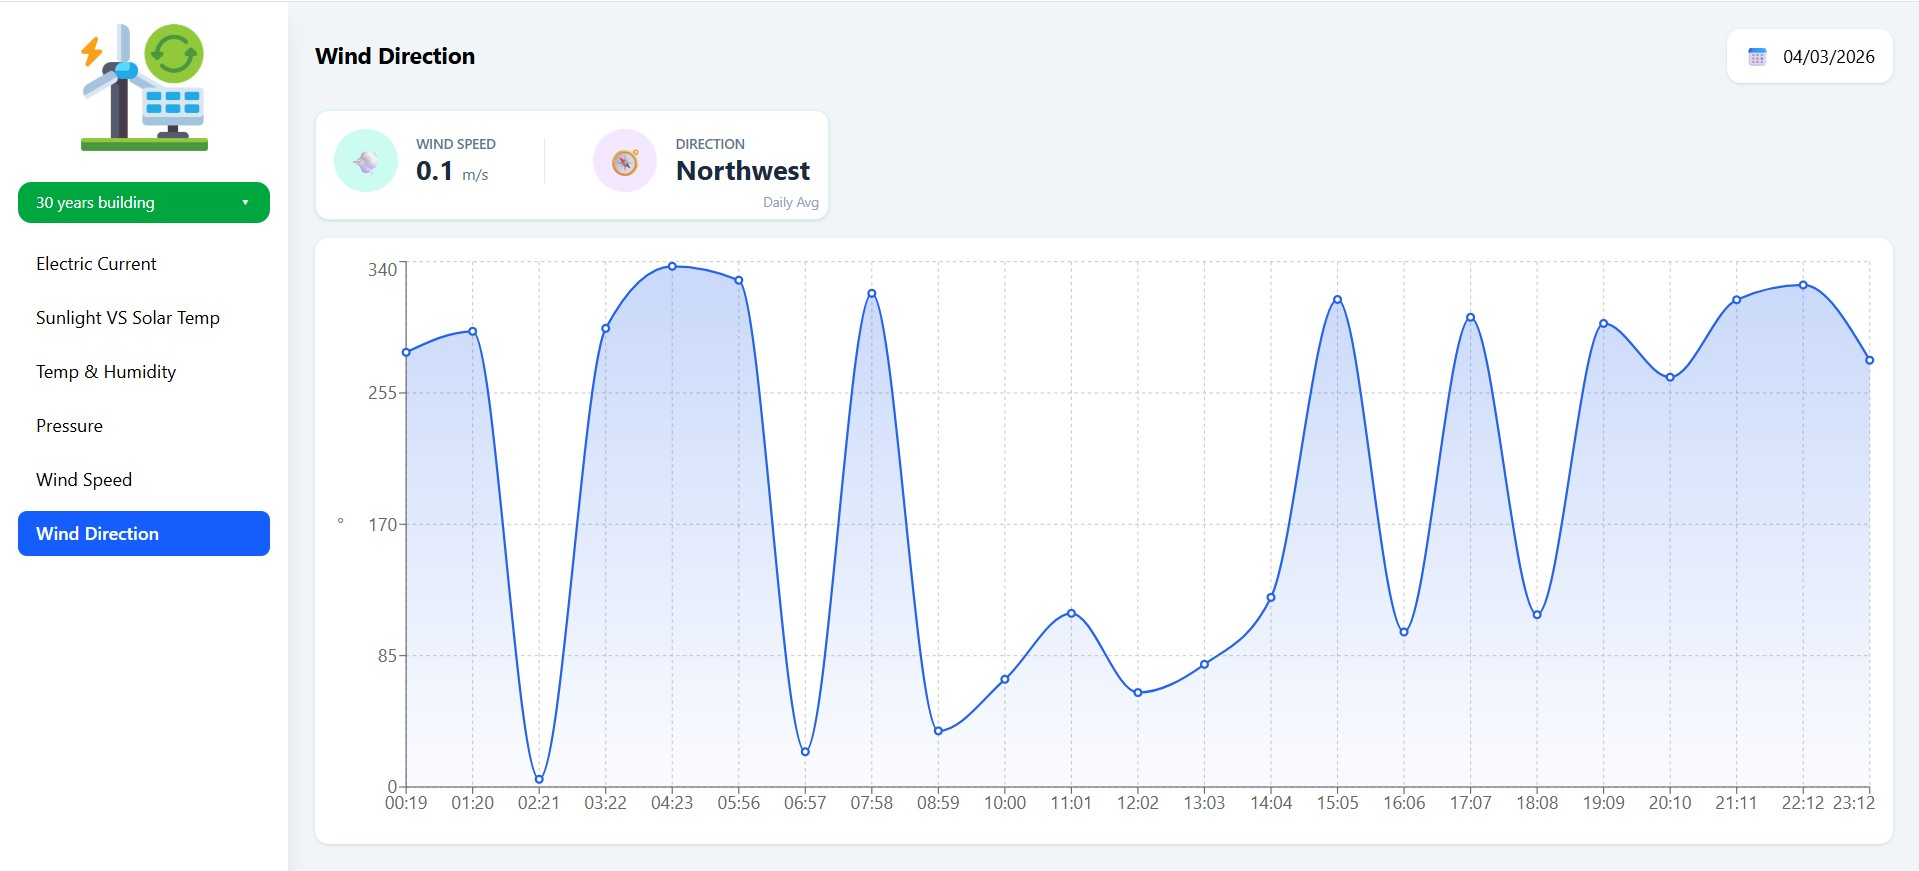
\includegraphics[width=0.7\textwidth]{images/winddirection.jpg}
        \caption{หน้าจอแสดงผลเมื่อผู้ใช้เลือกเมนู Wind Direction}
        \label{fig:Wind Direction}
    \end{figure}

    \item[]\textbf{4.2.3 หน้าสำหรับเข้าสู่ระบบ (Login)} หน้านี้มีขึ้นมาเพื่อให้เจ้าหน้าที่เท่านั้นที่สามารถเข้าถึงการทำงานของสถานีวัดสภาพอากาศขนาดย่อมเท่านั้น
    \begin{figure}[H]
        \centering
        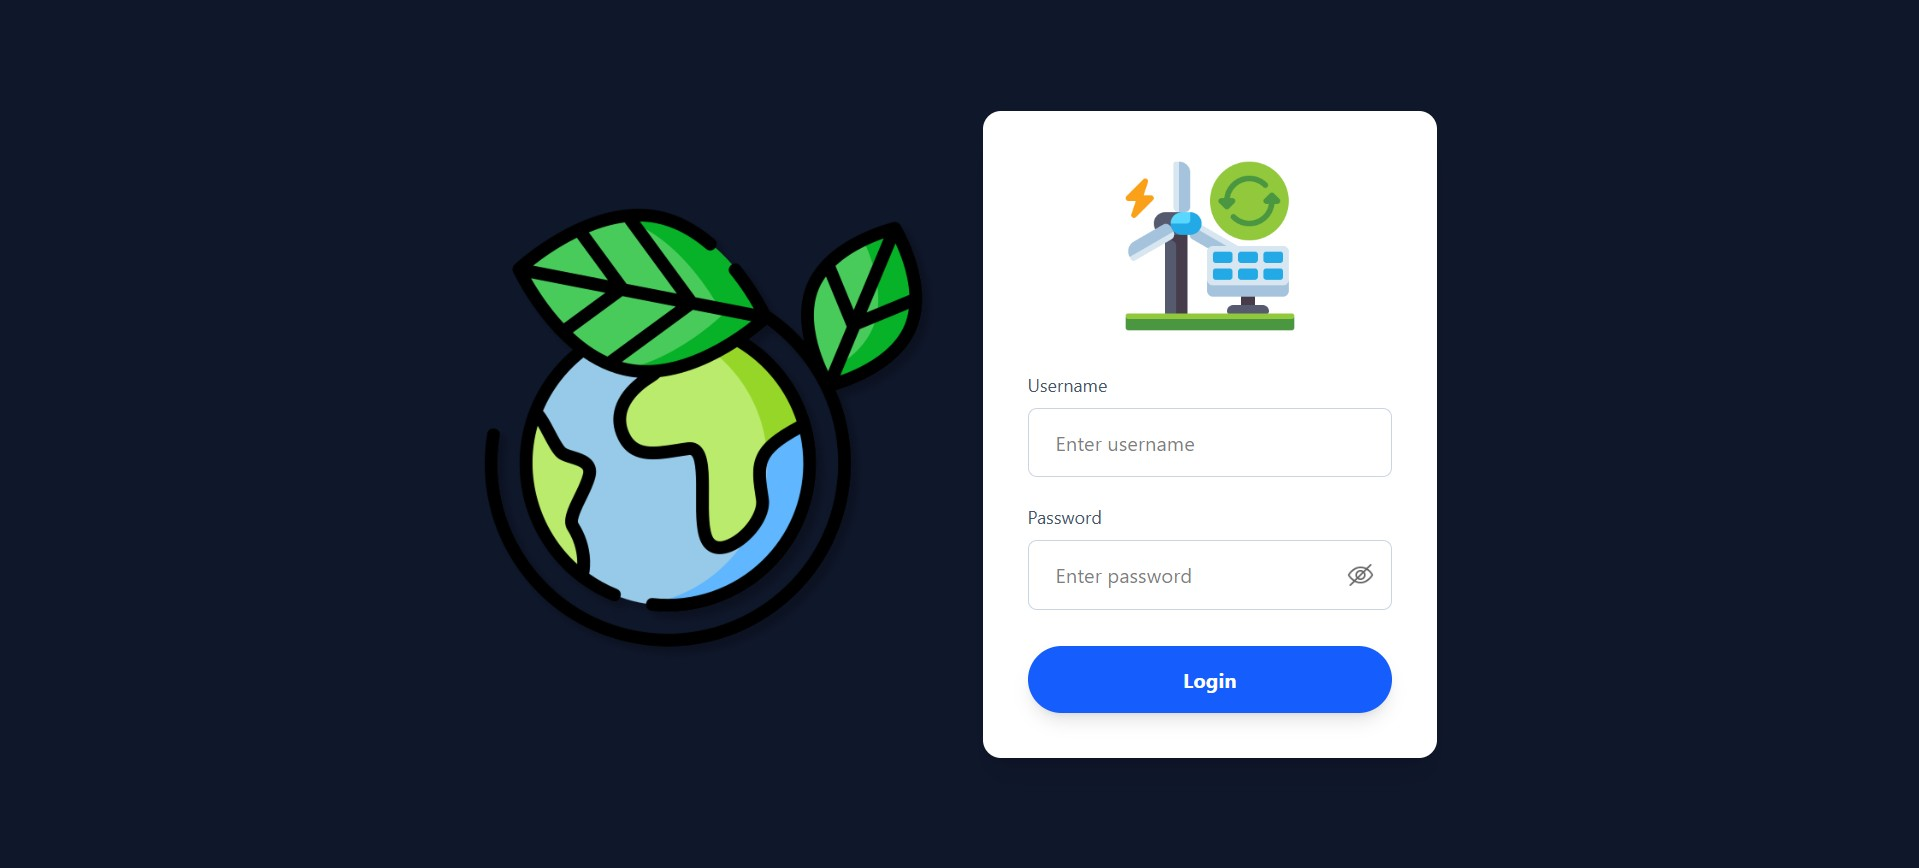
\includegraphics[width=0.7\textwidth]{images/login.jpg}
        \caption{หน้าแสดงผลเมื่อผู้ใช้เลือกเมนู Setting Station}
        \label{fig:Login}
    \end{figure}

    \item[]\textbf{4.2.4 หน้าแสดงสถานะ Status Sensor} หน้านี้มีขึ้นเพื่อติดตามสถานะการทำงานของตัววัดสถานีสภาพอากาศขนาดย่อมโดยสถานีจะต้องส่งสถานะมาทุกๆ 15 นาทีและเจ้าหน้าที่จะต้องสามารถติดตามสถานะของเซนเซอร์แต่ละตัวได้
    \begin{figure}[H]
        \centering
        
\includegraphics[width=0.7\textwidth]{statusstationOK.png} 
        \caption{สถานะการทำงานของสถานีวัดสภาพอากาศขนาดย่อมทำงานปกติ}
        \label{fig:statusstationOK}
        \end{figure}
    \begin{figure}[H]
        \centering
        
\includegraphics[width=0.7\textwidth]{statusstationNG.png} 
        \caption{สถานะการทำงานของสถานีวัดสภาพอากาศขนาดย่อมทำงานผิดปกติ}
        \label{fig:statusstationNG}
        \end{figure}
\end{itemize}

\subsection{การวิเคราะห์กราฟ Actual vs Predicted}

\begin{figure}[H]
    \centering
    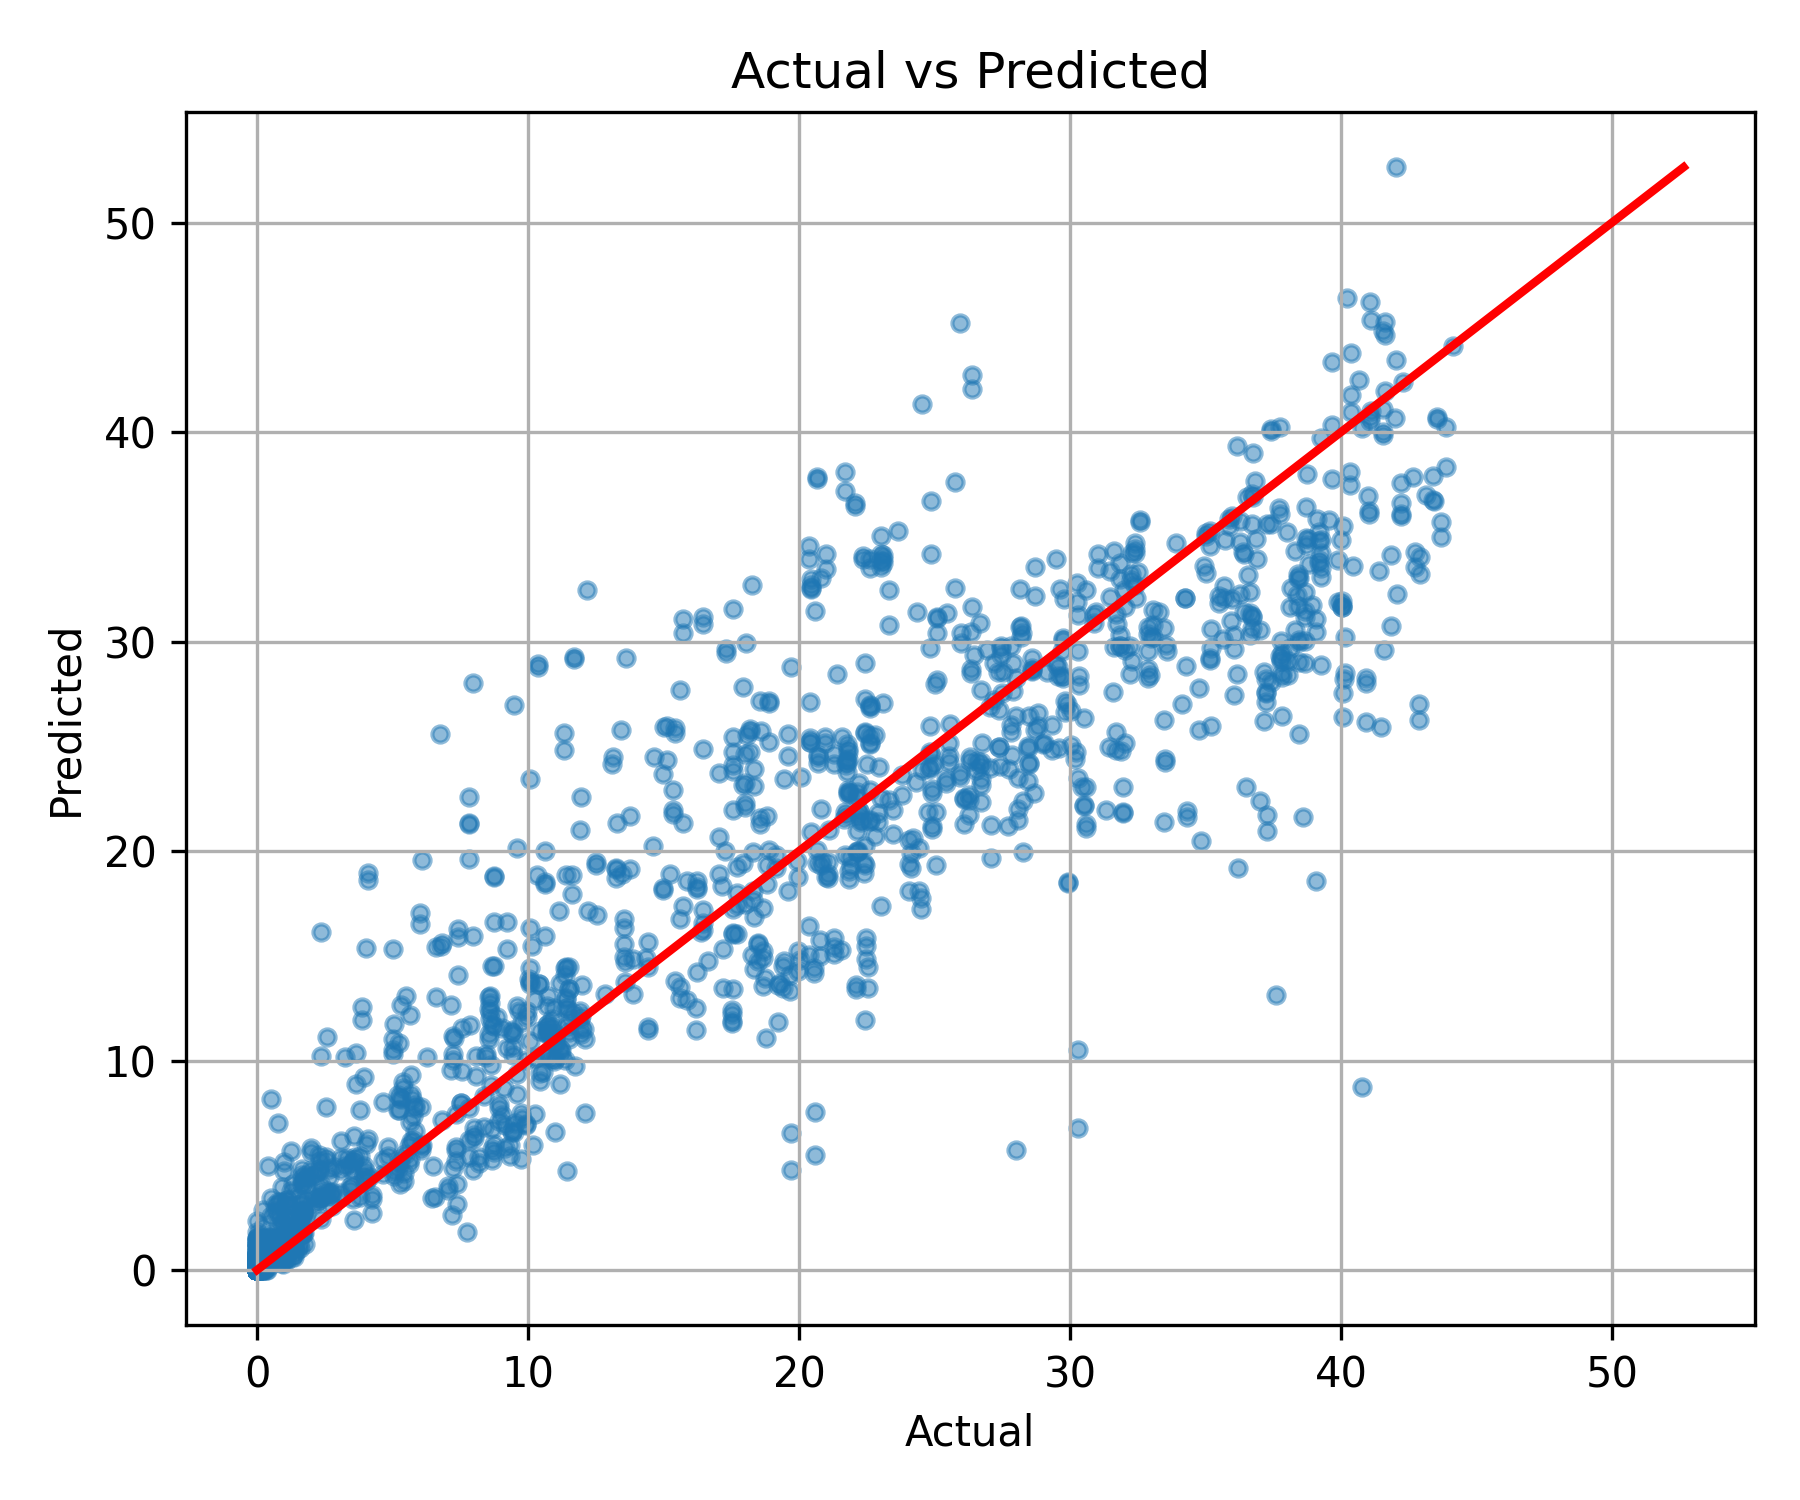
\includegraphics[width=0.7\textwidth]{picture/2_actual_vs_predicted.png}
    \caption[กราฟ Actual vs Predicted]{กราฟ Actual vs Predicted}
    \label{fig:image1}
\end{figure}

\vspace{10pt}
\begin{flushleft}
\hspace*{0.5cm}
จากกราฟเปรียบเทียบค่า Actual และ Prediction โดยแกน x คือ Actual และ แกน y คือ Prediction โดยพบว่าค่าการทำนายมีความสอดคล้องกับค่าจริงในภาพรวม โดยจุดข้อมูลส่วนใหญ่กระจายตัวใกล้กับเส้นทแยงมุมสีแดง แสดงให้เห็นว่าโมเดลสามารถเรียนรู้ความสัมพันธ์ระหว่างตัวแปรสภาพอากาศกับการผลิตไฟฟ้าจากโซลาร์เซลล์ได้อย่างมีประสิทธิภาพ 
อย่างไรก็ตาม ในช่วงค่าการผลิตไฟฟ้าสูง จะพบการกระจายตัวของจุดข้อมูลเพิ่มขึ้น ซึ่งสะท้อนให้เห็นว่าความคลาดเคลื่อนของโมเดลมีแนวโน้มเพิ่มขึ้นเมื่อกำลังผลิตสูงขึ้น อาจเกิดจากความผันผวนของสภาพอากาศแบบฉับพลัน เช่น เมฆบังแดด หรือการเปลี่ยนแปลงของอุณหภูมิที่รวดเร็ว
\end{flushleft}



\subsection{การวิเคราะห์ Residual Plot}

\begin{figure}[H]
    \centering
    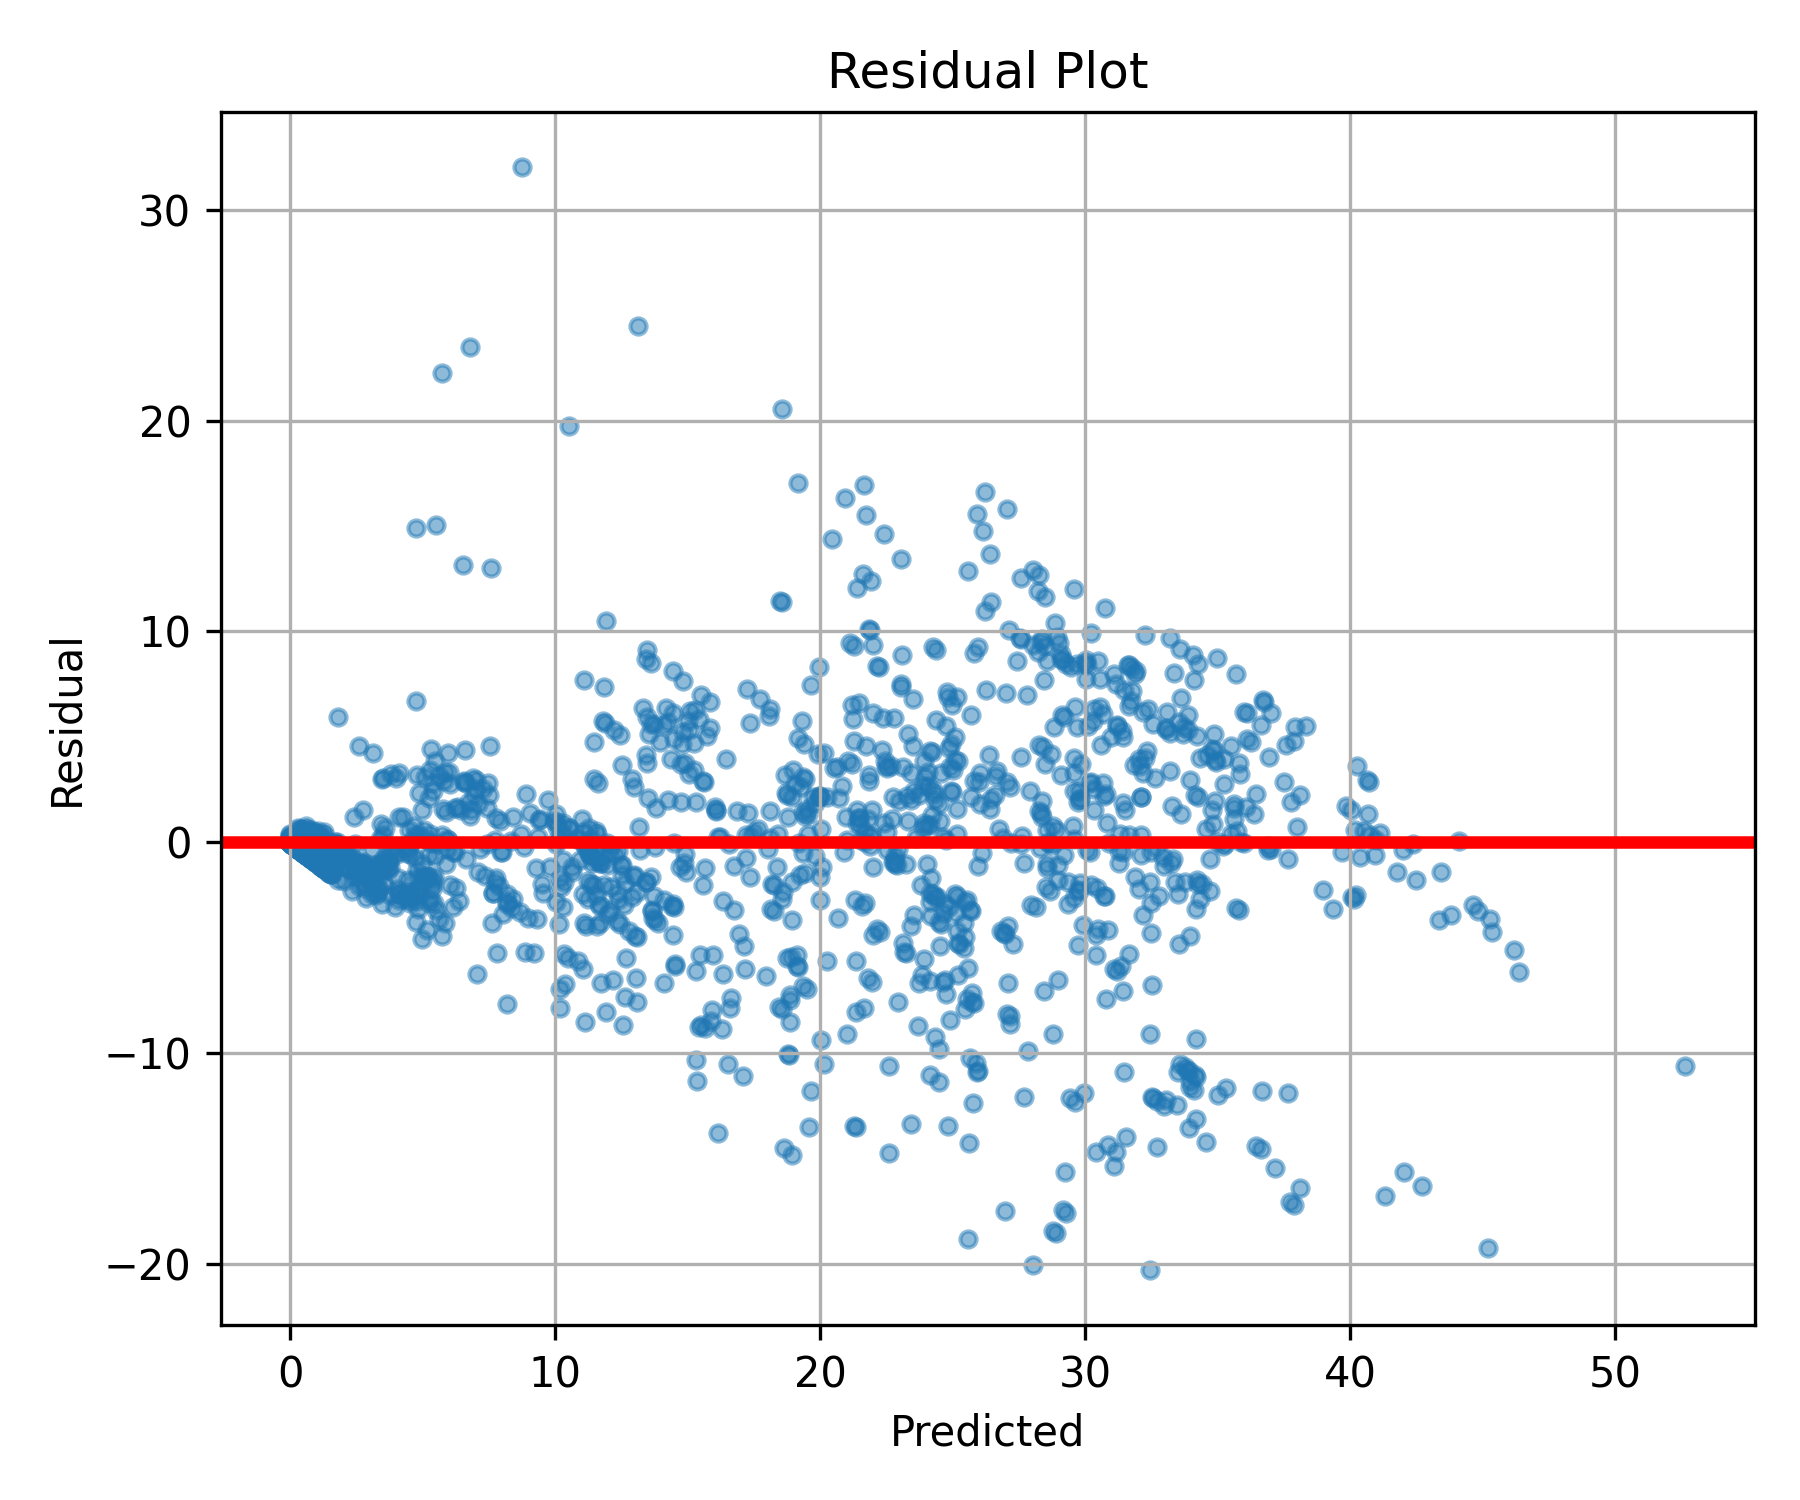
\includegraphics[width=0.7\textwidth]{picture/3_residual_plot.png}
    \caption[Residual Plot]{Residual Plot}
    \label{fig:image2}
\end{figure}

\vspace{10pt}
\begin{flushleft}
\hspace*{0.5cm}
จากกราฟจะพบว่าค่าความคลาดเคลื่อนส่วนใหญ่กระจายอยู่รอบค่า 0 แสดงว่าโมเดลไม่มีแนวโน้มทำนายค่าสูงเกินจริง หรือ ต่ำเกินจริง อย่างไรก็ตาม จะเห็นว่าการกระจายของ residual มีลักษณะขยายตัวมากขึ้นเมื่อค่าที่ทำนายมีค่าสูง ซึ่งแสดงถึงความแปรปรวนของความคลาดเคลื่อนที่เพิ่มขึ้นตามระดับกำลังผลิตไฟฟ้า 
อาจเป็นผลมาจากปัจจัยภายนอกที่มีผลต่อการผลิตไฟฟ้าในช่วงเวลานั้น เช่น สภาพอากาศที่ไม่คงที่ หรือข้อจำกัดของชุดข้อมูลในการฝึกฝนโมเดล
\end{flushleft}



\subsection{การวิเคราะห์ Feature Importance}

\begin{figure}[H]
    \centering
    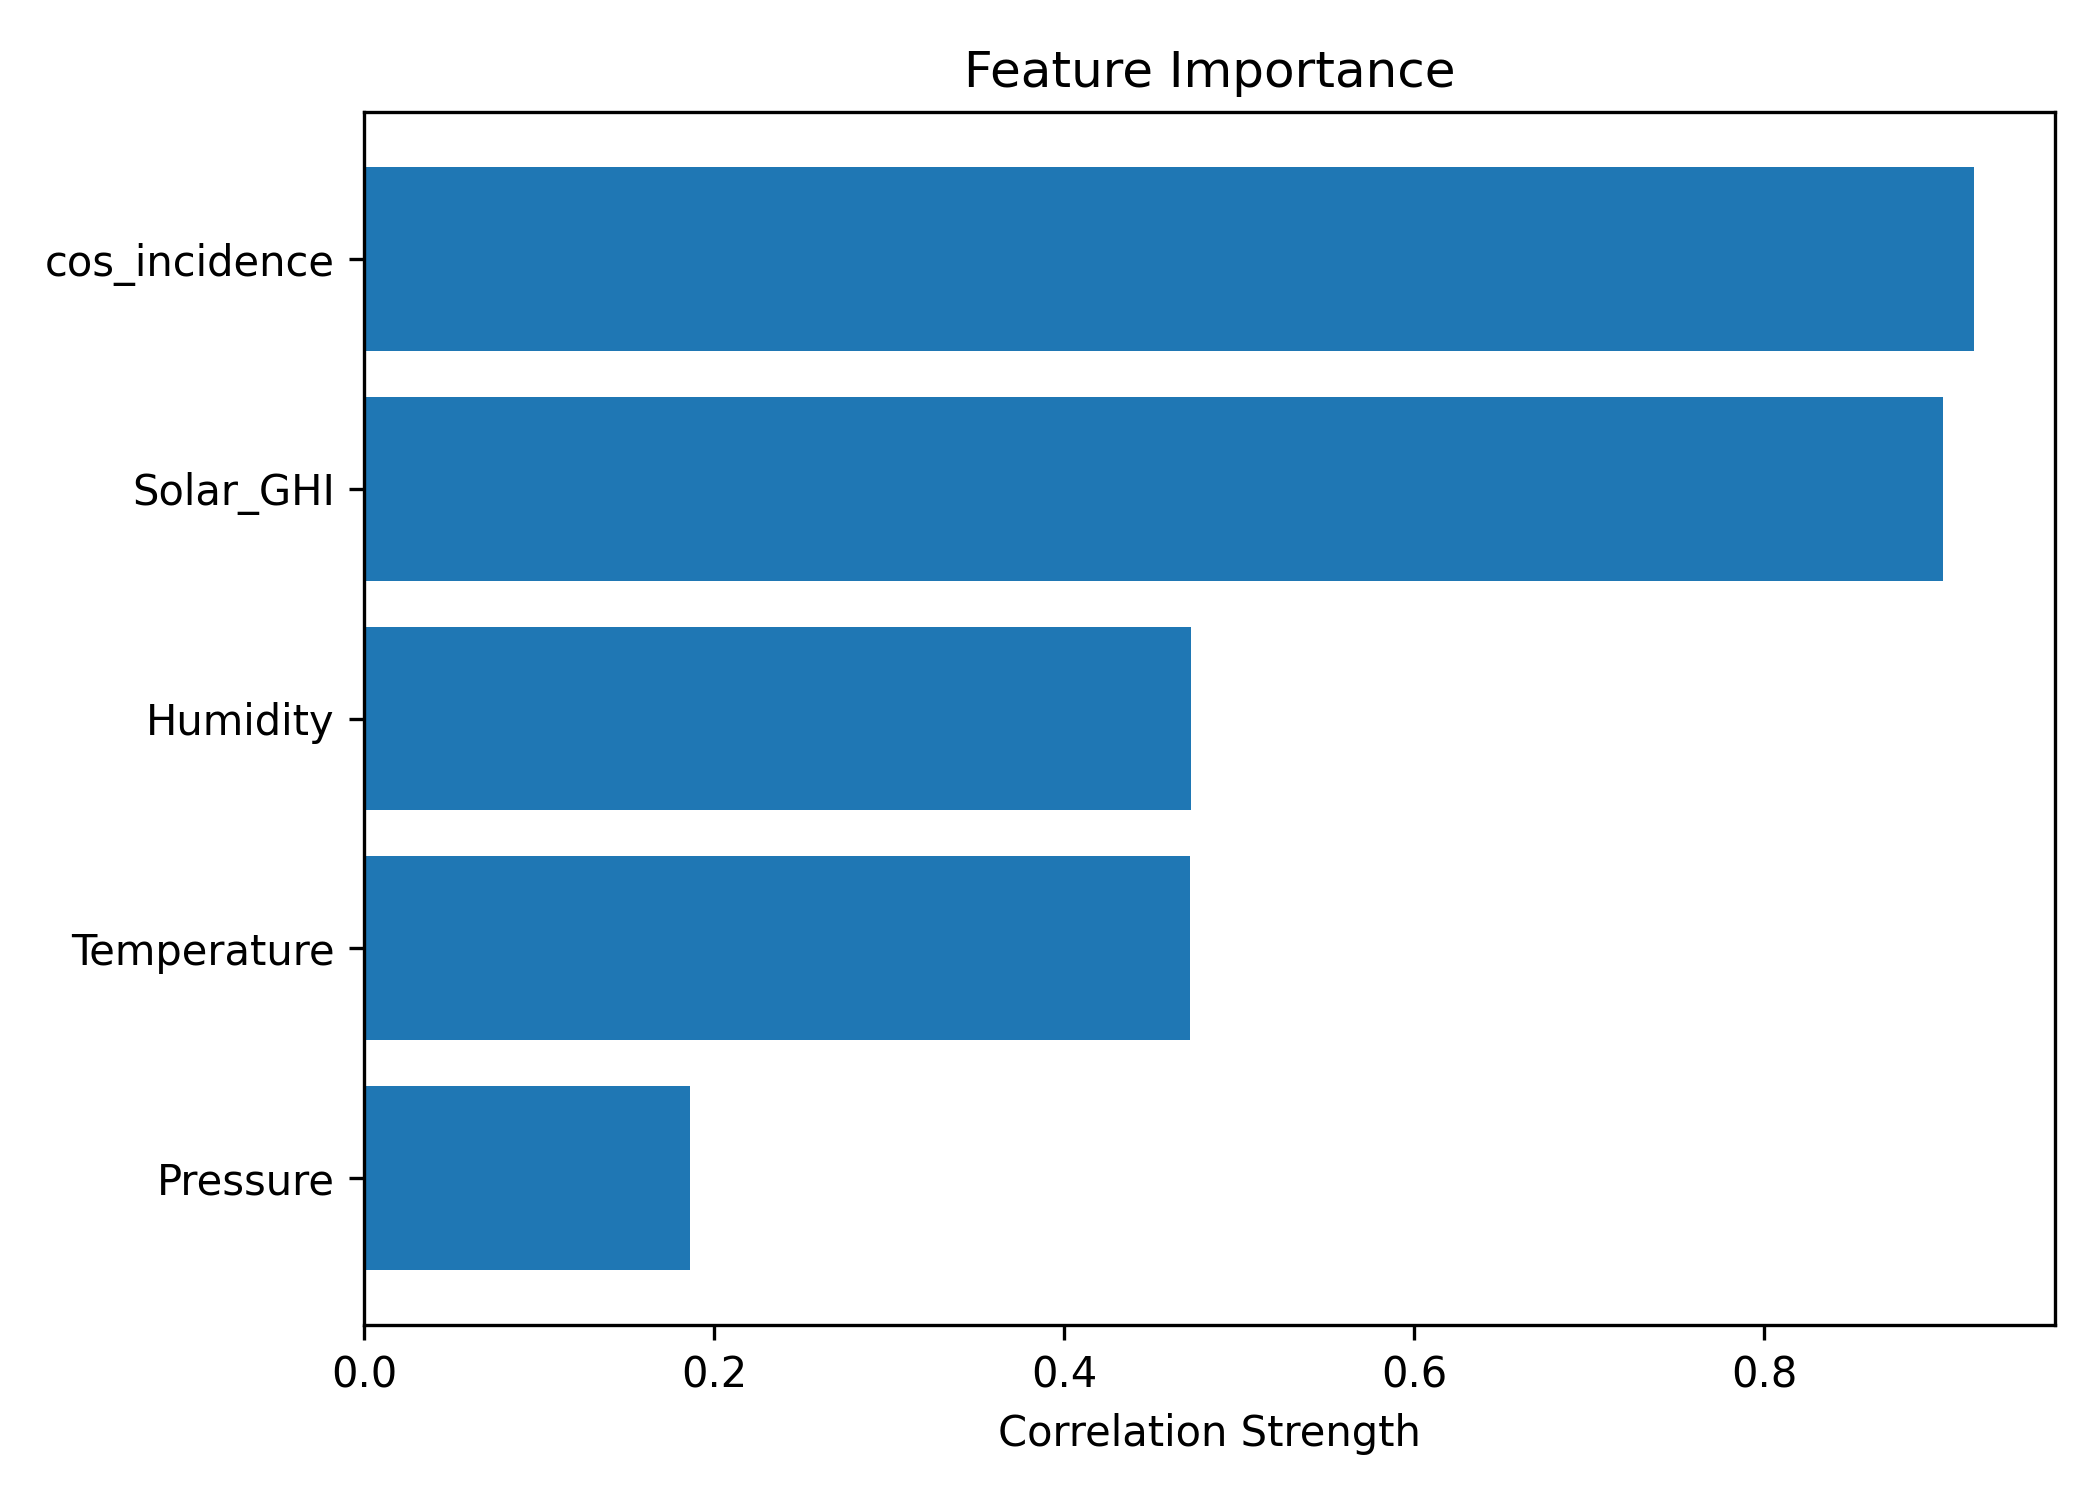
\includegraphics[width=0.7\textwidth]{picture/5_feature_importance.png}
    \caption[Feature Importance]{Feature Importance}
    \label{fig:image3}
\end{figure}

\vspace{10pt}
\begin{flushleft}
\hspace*{0.5cm}
จากรูปจะเห็นได้ว่าค่ามุมตกกระทบของแสงกับแผงโซลาร์เซลล์ (cos\_incidence) เป็นตัวแปรที่มีความสำคัญมากที่สุดรองลงมาก็คือ ความเข้มแสง (Solar\_GHI) ต่อมาคือความชื้นและอุณหภูมิ มีความสำคัญในระดับปานกลาง และสุดท้ายที่ส่งผลต่อโมเดลน้อยที่สุดคือ ความกดอากาศ
\end{flushleft}


\section{การทำงานของ Web Dashboard}

\subsection{หน้าแรก}

\begin{figure}[H]
    \centering
    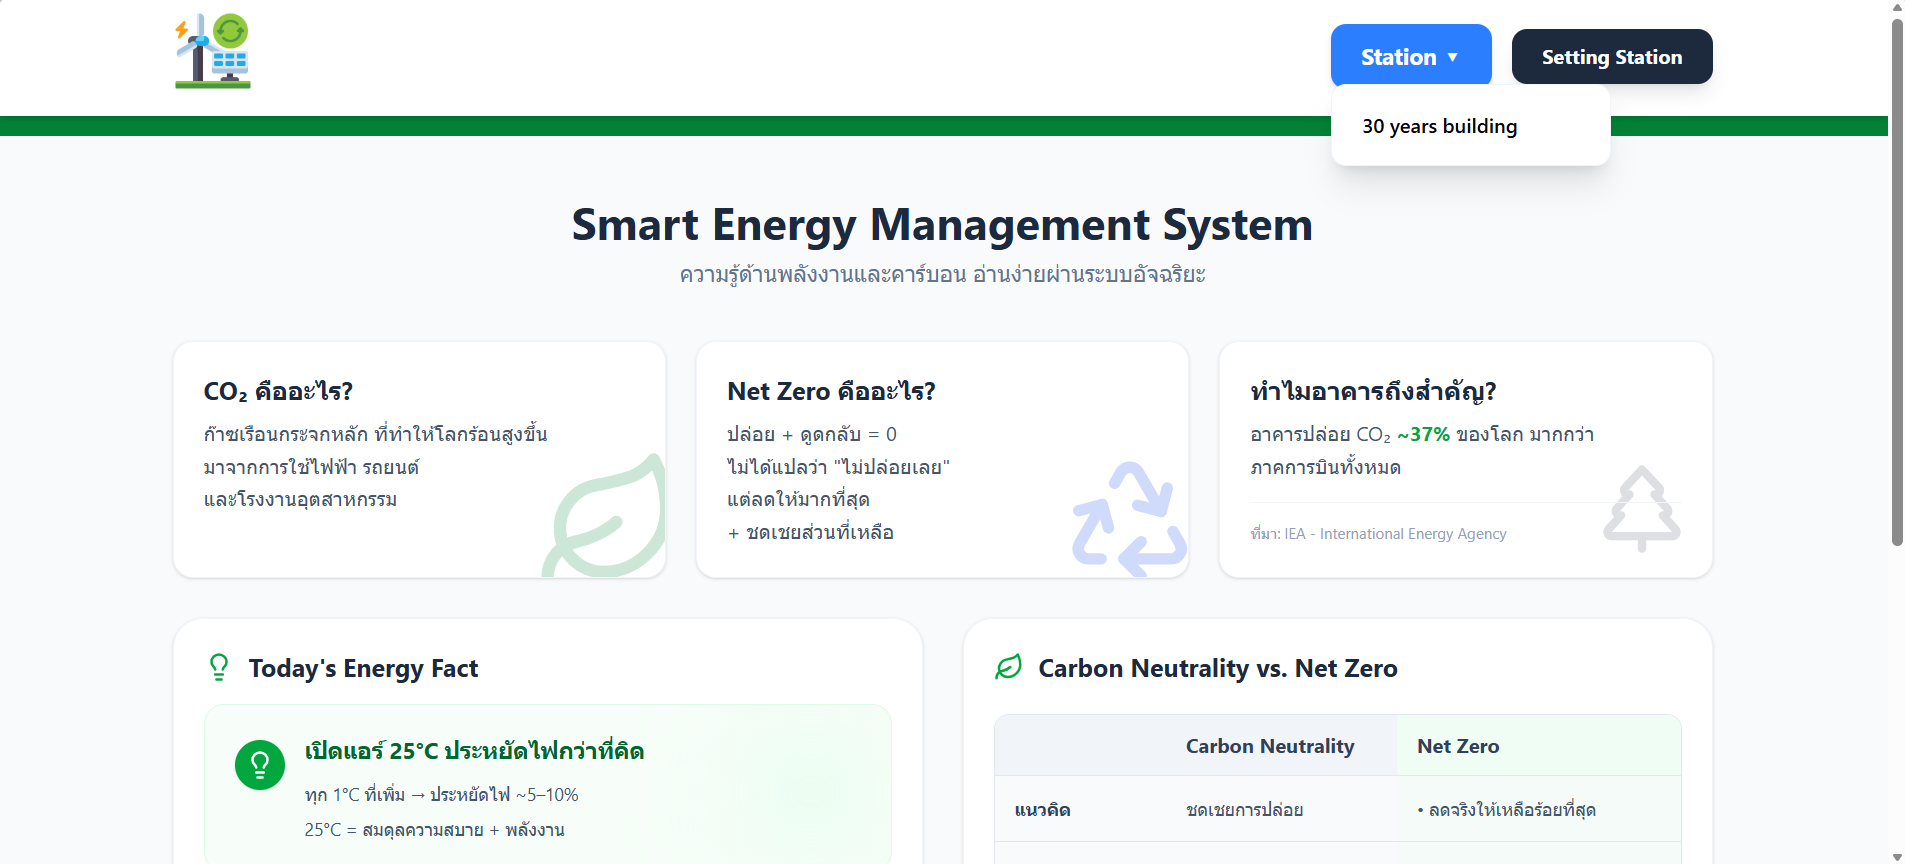
\includegraphics[width=0.7 \textwidth]{picture/Home.png}
    \caption[หน้าแรก]{หน้าแรก}
    \label{fig:image4}
\end{figure}

\vspace{10pt}
\begin{itemize}
    \item[]\textbf{4.3.1 ผลการประเมินเชิงตัวเลข} ค่าประสิทธิภาพของโมเดลมีดังนี้
    \begin{itemize}
        \item $R^2$ = 0.8619
        \item MAE = 2.427 kWh
    \end{itemize}

    \item[]\textbf{4.3.2 กราฟ Actual vs Predicted} 
    
    \hspace{\parindent} จากกราฟเปรียบเทียบค่า Actual และ Prediction โดยแกน x คือ Actual และ แกน y คือ Prediction โดยพบว่าค่าการทำนายมีความสอดคล้องกับค่าจริงในภาพรวม โดยจุดข้อมูลส่วนใหญ่กระจายตัวใกล้กับเส้นทแยงมุมสีแดง แสดงให้เห็นว่าโมเดลสามารถเรียนรู้ความสัมพันธ์ระหว่างตัวแปรสภาพอากาศกับการผลิตไฟฟ้าจากโซลาร์เซลล์ได้อย่างมีประสิทธิภาพ อย่างไรก็ตาม ในช่วงค่าการผลิตไฟฟ้าสูง จะพบการกระจายตัวของจุดข้อมูลเพิ่มขึ้น ซึ่งสะท้อนให้เห็นว่าความคลาดเคลื่อนของโมเดลมีแนวโน้มเพิ่มขึ้นเมื่อกำลังผลิตสูงขึ้น อาจเกิดจากความผันผวนของสภาพอากาศแบบฉับพลัน เช่น เมฆบังแดด หรือการเปลี่ยนแปลงของอุณหภูมิที่รวดเร็ว
    
    \begin{figure}[H]
    \centering
    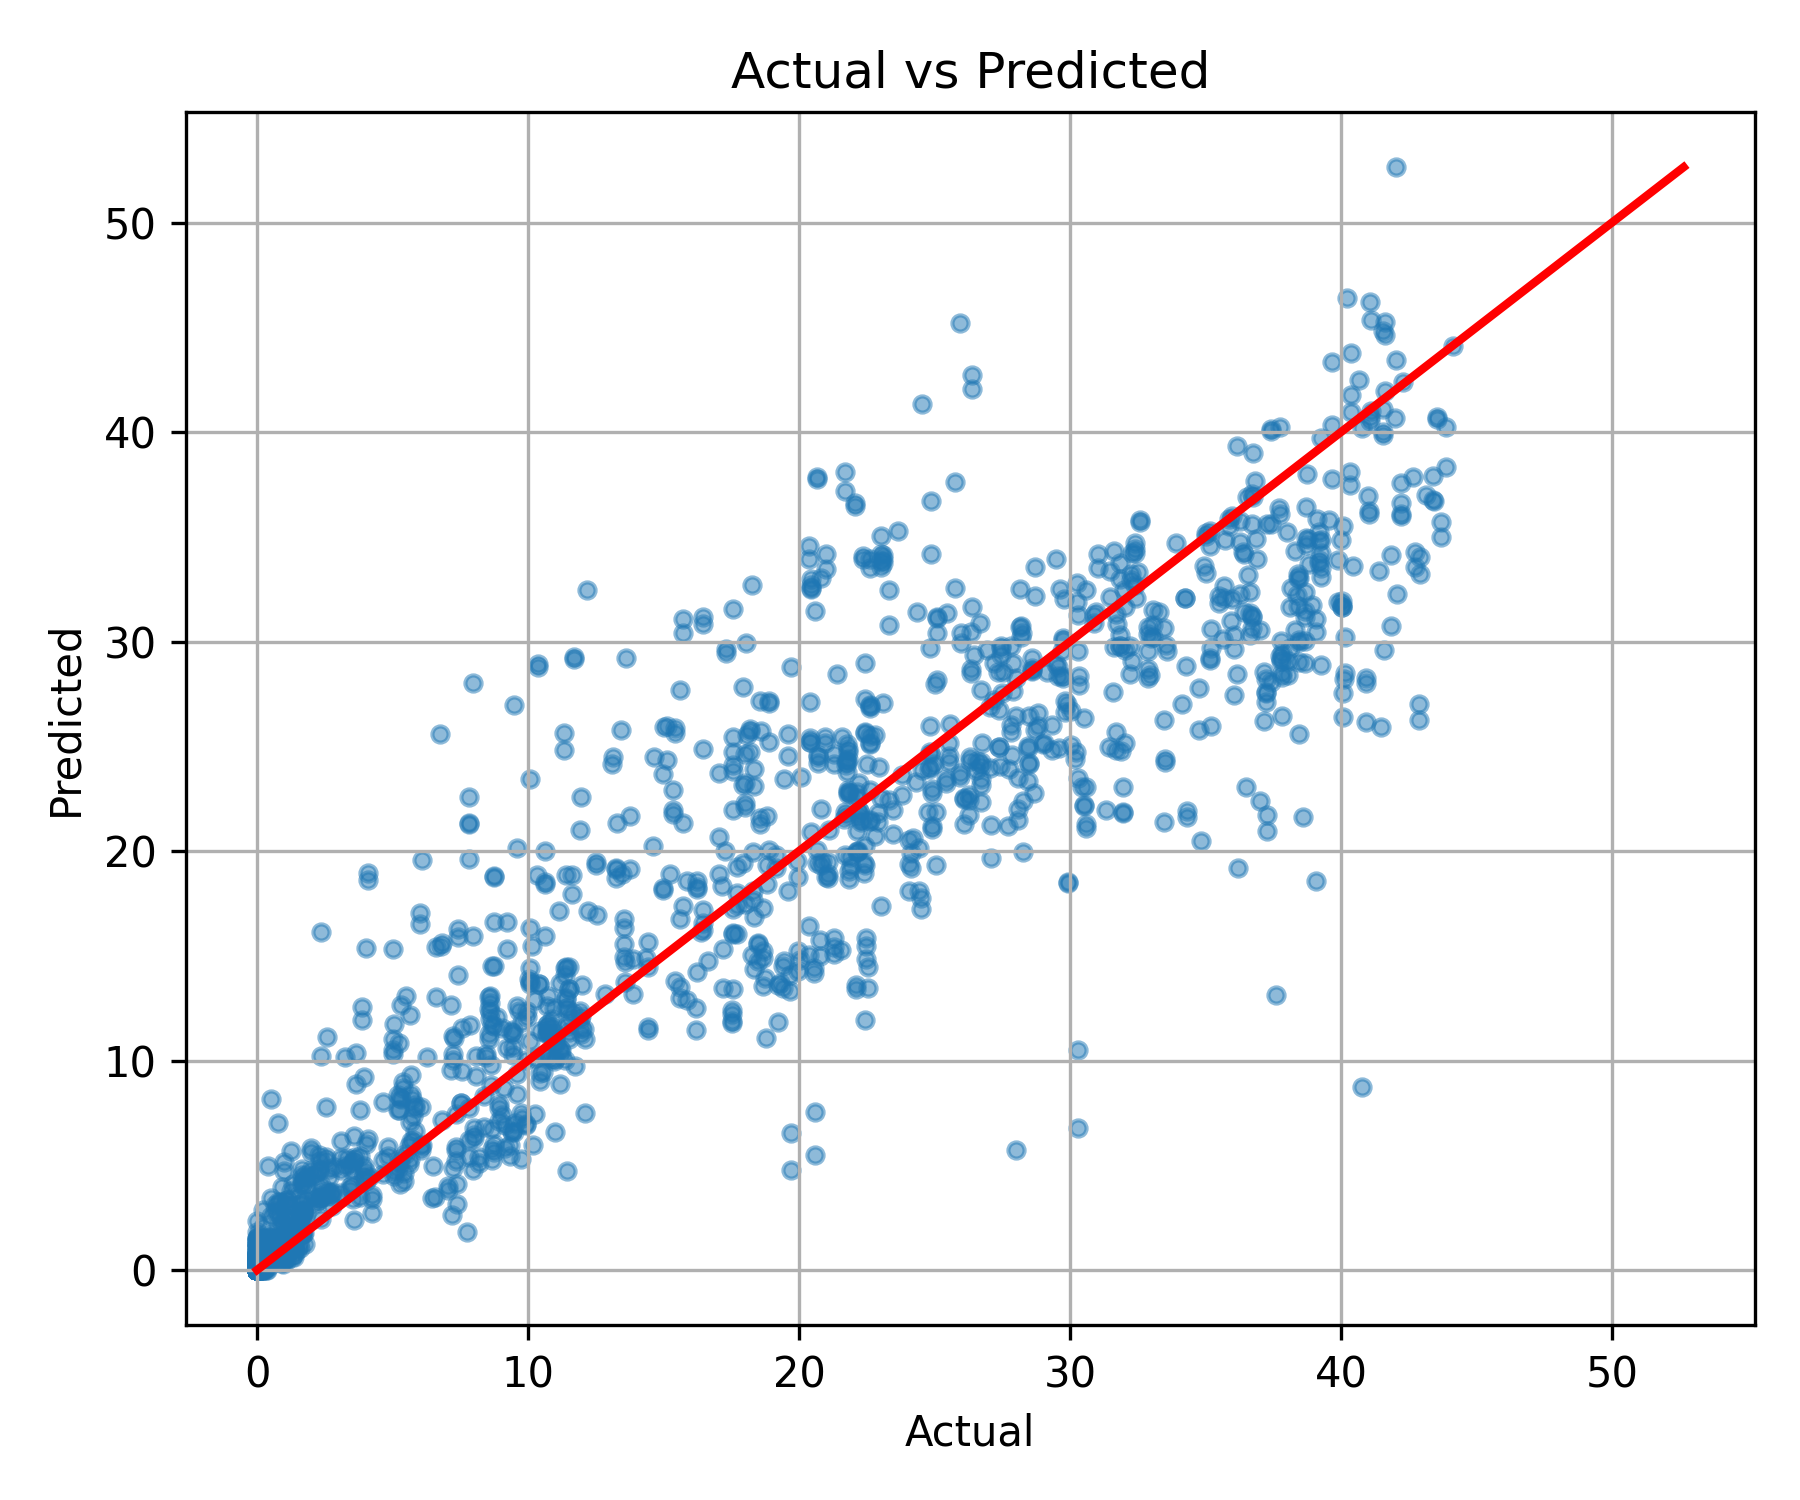
\includegraphics[width=0.7\textwidth]{picture/2_actual_vs_predicted.png}
    \caption[กราฟ Actual vs Predicted]{กราฟ Actual vs Predicted}
    \label{fig:Actual vs Predicted}
    \end{figure}
 
    \item[]\textbf{4.3.3 กราฟ Residual Plot} 
    
    \hspace{\parindent} จากกราฟจะพบว่าค่าความคลาดเคลื่อนส่วนใหญ่กระจายอยู่รอบค่า 0 แสดงว่าโมเดลไม่มีแนวโน้มทำนายค่าสูงเกินจริง หรือ ต่ำเกินจริง อย่างไรก็ตาม จะเห็นว่าการกระจายของ residual มีลักษณะขยายตัวมากขึ้นเมื่อค่าที่ทำนายมีค่าสูง ซึ่งแสดงถึงความแปรปรวนของความคลาดเคลื่อนที่เพิ่มขึ้นตามระดับกำลังผลิตไฟฟ้า 
    อาจเป็นผลมาจากปัจจัยภายนอกที่มีผลต่อการผลิตไฟฟ้าในช่วงเวลานั้น เช่น สภาพอากาศที่ไม่คงที่ หรือข้อจำกัดของชุดข้อมูลในการฝึกฝนโมเดล
   
    \begin{figure}[H]
    \centering
    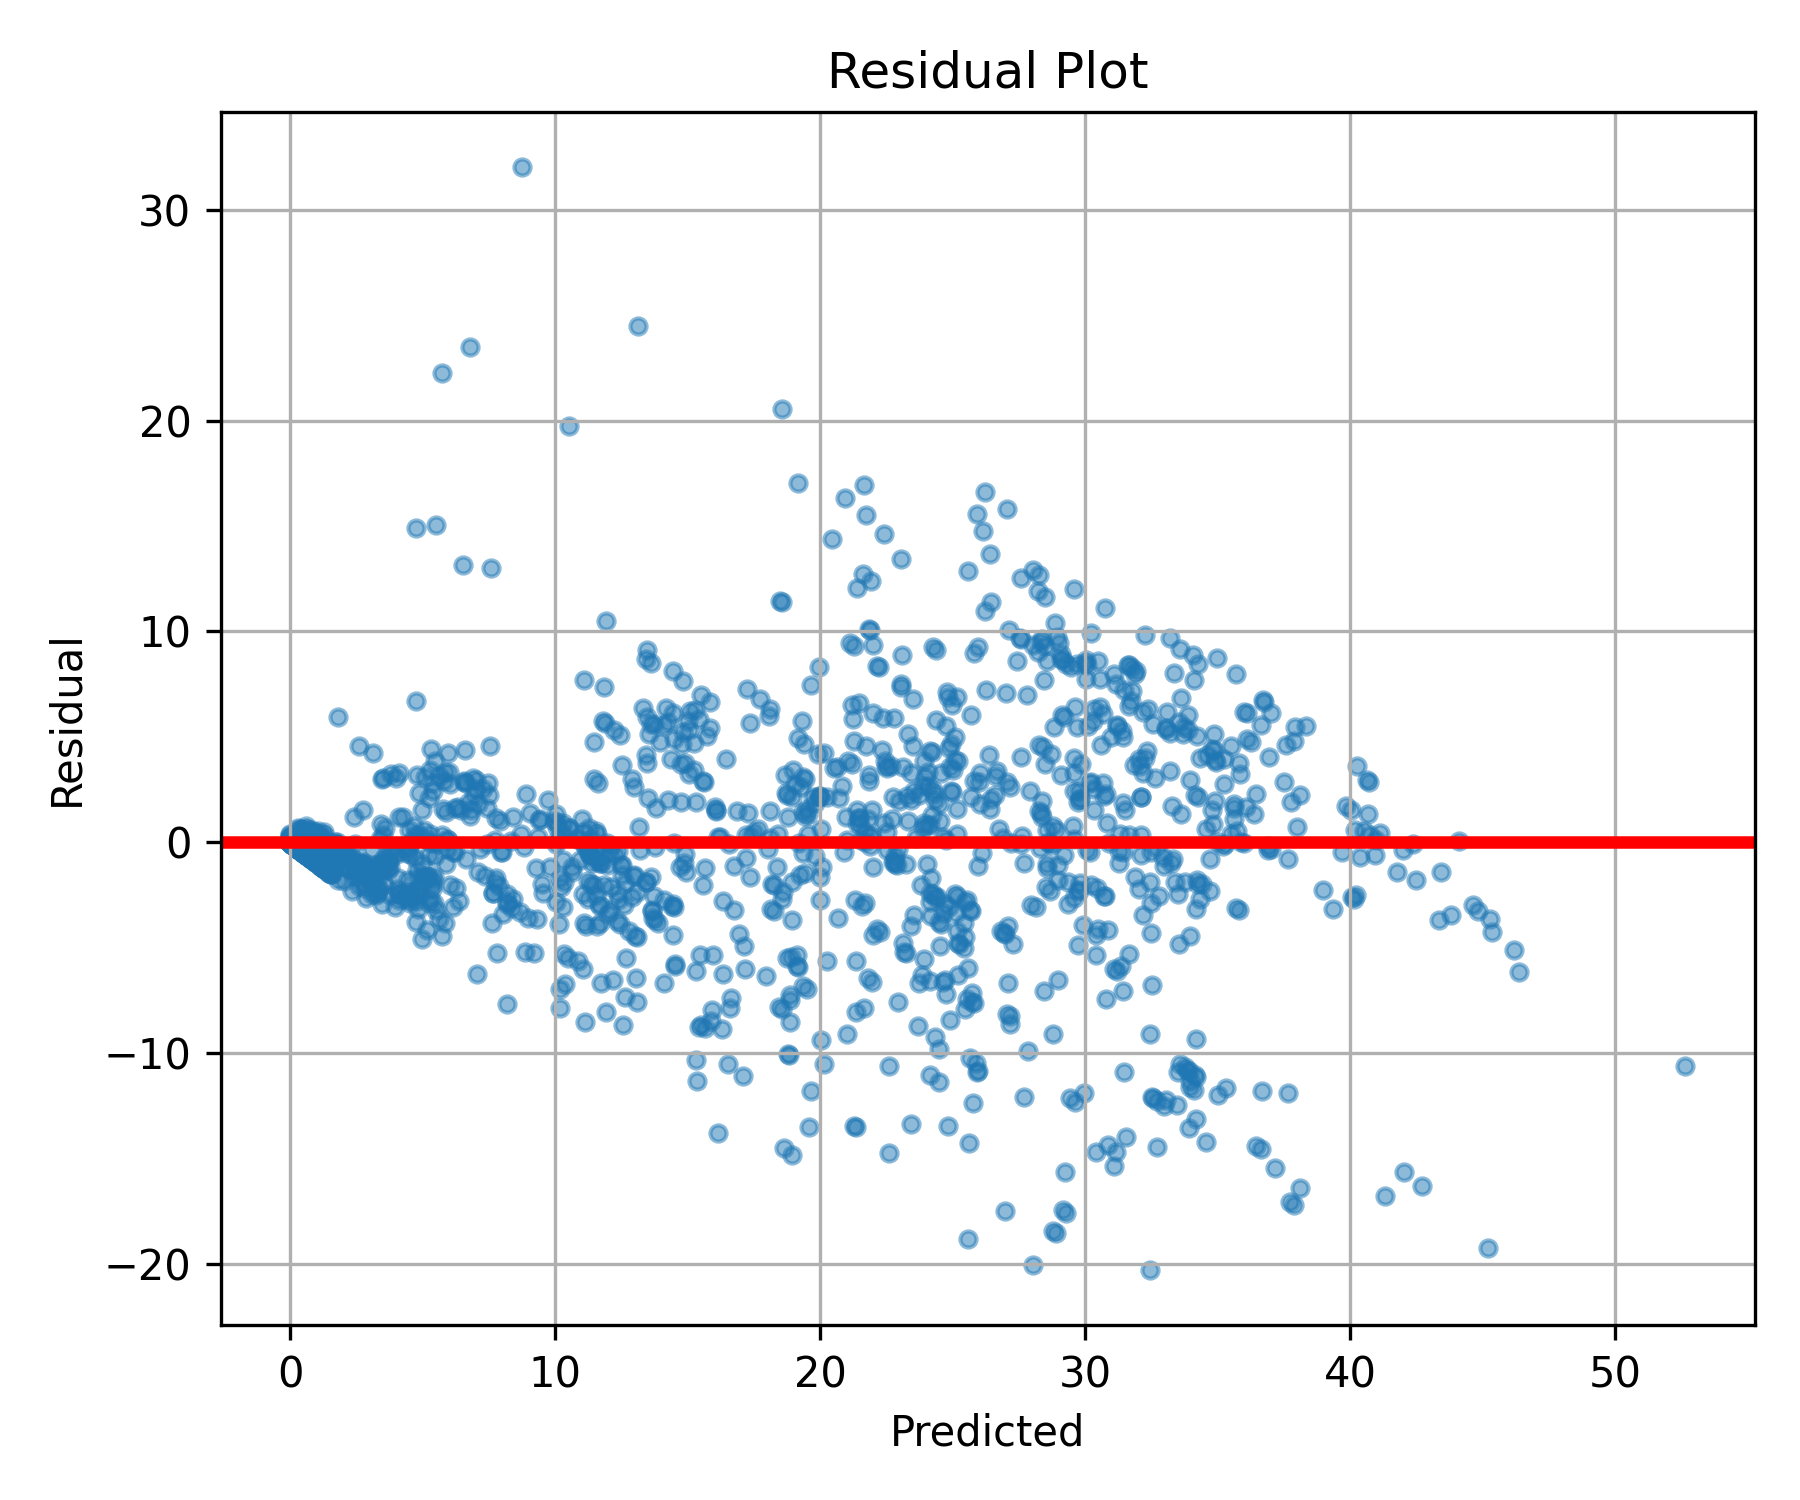
\includegraphics[width=0.7\textwidth]{picture/3_residual_plot.png}
    \caption[Residual Plot]{Residual Plot}
    \label{fig:Residual Plot}
    \end{figure}
   
    \item[] \textbf{4.3.4 กราฟ Feature Importance} 
    \hspace{\parindent} จากรูปจะเห็นได้ว่าค่ามุมตกกระทบของแสงกับแผงโซลาร์เซลล์ (cos\_incidence) เป็นตัวแปรที่มีความสำคัญมากที่สุดรองลงมาก็คือ ความเข้มแสง (Solar\_GHI) ต่อมาคือความชื้นและอุณหภูมิ มีความสำคัญในระดับปานกลาง และสุดท้ายที่ส่งผลต่อโมเดลน้อยที่สุดคือ ความกดอากาศ
    \begin{figure}[H]
    \centering
    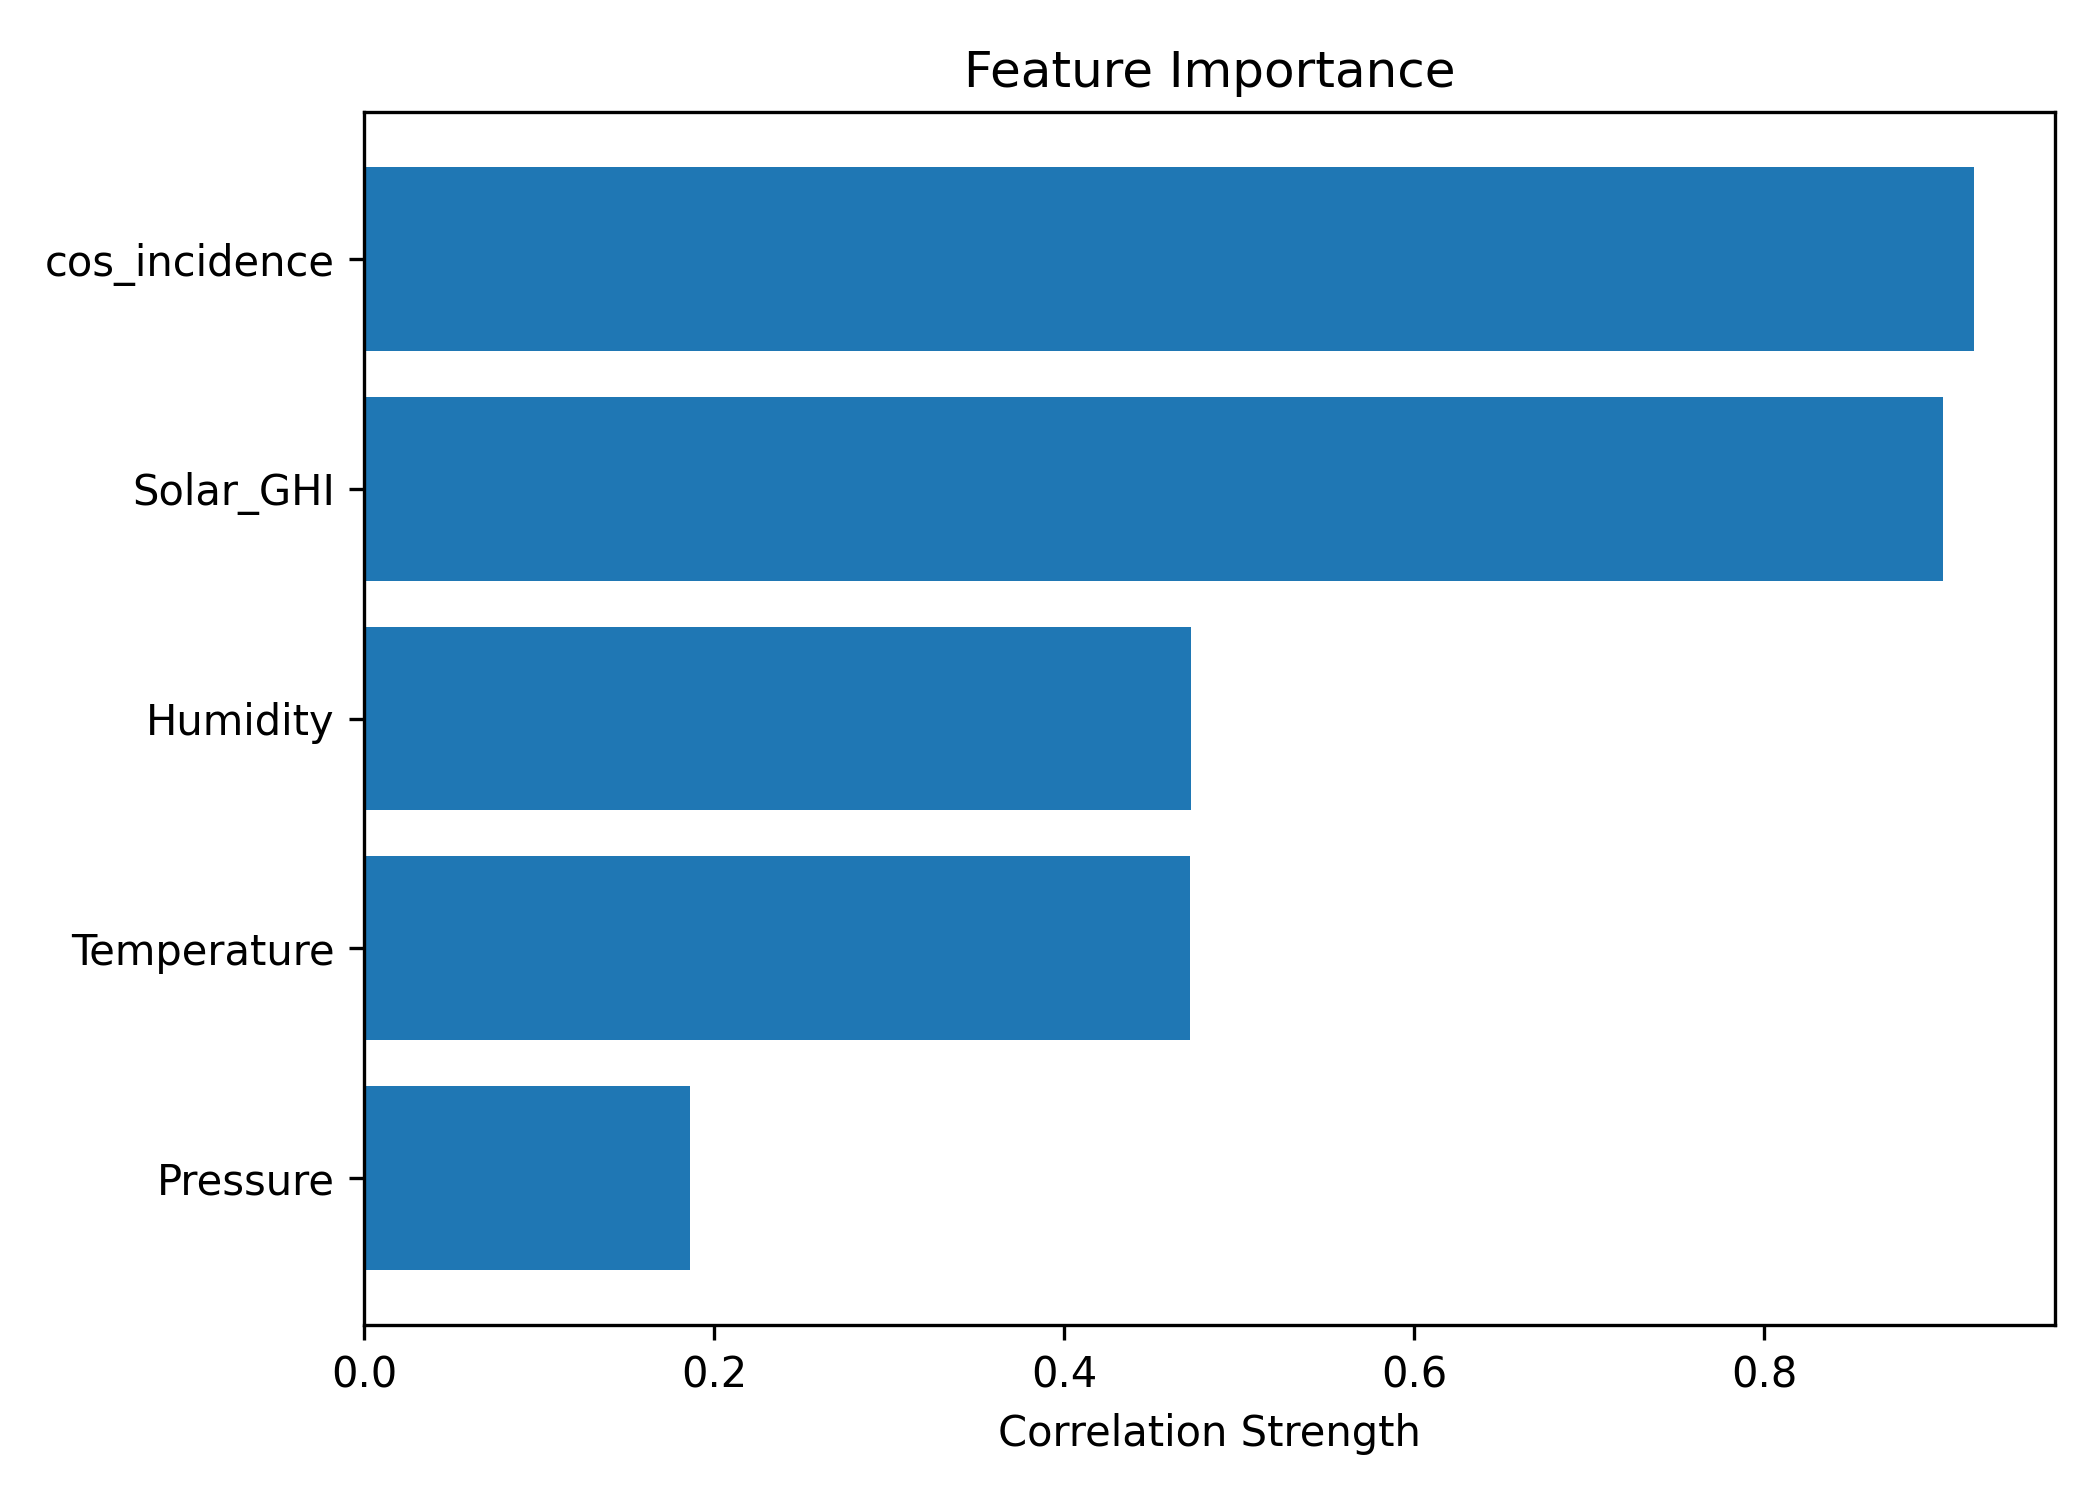
\includegraphics[width=0.7\textwidth]{picture/5_feature_importance.png}
    \caption[Feature Importance]{Feature Importance}
    \label{fig:Feature Importance}
    \end{figure}

\end{itemize}

\section{การใช้งานทั้งระบบ}
\begin{itemize}
    \item[]\textbf{4.4.1 การทดสอบการใช้งานระบบ} 
    \hspace{\parindent} ได้ทำการทดสอบการใช้งานระบบโดยการติดตั้งสถานีวัดสภาพอากาศขนาดย่อมที่บริเวณหลังคาของอาคาร ตึก 30 ปีคณะวิศวกรรมศาสตร์ มหาวิทยาลัยเชียงใหม่ และทำการทดสอบระบบโดยการให้ผู้ทดลองใช้งานระบบเพื่อดูข้อมูลสภาพอากาศและข้อมูลการพยากรณ์ปริมาณการผลิตไฟฟ้าจากโซลาร์เซลล์ล่วงหน้า 24 ชั่วโมง เป็นเวลา 10 วัน โดยผลการทดสอบพบว่ามีค่าความคลาดเคลื่อนเฉลี่ย 4.574 kWhต่อจุดข้อมูล ซึ่งเป็นผลมาจากความแปรปรวนของสภาพอากาศ และ ข้อจำกัดของชุดข้อมูลที่ใช้ในการฝึกฝนโมเดล เนื่องจากข้อมูลสภาพอากาศที่นำมาฝึกฝนโมเดลไม่ได้ใช้ค่าที่มาจากสถานีวัดสภาพอากาศที่ทำขึ้นแต่ตอนทดสอบใช้สภาพอากาศจากสถานีในการทำการทดสอบ จึงทำให้ค่าที่ทำนายการผลิตไฟฟ้านั้นเกิดความคลาดเคลื่อน 

    \begin{figure}[H]
    \centering
    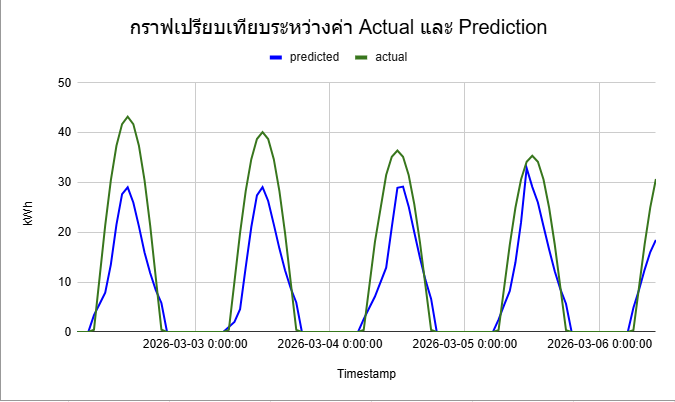
\includegraphics[width=0.7\textwidth]{picture/Test Station.png}
    \caption[การทดสอบการใช้งานระบบ]{การทดสอบการใช้งานระบบ}
    \label{fig:Test Station}
    \end{figure}

    \item[]\textbf{4.4.2 การประเมินความพึงพอใจในการใช้งานระบบ} 
    \hspace{\parindent} ได้ทําการประเมินความพึงพอใจในการใช้งานระบบ โดยมีนักศึกษามหาวิทยาลัยเชียงใหม่ 21 คนทําการประเมินโดยแบ่งเป็นผู้ชาย 10 คน และผู้หญิง 11 คน โดยให้คะแนนในแต่ละหัวข้อการประเมินตามความพึงพอใจในการใช้งานระบบ ซึ่งผลการประเมินมีดังนี้
    \begin{table}[H]
    \centering
    \renewcommand{\arraystretch}{1.5}
    \begin{tabular}{|l|c|}
    \hline 
    \multicolumn{1}{|c|}{\textbf{หัวข้อการประเมิน}} & \textbf{ความพึงพอใจ(เต็ม 5 คะแนน)} \\ \hline
    ด้านการออกแบบเว็บไซต์ (Interface Design) & 4.84 \\ \hline
    ด้านการแสดงผลข้อมูล (Data Visualization)   & 4.72 \\ \hline
    ด้านการใช้งานระบบ (Usability)   & 4.71 \\ \hline
    ด้านประสิทธิภาพของระบบ (System Performance)   & 4.67  \\ \hline
    ด้านประโยชน์ของระบบ (Usefulness) & 4.84  \\ \hline
    การเข้าถึงระบบ (Accessibility) & 4.80  \\ \hline
    \end{tabular}
    \caption{ประเมินความพึงพอใจในการใช้งานระบบ}
    \label{tab:satisfaction}
    \end{table}
    \vspace{10pt}
    \begin{flushleft}
    \hspace*{0.5cm}
    จากผลการประเมินความพึงพอใจรวมของผู้ทดลองใช้เว็บไซต์คือ 4.77 คะแนนหรือคิดเป็น 95.34\%
    \end{flushleft}
\end{itemize}


\section{วิเคราะห์และอภิปรายผล}
\hspace{\parindent} จากการใช้งานระบบพยากรณ์ปริมาณการผลิตไฟฟ้าจากแผงโซลาร์เซลล์ ซึ่งประกอบด้วยสถานีวัดสภาพอากาศขนาดย่อม Web Dashboard และ โมเดล Machine Learning สามารถวิเคราะห์และอภิปรายผลได้ดังนี้

\begin{figure}[H]
\centering
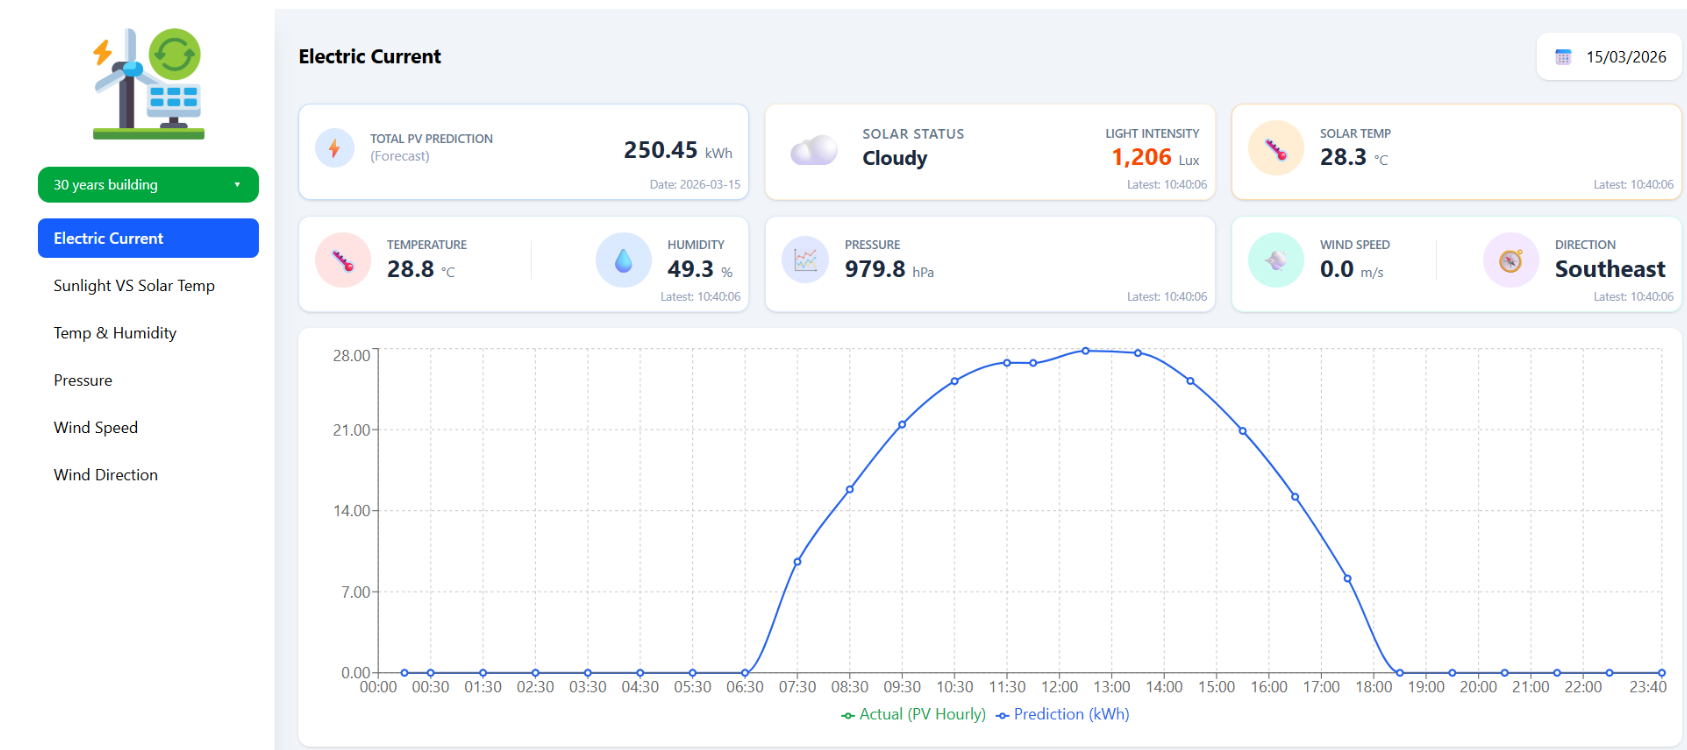
\includegraphics[width=0.7\textwidth]{picture/prediction.png}
\caption[หน้าแสดงข้อมูลการพยากรณ์ปริมาณการผลิตไฟฟ้าจากแผงโซลาร์เซลล์]{หน้าแสดงข้อมูลการพยากรณ์ปริมาณการผลิตไฟฟ้าจากแผงโซลาร์เซลล์}
\label{fig:image5}
\end{figure}

\vspace{10pt}
\begin{itemize}
    \item แสดงผลรวมการพยากร์ณปริมาณการผลิตไฟฟ้าจากโซลาร์เซลล์
    \item แสดงข้อมูลสภาพอากาศล่าสุดที่วัดได้จากเซ็นเซอร์
    \item แสดงกราฟการผลิตไฟฟ้าแบบรายชั่วโมงที่พยากรณ์ไว้ล่วงหน้า
\end{itemize}

\subsection{หน้าแสดงข้อมูลปริมาณไฟฟ้าที่ผลิตได้จริงจากแผงโซลลาร์เซลล์}

\begin{figure}[H]
\centering
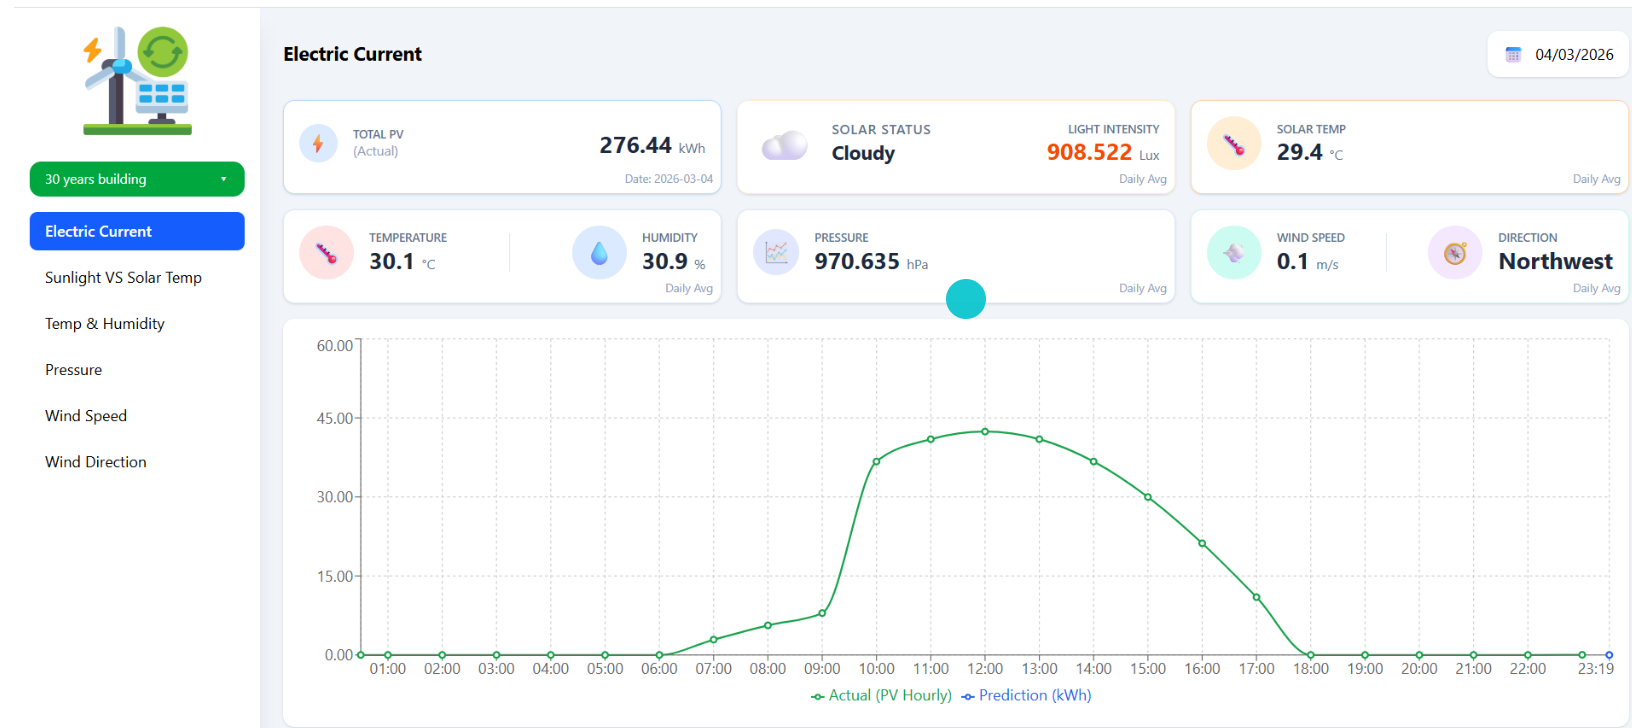
\includegraphics[width=0.7\textwidth]{picture/Electric Current.png}
\caption[หน้าแสดงข้อมูลปริมาณไฟฟ้าที่ผลิตได้จริงจากแผงโซลลาร์เซลล์]{หน้าแสดงข้อมูลปริมาณไฟฟ้าที่ผลิตได้จริงจากแผงโซลลาร์เซลล์}
\label{fig:image6}
\end{figure}
\vspace{10pt}

\begin{itemize}
    \item แสดงผลรวมปริมาณการผลิตไฟฟ้าจากโซลาร์เซลล์ที่ได้ในแต่ละวัน
    \item แสดงข้อมูลสภาพอากาศภาพเฉลี่ยรายวันที่วัดได้จากเซ็นเซอร์
    \item แสดงกราฟปริมาณการผลิตไฟฟ้าที่เกิดขึ้นจริงแบบรายชั่วโมง
    \item ผู้ใช้สามารถเลือกดูข้อมูลย้อนหลังหรือล่วงหน้าได้ผ่านปฏิทินที่มุมขวาบน 
    \item ผู้ใช้สามารถเลือกดูข้อมูลของแต่ละอาคารได้จากเมนูด้านซ้าย
\end{itemize}

\subsection{หน้าแสดงข้อมูลปริมาณแสงอาทิตย์และอุณหภูมิแผงโซลลาร์เซลล์}

\begin{figure}[H]
\centering
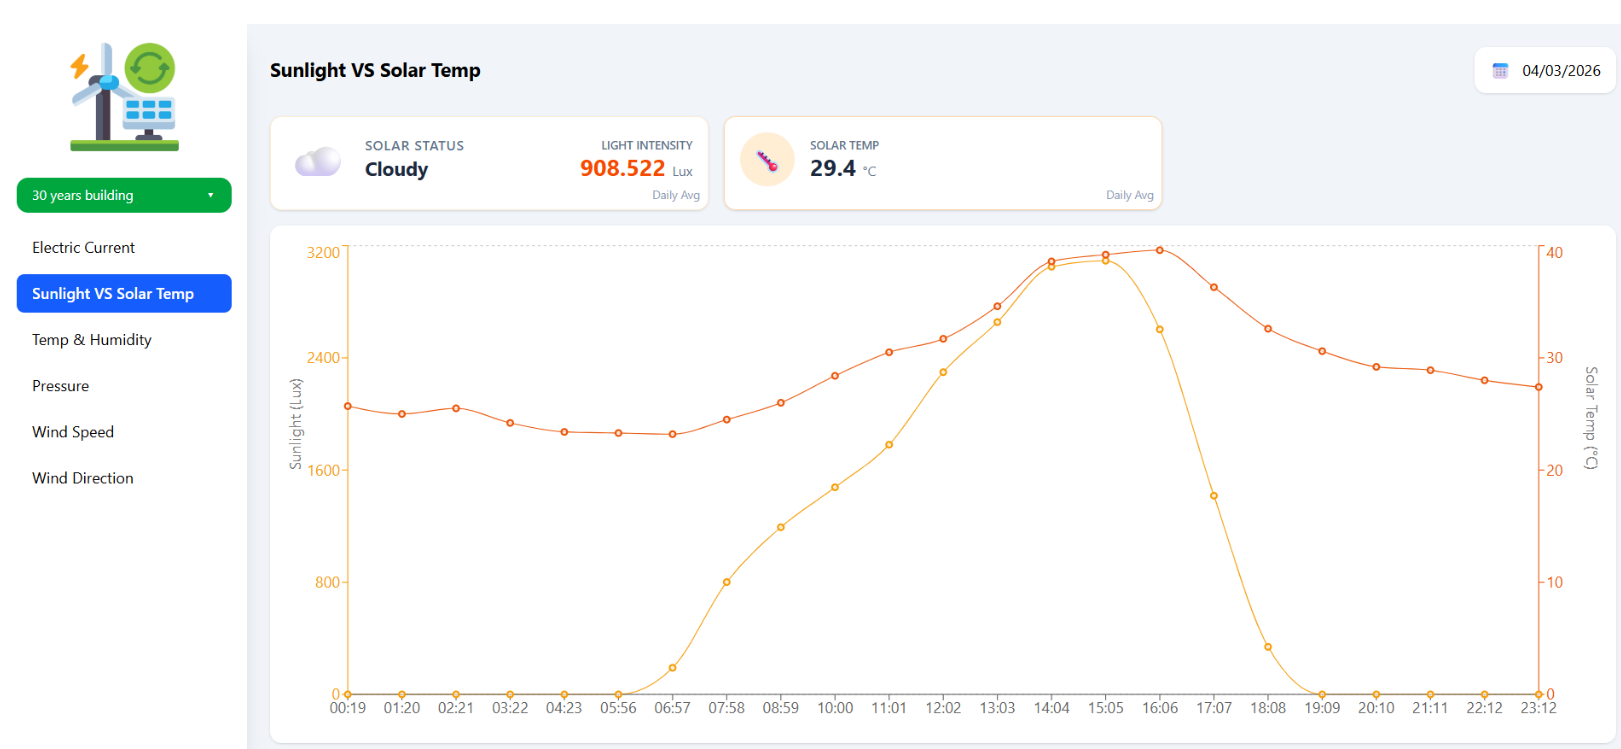
\includegraphics[width=0.7\textwidth]{picture/Sunlight VS Solar Temp.png}
\caption[หน้าแสดงข้อมูลปริมาณแสงอาทิตย์และอุณหภูมิแผงโซลลาร์เซลล์]{หน้าแสดงข้อมูลปริมาณแสงอาทิตย์และอุณหภูมิแผงโซลลาร์เซลล์}
\label{fig:image7}
\end{figure}

\vspace{10pt}
\begin{itemize}
    \item แสดงกราฟเปรียบเทียบระหว่างความเข้มแสงและอุณหภูมิแผงโซลลาร์เซลล์
    \item แสดงข้อมูลความเข้มแสงและอุณหภูมิแผงโซลลาร์เซลล์เฉลี่ยรายวัน 
    \item แสดงให้เห็นถึงความสัมพันธ์และแนวโน้มของอุณหภูมิแผงโซลาร์เซลล์ที่แปรผันตามความเข้มของแสงแดดในแต่ละช่วงเวลาของวัน
\end{itemize}

\subsection{หน้าแสดงข้อมูลอุณหภูมิและความชื้น}

\begin{figure}[H]
\centering
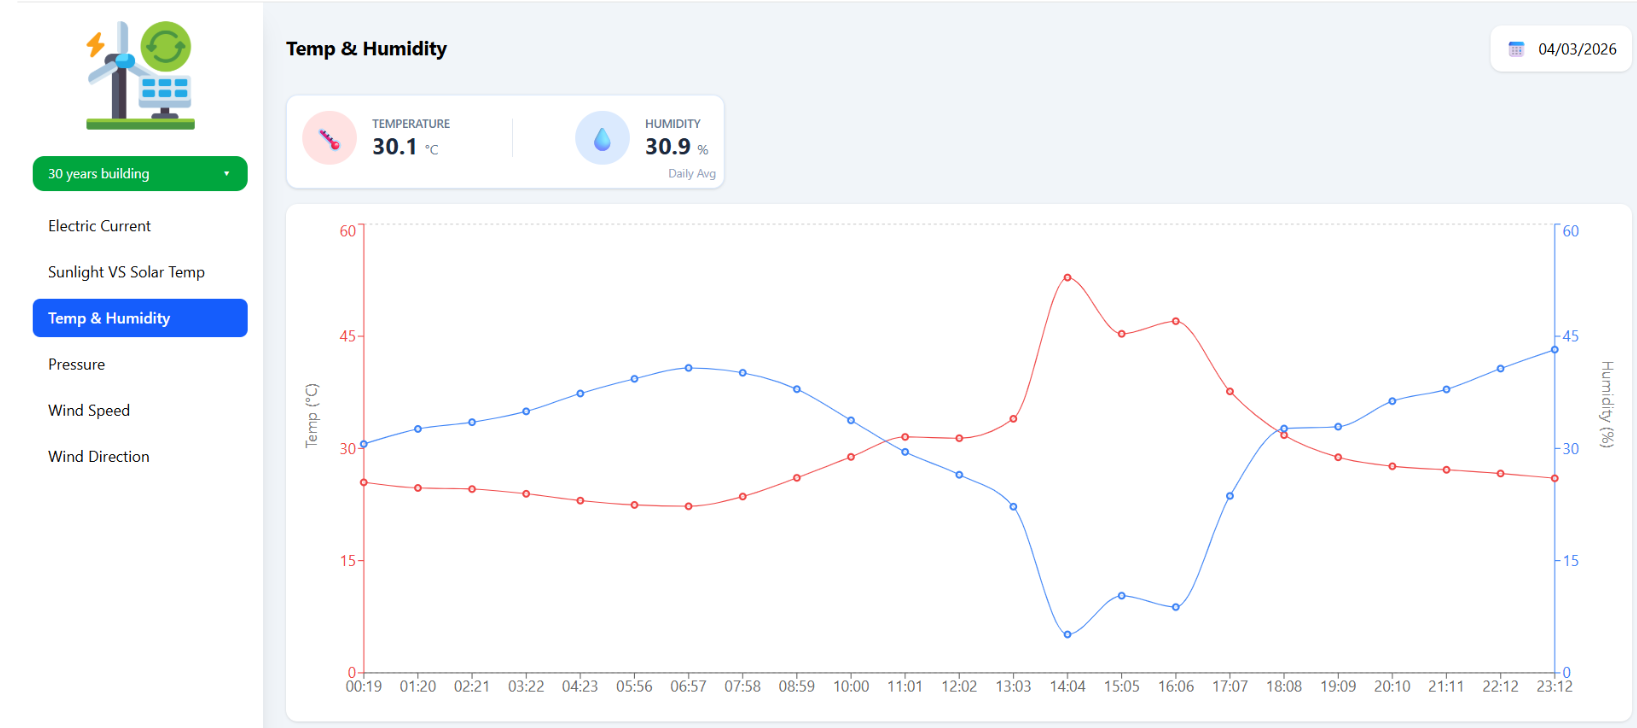
\includegraphics[width=0.7\textwidth]{picture/Temp and Humidity.png}
\caption[หน้าแสดงข้อมูลอุณหภูมิและความชื้น]{หน้าแสดงข้อมูลอุณหภูมิและความชื้น}
\label{fig:image8}
\end{figure}

\vspace{10pt}
\begin{itemize}
    \item แสดงกราฟเปรียบเทียบระหว่างอุณหภูมิและความชื้น
    \item แสดงข้อมูลอุณหภูมิและความชื้นเฉลี่ยรายวัน 
\end{itemize}



\subsection{หน้าแสดงข้อมูลความกดอากาศ}

\begin{figure}[H]
\centering
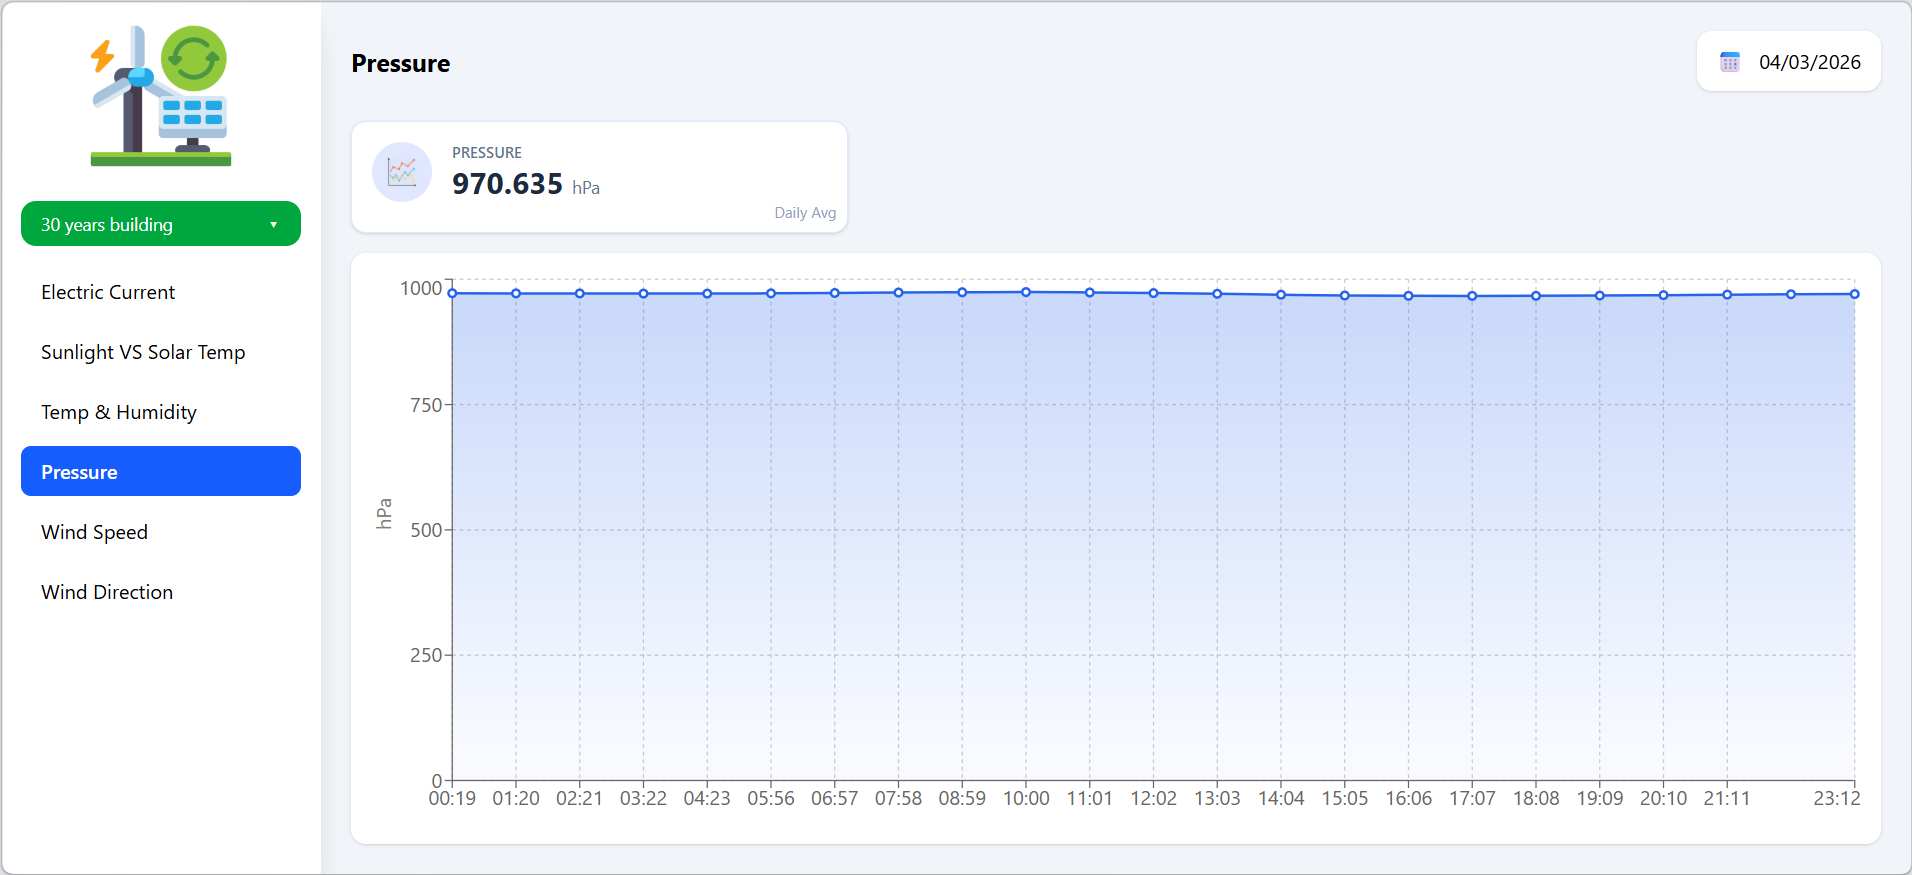
\includegraphics[width=0.7\textwidth]{picture/Pressure.png}
\caption[หน้าแสดงข้อมูลความกดอากาศ]{หน้าแสดงข้อมูลความกดอากาศ}
\label{fig:image9}
\end{figure}

\vspace{10pt}
\begin{itemize}
    \item แสดงข้อมูลความกดอากาศเฉลี่ยรายวัน 
    \item แสดงกราฟความกดอากาศในแต่ละช่วงเวลาของวัน เพื่อใช้เป็นข้อมูลประกอบในการวิเคราะห์การเกิดฝนตกหรือมีเมฆมาก
\end{itemize}

\subsection{หน้าแสดงข้อมูลความเร็วลม}

\begin{figure}[H]
\centering
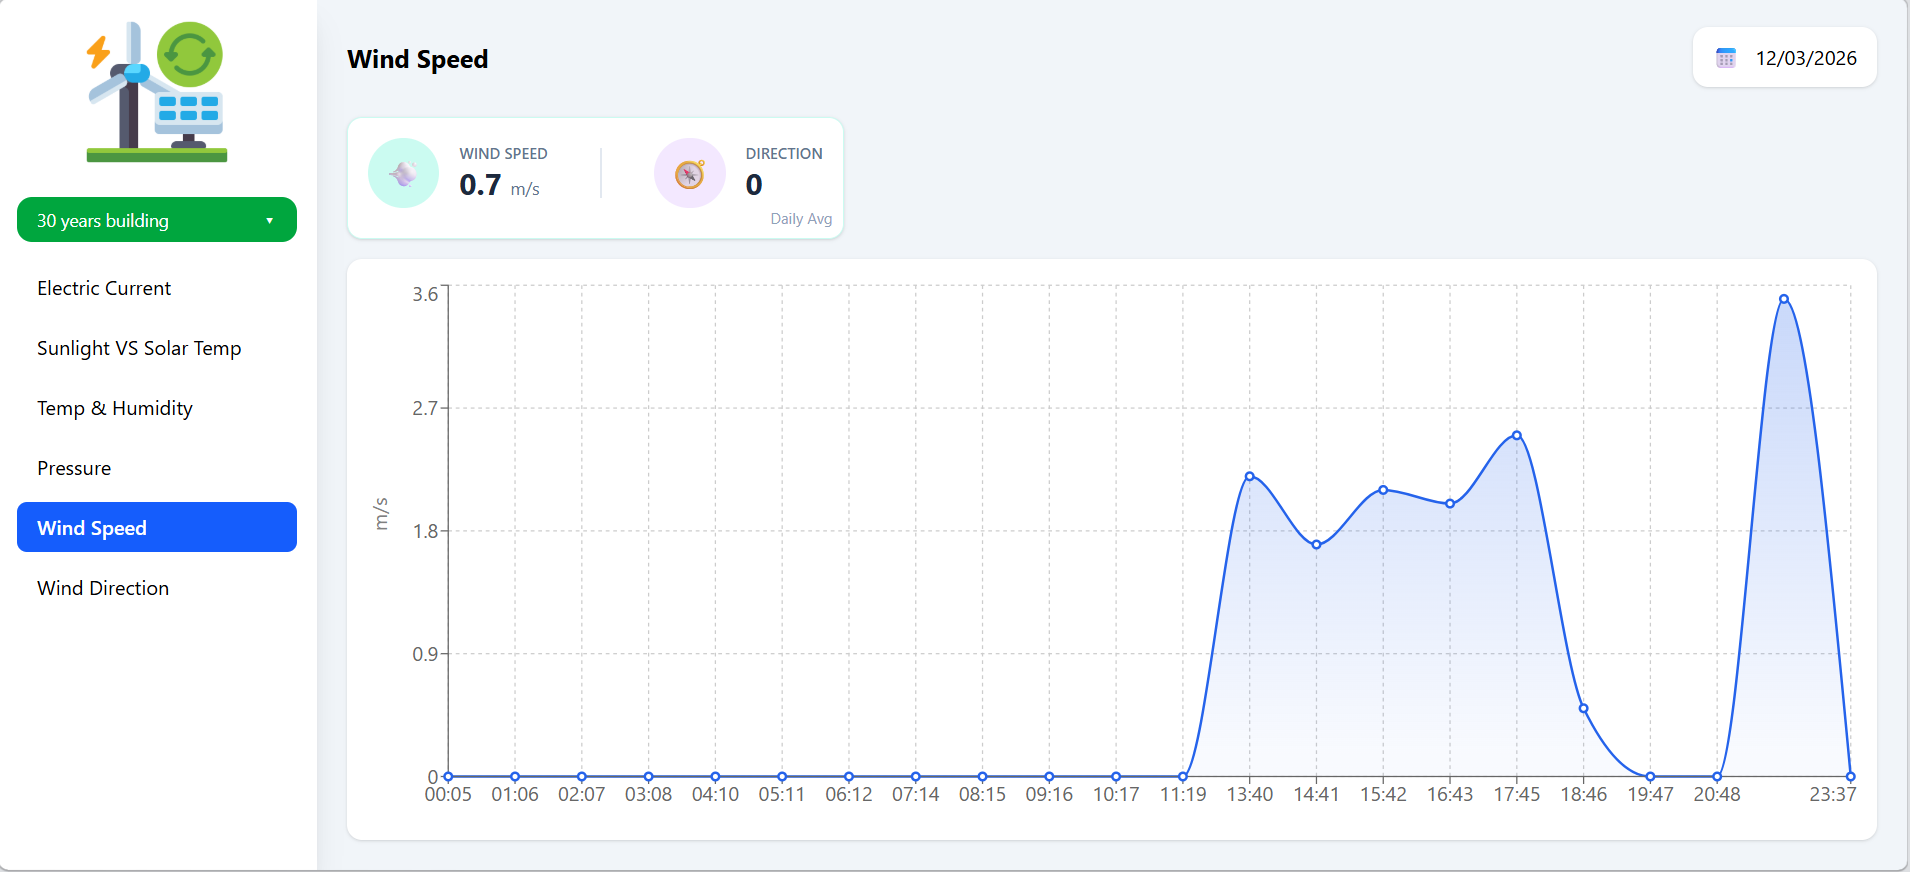
\includegraphics[width=0.7\textwidth]{picture/Wind Speed.png}
\caption[หน้าแสดงข้อมูลความเร็วลม]{หน้าแสดงข้อมูลความเร็วลม}
\label{fig:image10}
\end{figure}

\vspace{10pt}
\begin{itemize}
    \item แสดงข้อมูลความเร็วลมเฉลี่ยรายวัน 
    \item แสดงกราฟความเร็วลมในแต่ละช่วงเวลาของวัน เพื่อใช้เป็นข้อมูลประกอบในการวิเคราะห์ปัจจัยการระบายความร้อนของแผงโซลาร์เซลล์
\end{itemize}

\subsection{หน้าแสดงข้อมูลทิศทางลม}

\begin{figure}[H]
\centering
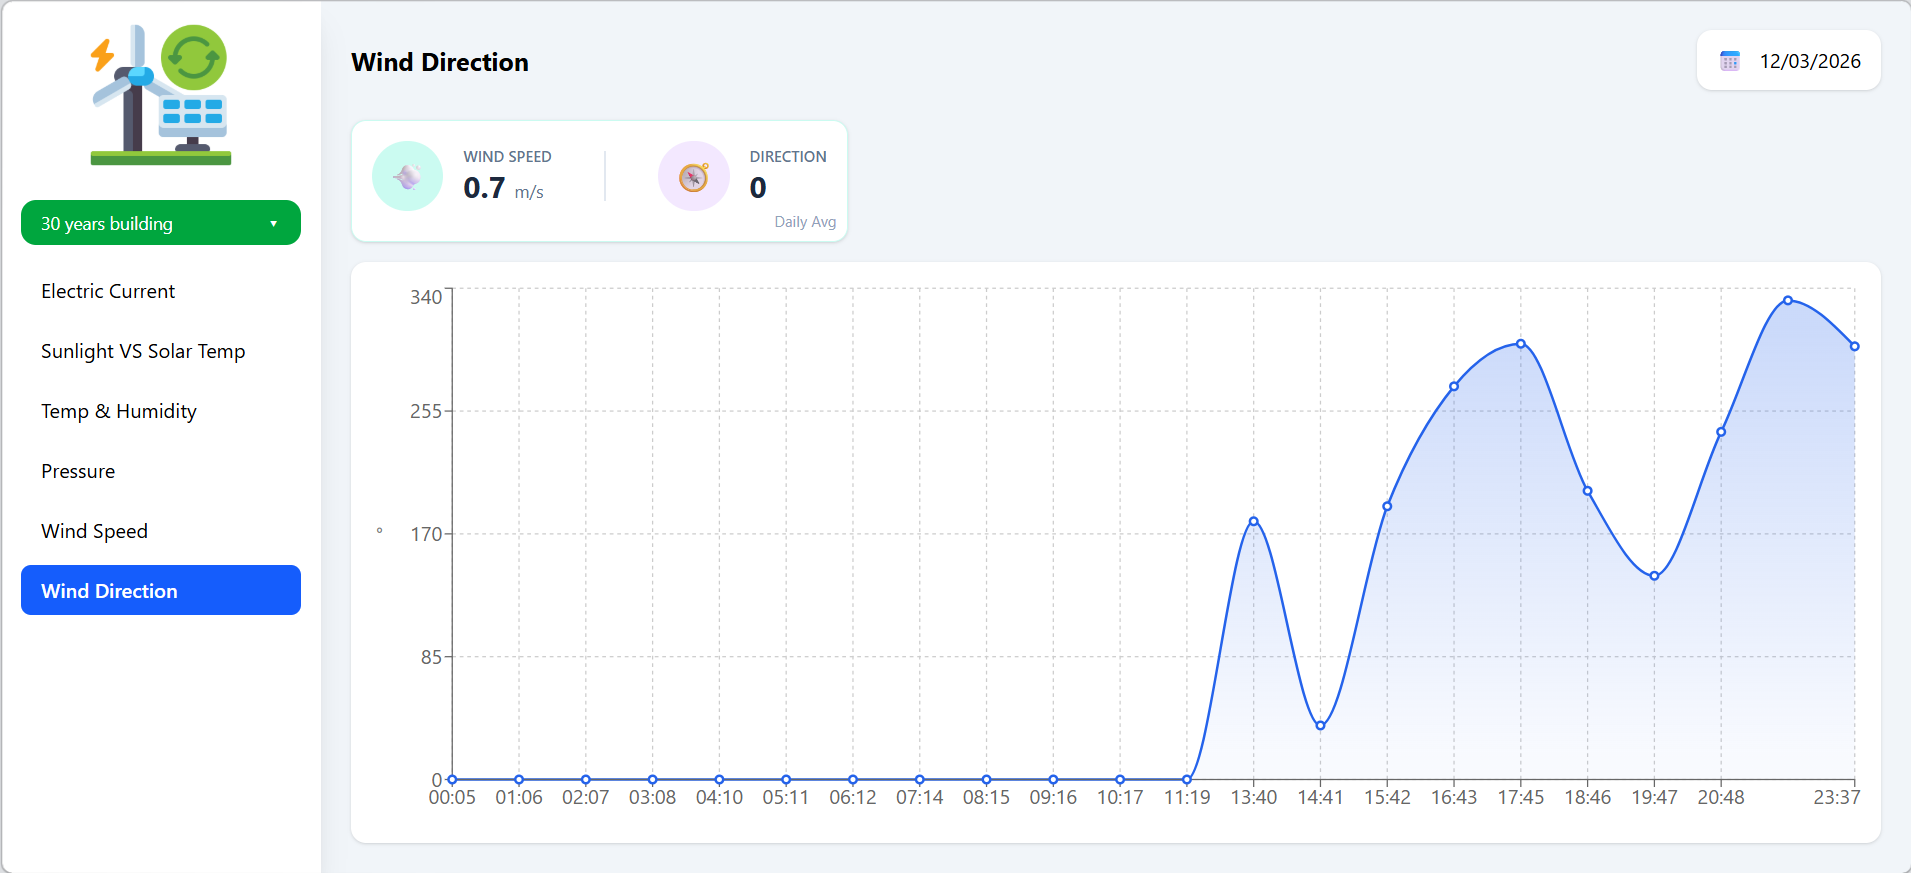
\includegraphics[width=0.7\textwidth]{picture/Wind Direction.png}
\caption[หน้าแสดงข้อมูลทิศทางลม]{หน้าแสดงข้อมูลทิศทางลม}
\label{fig:imag11}
\end{figure}

\begin{itemize}
    \item แสดงข้อมูลทิศทางลมเฉลี่ยรายวัน 
    \item แสดงกราฟการเปลี่ยนแปลงทิศทางลมในหน่วยองศาในแต่ละช่วงเวลาของวัน
\end{itemize}

\subsection{หน้าแสดงสถานะการทำงานของเซ็นเซอร์}

\begin{figure}[H]
\centering
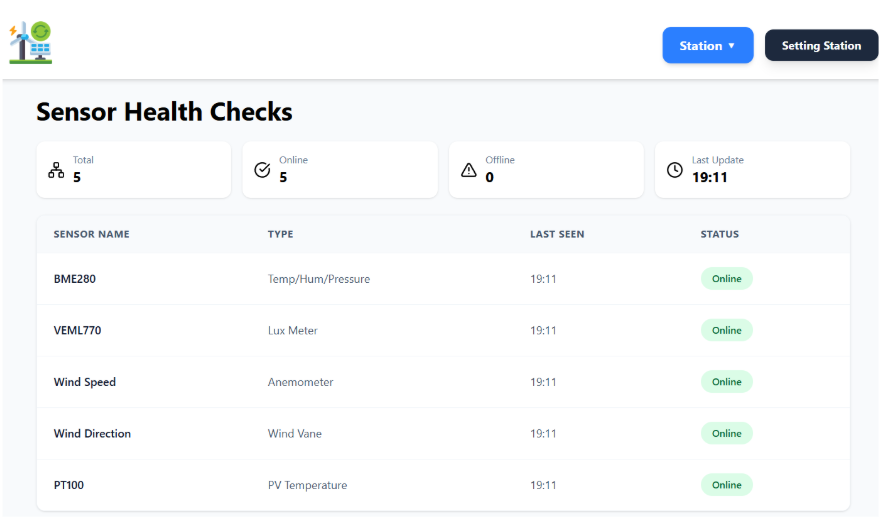
\includegraphics[width=0.7\textwidth]{picture/sensor check.png}
\caption[หน้าแสดงสถานะการทำงานของเซ็นเซอร์]{หน้าแสดงสถานะการทำงานของเซ็นเซอร์}
\label{fig:image12}
\end{figure}

\vspace{10pt}
\begin{itemize}
    \item แสดงข้อมูลภาพรวมต่างๆ ได้แก่ จำนวนเซ็นเซอร์ทั้งหมด จำนวนเซ็นเซอร์ที่ทำงานได้ปกติ จำนวนเซ็นเซอร์ที่ขาดการเชื่อมต่อ และเวลาที่ระบบได้รับการอัปเดตข้อมูลล่าสุด 
    \item แสดงรายละเอียดของอุปกรณ์แต่ละตัว ได้แก่ ชื่อเซ็นเซอร์ ประเภทการตรวจวัด เวลาที่ส่งข้อมูลเข้าเซิร์ฟเวอร์ครั้งล่าสุด และ สถานะการทำงาน 
    \item แสดงกราฟปริมาณการผลิตไฟฟ้าที่เกิดขึ้นจริงแบบรายชั่วโมง
    \item ผู้ใช้สามารถตรวจสอบสถานะการทำงานของเซ็นเซอร์ภายในสถานีวัดสภาพอากาศขนาดย่อมได้อย่างรวดเร็ว ซึ่งช่วยให้ง่ายต่อการซ่อมบำรุงเมื่ออุปกรณ์ตัวใดตัวหนึ่งเกิดปัญหา
\end{itemize}

\section{การประเมินความพึงพอใจในการใช้งานระบบ}

\hspace*{0.5cm}
ได้ทําการประเมินความพึงพอใจในการใช้งานระบบ โดยมีนักศึกษามหาวิทยาลัยเชียงใหม่ 21 คนทําการประเมินโดยแบ่งเป็นผู้ชาย 10 คน และผู้หญิง 11 คน โดยให้คะแนนในแต่ละหัวข้อการประเมินตามความพึงพอใจในการใช้งานระบบ ซึ่งผลการประเมินมีดังนี้
\begin{table}[H]
\centering
\renewcommand{\arraystretch}{1.5}
\begin{tabular}{|l|c|}
\hline
\textbf{หัวข้อการประเมิน} & \textbf{ความพึงพอใจ(เต็ม 5 คะแนน)} \\ \hline
ด้านการออกแบบเว็บไซต์ (Interface Design) & 4.84 \\ \hline
ด้านการแสดงผลข้อมูล (Data Visualization)   & 4.72 \\ \hline
ด้านการใช้งานระบบ (Usability)   & 4.71 \\ \hline
ด้านประสิทธิภาพของระบบ (System Performance)   & 4.67  \\ \hline
ด้านประโยชน์ของระบบ (Usefulness) & 4.84  \\ \hline
การเข้าถึงระบบ (Accessibility) & 4.80  \\ \hline
\end{tabular}
\caption{ตารางสรุปการประเมินความพึงพอใจในการใช้งานระบบ}
\label{tab:satisfaction}
\end{table}
\vspace{10pt}
\begin{flushleft}
\hspace*{0.5cm}
จากผลการประเมินความพึงพอใจรวมของผู้ทดลองใช้เว็บไซต์คือ 4.77 คะแนนหรือคิดเป็น 95.34\%
\end{flushleft}

Web Dashboard ที่พัฒนาขึ้นสามารถแสดงข้อมูลได้ถูกต้อง ผู้ใช้สามารถตรวจสอบข้อมูลสภาพอากาศ กราฟความสัมพันธ์ และผลการพยากรณ์ไฟฟ้าล่วงหน้าได้อย่างสะดวก โดยผลการประเมินความพึงพอใจเฉลี่ยอยู่ที่ 4.77 คะแนน หรือคิดเป็น 95.34\% สะท้อนให้เห็นว่าระบบช่วยให้ผู้ใช้งานเข้าถึงข้อมูลได้ง่าย และมีประโยชน์ต่อการวางแผนการใช้งานพลังงาน

โมเดลพยากรณ์ ผลการประเมินเชิงตัวเลขให้ค่า $R^2$ = 0.8619 และ MAE = 2.427 kWh แสดงว่าโมเดลมีประสิทธิภาพที่ดีสำหรับข้อมูลทดสอบที่เตรียมไว้ อย่างไรก็ตาม เมื่อนำไปใช้งานกับข้อมูลจริงพบว่าความคลาดเคลื่อนเฉลี่ยประมาณ 4.574 kWh เนื่องจากข้อมูลฝึกไม่ได้ใช้ข้อมูลที่ได้มาจากสถานีวัดสภาพอากาศที่ตั้งขึ้น รวมถึงปัจจัยแสงแดดและสภาพอากาศที่แปรผันแบบฉับพลันที่โมเดลอาจจะยังไม่สามารถเรียนรู้ได้ นอกจากนี้กราฟ Actual vs Predicted และ Residual Plot ยังแสดงให้เห็นว่าโมเดลมีความแม่นยำมากในช่วงกำลังผลิตระดับปานกลาง แต่มีความคลาดเคลื่อนเพิ่มขึ้นในช่วงกำลังผลิตสูง ซึ่งเป็นช่วงที่สภาพแสงไม่คงที่มากที่สุด

โดยสรุป ระบบทั้งหมดสามารถทำงานร่วมกันได้อย่างสมบูรณ์ ตั้งแต่การเก็บข้อมูล การประมวลผล การพยากรณ์ และการนำเสนอผลลัพธ์ แม้ว่าจะมีข้อจำกัดด้านปริมาณข้อมูลจริงและสภาพแวดล้อมที่มีความแปรผันสูง แต่ระบบถือว่ามีประสิทธิภาพที่ดีและมีความพึงพอใจจากผู้ใช้งานสูง ซึ่งสามารถนำไปประยุกต์ใช้ในการวางแผนการบริหารจัดการพลังงานภายในอาคารได้อย่างมีประสิทธิภาพ


\ifproject
\chapter{\ifenglish Conclusions and Discussions\else บทสรุปและข้อเสนอแนะ\fi}

\section{\ifenglish Conclusions\else สรุปผล\fi}

จากการดำเนินการพัฒนาโมเดลสำหรับการพยากรณ์ปริมาณการผลิตไฟฟ้าจากแผงโซลาร์เซลล์โดยใช้ข้อมูลสภาพอากาศและข้อมูลการผลิตไฟฟ้าย้อนหลังจากแผงโซลาร์เซลล์เพื่อนำมาใช้เป็นข้อมูลในการฝึกฝนโมเดล 
โดยได้เลือกใช้เทคนิค Recurrent Neural Network (RNN) ประเภท Long Short-Term Memory (LSTM) ซึ่งเป็นเทคนิคที่เหมาะสมสำหรับการทำงานกับข้อมูลที่มีลักษณะเป็นลำดับเวลา (Time Series Data) 
หลังจากทำโมเดลและทดสอบพบว่าโมเดลสามารถพยากรณ์การผลิตพลังงานไฟฟ้าได้ในระดับที่น่าพอใจ โดยมีค่าประสิทธิภาพของโมเดลจากตัวชี้วัดทางสถิติ ได้แก่ ค่า $R^2$ เท่ากับ 0.8619 และมีค่า MAE 2.427 kWh 
ซึ่งแสดงให้เห็นว่าโมเดลมีความแม่นยำในการทำนายปริมาณการผลิตไฟฟ้าจากแผงโซลาร์เซลล์ได้ดี จากการทดสอบการใช้งานระบบพบว่าสามารถพยากรณ์ปริมาณการผลิตไฟฟ้าจากแผงโซลาร์เซลล์ได้ โดยมีค่าความคลาดเคลื่อนเฉลี่ย 4.574 kWhต่อจุดข้อมูล 
ซึ่งเป็นผลมาจากความแปรปรวนของสภาพอากาศ และข้อจำกัดของชุดข้อมูลที่ใช้ในการฝึกฝนโมเดล เนื่องจากข้อมูลสภาพอากาศที่นำมาฝึกฝนโมเดลไม่ได้ใช้ค่าที่มาจากสถานีวัดสภาพอากาศทีทำขึ้นแต่ตอนทดสอบใช้สภาพอากาศจากสถานีในการทำการทดสอบ
จึงทำให้ค่าที่ทำนายการผลิตไฟฟ้านั้นเกิดความคลาดเคลื่อน ทั้งนี้ ระบบดังกล่าวสามารถนำไปประยุกต์ใช้ในการวางแผนการบริหารจัดการพลังงานภายในอาคารได้อย่างมีประสิทธิภาพ 

\section{\ifenglish Challenges\else ปัญหาที่พบและแนวทางการแก้ไข\fi}

ในการทำโครงงานนี้ พบว่าเกิดปัญหาหลักๆ ดังนี้

\begin{enumerate}
        \item ข้อมูลค่าการผลิตไฟฟ้าย้อนหลังจากโซลาร์เซลล์บางช่วงมีค่าขาดหายไป หรือมีความไม่ต่อเนื่องของข้อมูล ทำให้ต้องมีการทำ Data Cleaning และจัดรูปแบบข้อมูลใหม่ก่อนนำไปใช้ในการฝึกฝนโมเดล
        \item รูปแบบของข้อมูลมีความแตกต่างกันเช่น ข้อมูลสภาพอากาศและข้อมูลการผลิตไฟฟ้าจากโซลาร์เซลล์ มีรูปแบบ Timestamp ที่แตกต่างกันทำให้ต้องมีการปรับรูปแบบของข้อมูลให้มีรูปแบบ Timestamp ที่เหมือนกันทั้งข้อมูลสภาพอากาศและข้อมูลการผลิตไฟฟ้า และทำการรวมข้อมูลเพื่อให้สามารถนำมาใช้ร่วมกันในโมเดลได้
        \item เนื่องจากข้อมูลการผลิตไฟฟ้าย้อนหลังจากโซลาร์เซลล์ที่มีเป็นแบบรายวันแล้วเราต้องการที่จะทำนายปริมาณการผลิตไฟฟ้าแบบรายชั่วโมง จึงต้องมีการทำการแปลงข้อมูลโดยการใช้เทคนิคการแปลงข้อมูลจากข้อมูลรายวันมาเป็นค่าการผลิตไฟฟ้าในแต่ละชั่วโมง
        \item เนื่องจากพึ่งติดตั้งสถานีวัดสภาพอากาศขนาดย่อมทำให้มีข้อมูลสภาพอากาศย้อนหลังไม่มากนัก ทำให้ต้องมีการใช้ข้อมูลสภาพอากาศจากแหล่งอื่นเพื่อใช้ในการโมเดล
\end{enumerate}   


\section{\ifenglish%
Suggestions and further improvements
\else%
ข้อเสนอแนะและแนวทางการพัฒนาต่อ
\fi
}

ข้อเสนอแนะเพื่อพัฒนาโครงงานนี้ต่อไป มีดังนี้

\begin{enumerate}
        \item เพิ่มปริมาณข้อมูลสำหรับการฝึกสอนโมเดลให้มากขึ้นเพื่อให้โมเดลมีความแม่นยำมากขึ้นในการทำนายปริมาณการผลิตไฟฟ้า
        \item พัฒนาให้ระบบสามารถทำ Real-time Prediction ได้จริง
        \item สามารถนำโมเดลที่พัฒนาขึ้นไปประยุกต์ใช้ร่วมกับระบบบริหารจัดการพลังงานเพื่อช่วยวางแผนการใช้พลังงานไฟฟ้าให้เกิดประสิทธิภาพสูงสุด
        \item เพิ่มระบบแจ้งเตือนเมื่อมีเซ็นเซอร์ตัวใดตัวหนึ่งมีปัญหาในการทำงานเพื่อให้สามารถแก้ไขได้อย่างรวดเร็ว
\end{enumerate}  
\fi

\bibliography{sampleReport}

\ifproject
\normalspacing
\appendix
\chapter{คู่มือการใช้งานระบบ}

% Text for the first appendix goes here.



% Text for a section in the first appendix goes here.

% test ทดสอบฟอนต์ serif ภาษาไทย

% \textsf{test ทดสอบฟอนต์ sans serif ภาษาไทย}

% \verb+test ทดสอบฟอนต์ teletype ภาษาไทย+

% \texttt{test ทดสอบฟอนต์ teletype ภาษาไทย}

% \textbf{ตัวหนา serif ภาษาไทย \textsf{sans serif ภาษาไทย} \texttt{teletype ภาษาไทย}}

% \textit{ตัวเอียง serif ภาษาไทย \textsf{sans serif ภาษาไทย} \texttt{teletype ภาษาไทย}}

% \textbf{\textit{ตัวหนาเอียง serif ภาษาไทย \textsf{sans serif ภาษาไทย} \texttt{teletype ภาษาไทย}}}

% \section{Appendix section}
ในส่วนนี้จะเป็นคู่มือการใช้งานระบบ Solar Watch ซึ่งเป็นระบบสำหรับการดูข้อมูลสภาพอากาศที่ถูกส่งมากจากสถานีวัดสภาพอากาศขนาดย่อมและการแสดงผลข้อมูลการพยากรณ์ปริมาณการผลิตไฟฟ้าจากโซลาร์เซลล์ล่วงหน้า 24 ชั่วโมง โดยผู้ใช้งานสามารถเข้าถึงระบบได้ผ่านทางเว็บไซต์ที และสามารถดูข้อมูลได้ตามความต้องการของผู้ใช้งาน
% \url{https://solarwatch.cpe.eng.cmu.ac.th/}

\section{วิธีการใช้งานระบบ Solar Watch}

ผู้ใช้เข้าสู่เว็บไซต์ของระบบ Solar Watch ที่ \url{https://solarwatch.cpe.eng.cmu.ac.th/}
% \begin{center}
%     
\includegraphics[width=\textwidth]{Home.jpg}
%     \caption{}
%     \label{fig:Home}
% \end{center}

    \begin{figure}[htbp]
        \centering
        
\includegraphics[width=\textwidth]{Home.jpg} 
        \caption{หน้าจอหลักเมื่อผู้ใช้เข้าสู่เว็บไซต์ Solar Watch}
        \label{fig:Home}
    \end{figure}
เมื่อเปิดหน้าเเว็บไซต์ขึ้นมา ผู้ใช้จะเห็นหน้าจอหลักของระบบ Solar Watch ซึ่งประกอบไปด้วยเมนูต่าง ๆ ที่ผู้ใช้สามารถเลือกใช้งานได้ตามความต้องการ โดยเมนูหลักจะประกอบไปด้วย
\begin{itemize}
    \item เมนู Station: เป็นเมนูที่จะแสดงข้อมูลสถานีวัดสภาพอากาศขนาดย่อมและข้อมูลการพยากรณ์ปริมาณการผลิตไฟฟ้าจากโซลาร์เซลล์ล่วงหน้า 24 ชั่วโมง โดยผู้ใช้สามารถเลือกดูข้อมูลของแต่ละสถานีได้ตามต้องการ (ในปุจจุบันมีสถานีวัดสภาพอากาศขนาดย่อมทั้งหมด 1 สถานี ได้แก่ 30 years building ซึ่งตั้งอยู่ที่ ตึก 30 ปี คณะวิศวกรรมศาสตร์ มหาวิทยาลัยเชียงใหม่) 
    \item เมนู Setting Station: เป็นเมนูทีสำหรับเจ้าหน้าที่สำหรับการเช็คสถานะการทำงานของสถานีวัดสภาพอากาศขนาดย่อมและสถานะการทำงานของเซนเซอร์ตที่ติดตั้งอยู๋ที่สถานีวัดสภาพอากาศขนาดย่อม โดยเจ้าหน้าที่สามารถเลือกดูข้อมูลของแต่ละสถานีได้ตามต้องการ (ในปุจจุบันมีสถานีวัดสภาพอากาศขนาดย่อมทั้งหมด 1 สถานี ได้แก่ 30 years building ซึ่งตั้งอยู่ที่ ตึก 30 ปี คณะวิศวกรรมศาสตร์ มหาวิทยาลัยเชียงใหม่)
\end{itemize}

\begin{enumerate}
\item สำหรับผู้ใช้ทั่วไปที่ต้องการดูข้อมูลสภาพอากาศและการพยากรณ์ปริมาณการผลิตไฟฟ้าจากโซลาร์เซลล์ล่วงหน้า 24 ชั่วโมง ให้ผู้ใช้คลิกที่เมนู Station เพื่อเข้าสู่หน้าจอแสดงข้อมูลสภาพอากาศและการพยากรณ์ปริมาณการผลิตไฟฟ้าจากโซลาร์เซลล์ล่วงหน้า 24 ชั่วโมง
\begin{itemize}
    \item[]1.1 เมื่อผู้ใช้คลิกปุ่ม Station แล้วจะมีรายการสถานีวัดสภาพอากาศขนาดย่อมที่มีอยู่ในระบบแสดงขึ้นมา โดยผู้ใช้สามารถเลือกสถานีที่ต้องการดูข้อมูลได้ตามต้องการ (ในปุจจุบันมีสถานีวัดสภาพอากาศขนาดย่อมทั้งหมด 1 สถานี ได้แก่ 30 years building ซึ่งตั้งอยู่ที่ ตึก 30 ปี คณะวิศวกรรมศาสตร์ มหาวิทยาลัยเชียงใหม่)
    \begin{figure}[H]
            \centering
            
\includegraphics[width=\textwidth]{select_station.jpg} 
            \caption{รายการสถานีวัดสภาพอากาศขนาดย่อมที่มีอยู่ในระบบ}
            \label{fig:select_station}
    \end{figure}

    \item[]1.2 เมื่อผู้ใช้เลือกสถานีที่ต้องการดูข้อมูลแล้ว ผู้ใช้จะเห็นหน้าจอที่แสดงข้อมูลสภาพอากาศที่ถูกส่งมากจากสถานีวัดสภาพอากาศขนาดย่อมและข้อมูลการพยากรณ์ปริมาณการผลิตไฟฟ้าจากโซลาร์เซลล์ล่วงหน้า 24 ชั่วโมง 
    \begin{figure}[H]
            \centering
            
\includegraphics[width=\textwidth]{predicgraph.png} 
            \caption{หน้าจอแสดงข้อมูลสภาพอากาศและกราฟการพยากรณ์ปริมาณการผลิตไฟฟ้าจากโซลาร์เซลล์ล่วงหน้า 24 ชั่วโมง}
            \label{fig:predicgraph}
    \end{figure}

    \item[]1.3 เมนูด้านซ้ายมือของหน้าจอแสดงข้อมูลสภาพอากาศและการพยากรณ์ปริมาณการผลิตไฟฟ้าจากโซลาร์เซลล์ล่วงหน้า 24 ชั่วโมง จะมีเมนูสำหรับเลือกดูข้อมูลสภาพอากาศให้ผู้ใช้สามารถเลือกดูได้โดยจะแสดงข้อมูลสภาพอากาศรายชั่วโมงของวันที่ที่ผู้ใช้เลือกโดยเมนูจะมีเมนูแสดงข้อมูล ความเข้มแสงและอุณหภูมิแผงโซลาร์เซลล์ อุณหภูมิและความชื้นสัมพัทธ์ ความกดอากาศ ความเร็วลม และทิศทางลม
    \begin{figure}[H]
            \centering
            
\includegraphics[width=\textwidth]{selectmenu.png} 
            \caption{เมนูสำหรับเลือกดูข้อมูลสภาพอากาศรายชั่วโมง}
            \label{fig:selectmenu}
    \end{figure}

    \item[]1.4 ผู้ใช้สามารถเลือกวันที่ที่ต้องการดูข้อมูลได้โดยการคลิกปุ่มวันที่ที่อยู่ด้านบนกราฟทางขวามือของหน้าจอ
    \begin{figure}[H]
            \centering
            
\includegraphics[width=\textwidth]{date.png} 
            \caption{ปุ่มสำหรับเลือกวันที่ที่ต้องการดูข้อมูล}
            \label{fig:date}
    \end{figure}

    \item[]1.5 เมื่อผู้ใช้เลือกวันที่ที่ต้องการดูข้อมูลแล้ว ผู้ใช้จะเห็นข้อมูลสภาพอากาศวันที่ที่ผู้ใช้เลือก โดยเมื่อผู้ใช้เลือกวันที่ย้อนหลังเมนู Electric Current กราฟจะแสดงข้อมูลปริมาณการผลิตไฟฟ้าจากแผงโซลาร์เซลล์ที่ผลิตได้จริง
    \begin{figure}[H]
            \centering
            
\includegraphics[width=\textwidth]{actualgraph.png} 
            \caption{หน้าจอแสดงข้อมูลสภาพอากาศเฉลี่ยและกราฟแสดงปริมาณการผลิตไฟฟ้าจากแผงโซลาร์เซลล์ที่ผลิตได้จริง}
            \label{fig:actualgraph}
    \end{figure}

    \item[]1.6 ตัวอย่างเมนูสำหรับเลือกดูข้อมูลสภาพอากาศรายชั่วโมงของวันที่ที่ผู้ใช้เลือก
    \begin{figure}[H]
            \centering
            
\includegraphics[width=\textwidth]{sunlightandsolar.png} 
            \caption{ข้อมูลสภาพอากาศรายชั่วโมงของวันที่ที่ผู้ใช้เลือก โดยแสดงข้อมูลความเข้มแสงและอุณหภูมิแผงโซลาร์เซลล์}
            \label{fig:sunlightandsolar}
    \end{figure}
    \begin{figure}[H]
            \centering
            
\includegraphics[width=\textwidth]{tempandhum.png} 
            \caption{ข้อมูลสภาพอากาศรายชั่วโมงของวันที่ที่ผู้ใช้เลือก โดยแสดงข้อมูลอุณหภูมิและความชื้นสัมพัทธ์}
            \label{fig:tempandhum}
    \end{figure}
    \begin{figure}[H]
            \centering
            
\includegraphics[width=\textwidth]{pressure.jpg} 
            \caption{ข้อมูลสภาพอากาศรายชั่วโมงของวันที่ที่ผู้ใช้เลือก โดยแสดงข้อมูลความกดอากาศ}
            \label{fig:pressure}
    \end{figure}
    \begin{figure}[H]
            \centering
            
\includegraphics[width=\textwidth]{winddirection.jpg} 
            \caption{ข้อมูลสภาพอากาศรายชั่วโมงของวันที่ที่ผู้ใช้เลือก โดยแสดงข้อมูลทิศทางลม}
            \label{fig:winddirection}
    \end{figure}

\end{itemize}

\item สำหรับเจ้าหน้าที่ที่ต้องการเช็คสถานะการทำงานของสถานีวัดสภาพอากาศขนาดย่อมและสถานะการทำงานของเซนเซอร์ตที่ติดตั้งอยู๋ที่สถานีวัดสภาพอากาศขนาดย่อม ให้เจ้าหน้าที่คลิกที่เมนู Setting Station เพื่อเข้าสู่หน้าจอแสดงข้อมูลสถานะการทำงานของสถานีวัดสภาพอากาศขนาดย่อมและสถานะการทำงานของเซนเซอร์ตที่ติดตั้งอยู๋ที่สถานีวัดสภาพอากาศขนาดย่อม
\begin{itemize}
    \item[]2.1 เมื่อเจ้าหน้าที่คลิกปุ่ม Setting Stationจะต้องทำการกรอกชื่อผู้ใช้งานและรหัสผ่านเพื่อเข้าสู่ระบบ
    \begin{figure}[H]
            \centering
            
\includegraphics[width=\textwidth]{login.jpg} 
            \caption{หน้าจอสำหรับกรอกชื่อผู้ใช้งานและรหัสผ่านเพื่อเข้าสู่ระบบ}
            \label{fig:login}
    \end{figure}

    \item[]2.2 เมื่อเจ้าหน้าที่กรอกชื่อผู้ใช้งานและรหัสผ่านถูกต้องแล้วจะเข้าสู่หน้าจอแสดงข้อมูลสถานะการทำงานสถานะการทำงานของเซนเซอร์ตที่ติดตั้งอยู๋ที่สถานีวัดสภาพอากาศขนาดย่อม โดยเจ้าหน้าที่สามารถเลือกดูข้อมูลของแต่ละสถานีได้ตามต้องการ (ในปุจจุบันมีสถานีวัดสภาพอากาศขนาดย่อมทั้งหมด 1 สถานี ได้แก่ 30 years building ซึ่งตั้งอยู่ที่ ตึก 30 ปี คณะวิศวกรรมศาสตร์ มหาวิทยาลัยเชียงใหม่) โดยการแสดงสถานะการทำงานจะมีดังนี้
    \begin{itemize}
        \item สถานีวัดข้อมูลสภาพอากาศขนาดย่อมทำงานปกติ: สถานะของเซนเซอร์จะแสดงผลเป็น Online ทั้งหมดและไม่มีการแสดงผลหน้าจอสีแดง
        \begin{figure}[H]
            \centering
            
\includegraphics[width=\textwidth]{statusstationOK.png} 
            \caption{สถานะการทำงานของสถานีวัดสภาพอากาศขนาดย่อมทำงานปกติ}
            \label{fig:statusstationOK}
        \end{figure}

        \item สถานีวัดข้อมูลสภาพอากาศขนาดย่อมทำงานผิดปกติ: สถานะของเซนเซอร์จะแสดงผลเป็น Offline อย่างน้อย 1 เซนเซอร์หรือหากไม่มีการส่งข้อมูลมาทุกๆ 15 นาทีหน้าจอจะมีการแสดงผลเป็นสีแดงเพื่อแจ้งเตือนว่ามีปัญหาการทำงานของสถานีวัดสภาพอากาศขนาดย่อม
        \begin{figure}[H]
            \centering
            
\includegraphics[width=\textwidth]{statusstationNG.png} 
            \caption{สถานะการทำงานของสถานีวัดสภาพอากาศขนาดย่อมทำงานผิดปกติ}
            \label{fig:statusstationNG}
        \end{figure}
    \end{itemize}

\end{itemize}

\end{enumerate}

% \chapter{\ifenglish Manual\else คู่มือการใช้งานระบบ\fi}

% Manual goes here.


%% Display glossary (optional) -- need glossary option.
\ifglossary\glossarypage\fi

%% Display index (optional) -- need idx option.
\ifindex\indexpage\fi

\begin{biosketch}
\begin{center}
  
\includegraphics[width=1.5in]{pp.jpg}
\end{center}
ชื่อ-สกุล: นางสาวธณิชา มังกร \\
รหัสนักศึกษา: 650610764 \\
การศึกษา: ปริญญาตรี สาขาวิศวกรรมคอมพิวเตอร์ คณะวิศวกรรมศาสตร์ มหาวิทยาลัยเชียงใหม่ \\
Email: thanicha\_mongkorn@cmu.ac.th
\end{biosketch}

\begin{biosketch}
\begin{center}
  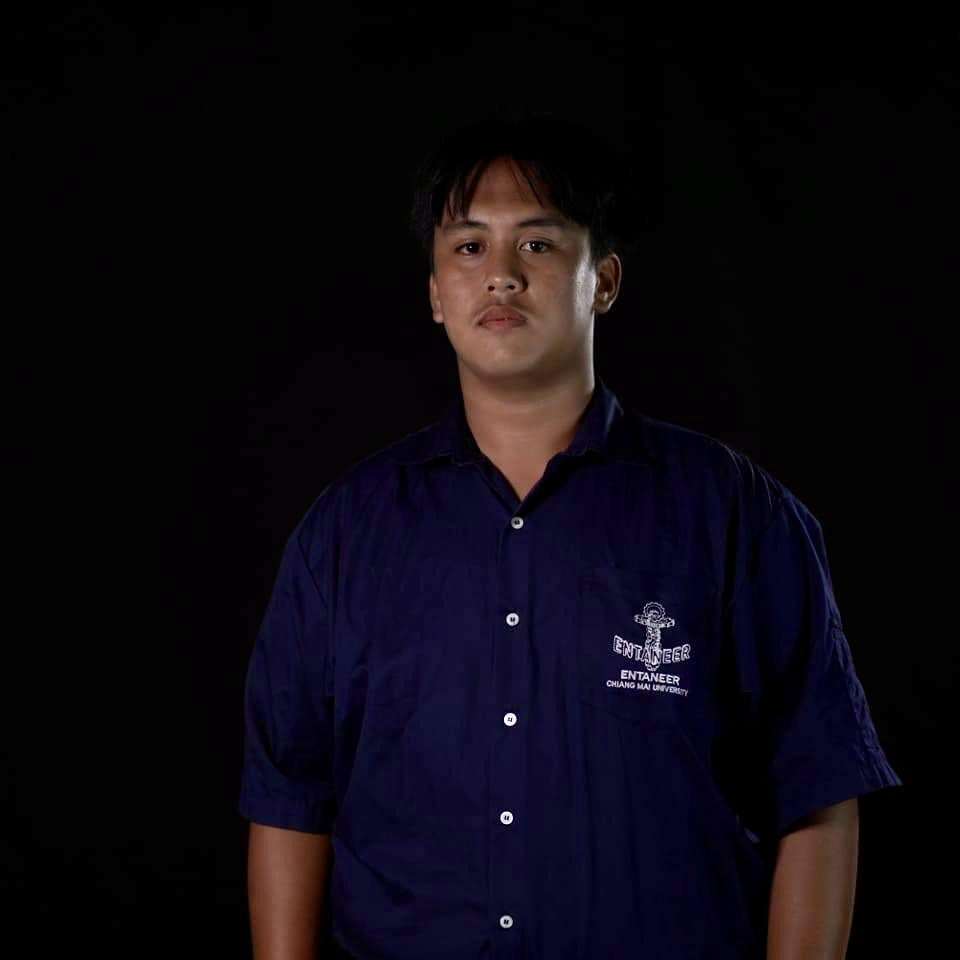
\includegraphics[width=2in]{images/mai_profile.JPEG}
\end{center}
ชื่อ-สกุล: นายปุณณวิชญ์ เดชอินทร์ \\
รหัสนักศึกษา: 650610787 \\
การศึกษา: ปริญญาตรี สาขาวิศวกรรมคอมพิวเตอร์ คณะวิศวกรรมศาสตร์ มหาวิทยาลัยเชียงใหม่ \\
Email: punnawich\_dachin@cmu.ac.th
\end{biosketch}

\begin{biosketch}
\begin{center}
  
\includegraphics[width=1.5in]{peet.png}
\end{center}
ชื่อ-สกุล: นายรัชพล แปรงทอง \\
รหัสนักศึกษา: 650610802 \\
การศึกษา: ปริญญาตรี สาขาวิศวกรรมคอมพิวเตอร์ คณะวิศวกรรมศาสตร์ มหาวิทยาลัยเชียงใหม่ \\
Email: ratchapon\_pra@cmu.ac.th
\end{biosketch}

% the \texttt{biosketch} environment.
% \end{biosketch}


\fi % \ifproject
\end{document}
